\documentclass{scrreprt}
\usepackage{amssymb}
\usepackage{mathtools}
\usepackage{dsfont}
\usepackage{scrhack}
\usepackage{graphicx}
\usepackage{caption}
\usepackage{subcaption}
\usepackage{pgfplots}
\usepackage{listings}
\usepackage{xcolor}
\usepackage{framed}
\usepackage{url}

\lstset { %
    language=C++,
    backgroundcolor=\color{black!5}, % set backgroundcolor
    basicstyle=\footnotesize,% basic font setting
}

\pgfplotsset{compat=1.12}
\pgfplotsset{soldot/.style={color=blue,only marks,mark=*}}
\pgfplotsset{holdot/.style={color=blue,fill=white,only marks,mark=*}}

% Set counter for section
\setcounter{section}{1}
\setcounter{subsection}{1}
\setcounter{tocdepth}{1}

% new commands
\newcommand{\qed}{$\hfill\blacksquare$}
% new commands (end)

% new theorems
\newtheorem{theorem}{Theorem}[chapter]
\newtheorem{lemma}[theorem]{Lemma}
\newtheorem{proposition}[theorem]{Proposition}
\newtheorem{corollary}[theorem]{Corollary}
\newtheorem{definition}[theorem]{Definition}
\newtheorem{example}[theorem]{Example}
\newtheorem{remark}[theorem]{Remark}
\newtheorem{algorithm}[theorem]{Algorithm}
% new theorems (end)

% new environments
\newenvironment{proof}[1][Proof]{\begin{trivlist}
\item[\hskip \labelsep {\bfseries #1}]}{\end{trivlist}}
\newenvironment{describe}[1][]{\begin{trivlist}
\item[\hskip \labelsep {\bfseries #1}]\itshape}{\end{trivlist}}
% new environments (end)

\begin{document}

\pagenumbering{Roman} % set page numbering to Roman

% title_page
\begin{titlepage} % (fold)

    \begin{center}
        \begin{Large}
            Universit\"at Regensburg\\
            Fakult\"at f\"ur Mathematik\\
        \end{Large}
        \vspace{0.5cm}
        \begin{huge}
            \textbf{Solving Convex and Non-Convex Functionals in Image Processing using a Primal-Dual Algorithm}
        \end{huge}
        \vspace{0.5cm}
        \begin{center}
        
\includegraphics[width=8cm]{img/sigillum.png}
        \vspace{0.5cm}\\
        \begin{Large}
            \textbf{MASTERARBEIT}\\
        \end{Large}
        \vspace{0.5cm}
        \begin{large}
            zur Erlangung des akademischen Grades\\
            Master of Science\\
            im Studiengang Computational Science\\
            \vspace{0.5cm}
            Eingereicht bei Prof. Dr. Harald Garcke\\
            am 28.02.2016
        \end{large}
        \vspace{0.5cm}
    \end{center}

    \begin{flushleft}
        \begin{large}
            Vorgelegt von:\\
            Michael Bauer\\
            Banater Str. 1\\
            84061 Ergolsbach\\
            Geboren am 23.08.1987 in Gr\"afelfing
            % Matrikelnummer: 152 8558
        \end{large}
    \end{flushleft}

    \end{center}

\end{titlepage}
% title_page (end)

\newpage

\chapter*{Abstract} % (fold)
\label{cha:abstract}

    Studying three different functionals in image processing, namely ROF, TVL1 and Mumford-Shah, lead to a variety of interesting applications. These models are based on minimization problems and can efficiently be solved by using a primal-dual algorithm. Whereas minimizing the ROF and TVL1 functionals are convex optimization problems, minimization of the Mumford-Shah functional is a non-convex problem. In order to overcome the non-convexity, convex relaxation techniques are used. This leads to a convex saddle-point formulation of the problem and can therefore also be solved using the primal-dual algorithm. However, the algorithm itself converges slowly to the optimal solution in the case of the Mumford-Shah functional. This is related to Dykstra's projection algorithm, which is used in each iteration step of the primal-dual algorithm. To resolve the run-time issue, we present a method for solving the convex relaxed Mumford-Shah model using Lagrange Multipliers. It creates at least a factor 450 run-time performance increase compared to the version based on Dykstra projections. Further, we consider an approach to the Mumford-Shah functional, which is able to compute the minimizer of this functional in real-time. With these three models we present a variety of applications to imaging, like image approximation, cartooning, denoising and inpainting.
    
% chapter abstract (end)

\newpage

\chapter*{Acknowledgements} % (fold)
\label{cha:acknowledgements}
	
    The last step to obtain the title Master of Science in Computational Science, was this thesis. I could never have done it without the support of several people. Now, I get the chance to thank everybody who contributed directly or indirectly and gave me assistance, whenever I needed it.
    
    For being patient, supportive, motivating and always positive I have to thank you so much Sylvia. For your patience also lot of thanks to my mother. For fruitful discussions, listening to all my talks at least once and correcting silly sentences I want to thank Leonie and Bernhard. For the great discussions about programming thank you Michael.
    
    The basis of this thesis are the works published by Prof. Dr. Daniel Cremers (TUM). Thanks to you and your group, especially Thomas Moellenhoff, for the chance to join the CUDA course and for your external contribution to this work.
    
    The thesis itself was written at the chair of Prof. Dr. Harald Garcke, who also supervised me. Thank you so much for your support, input and the freedom you gave in this work.

% chapter acknowledgements (end)

\newpage

% Content, Tables, Figures
\tableofcontents
\listoftables
\listoffigures
% Content, Tables, Figures (end)

\pagenumbering{arabic} % set page numbering back to arabic

\chapter{Introduction} % (fold)
\label{cha:introduction}

    In the second decade of the twenty-first century autonomous driving seems to be the big thing for the car, computer and software industry. The expectation is nothing less than having fewer, or even no, accidents. With these cars, industry is trying to change the world to a better. As this may comfort many people, it poses a lot of computational issues, for instance a stable hardware or even more important viable software. One field of research - of many others - is called Machine Learning, where the computer is trained to make the right decisions in the right situations. The car should be able to accommodate to all possible circumstances which could appear during a drive. To make it even more complicated, the car needs to decide in real-time. As one can imagine, it is extremely difficult to develop fast, stable and tractable methods.\\
    To learn from a certain situation, the car and the computer, respectively, need data from the environment. This can be the shape of another car, traffic lights, differences in the lighting conditions or the distance to other objects. What all these information have in common: they can be collected via images. Small cameras are tracking the traffic and surrounding and for this providing necessary data.\\
    But it is not only the autonomously driving car which make use of images. Doctors use X-ray view or MRI scans in patient treatment, semiconductor companies use pictures of wafers seeking for damages on it, for example scratches or dark spots and unfortunately, images are also used in modern warfare. For this reason, image processing has become more important during the last decades. Researchers dealt with many problems like edge detection, deblurring, denoising, inpainting or image segmentation. In the field of edge detection the probably most famous researcher is John F. Canny. He provided the first tractable and stable edge detection algorithm, presented in 1986 (c.f. \cite{Canny}).\\
    Only three years after Canny published his work, two researchers, namely David Mumford and Jayant Shah, published a paper (\cite{Mumford-et-al-cpam}), whose impact is still present. To date their publication of the so called Mumford-Shah functional was cited over 4.664 times (as of February 14th 2016). They proposed to minimize the energy of the functional in order to approximate an input image optimally. Solving this optimization problem leads to applications like image denoising, inpainting and segmentation. Unfortunately, this functional is by definition non-convex. For this reason finding the minimal energy of it is a hard task.\\
    One approach to compute the minimizer is by using convex relaxation techniques. We can rewrite the non-convex minimization into a convex saddle-point problem. With this reformulation we are able to apply a primal-dual algorithm and therefore solve the optimization problem. Since, this approach leads to a long run-time, we will contribute another version of the proposed saddle-point formulation. It leads to a speed-up by a factor 450. The quickest method for minimizing the Mumford-Shah functional is probably the real-time framework proposed by Strekalovskiy and Cremers in 2014. This approach is more in the sense of modern technology and applicable for image cartooning and denoising, as well as unsupervised segmentation.\\
    Another approach to image processing was proposed in 1992. The researchers Rudin, Osher and Fatemi focused on total variation based imaging. They stated a convex minimization problem, namely the ROF model. Applications, which arise from these models, are for instance, removing Gaussian noise from a given input image or image inpainting. Even, if this model is not as accurate as the Mumford-Shah model, we will show, that it is much easier to solve and tractable for real-time computations.\\
    In the ROF model we find a data term based on the $L^{2}$ norm. By replacing this norm with the $L^{1}$ norm, we derive the so called TVL1 model, hence the name. It is again a convex model and the energy of the functional can therefore easily be minimized. We will show, that this is by far the best model to remove salt and pepper noise from input images. It is also accurate in removing Gaussian noise.\\
    In this work, we present all of these models, compare them against each other and estimate applicable parameters used in the models itself. We further present the primal-dual algorithm, which is the framework to solve all minimization problems. Since, this algorithm is a solver for saddle-point problems, we also clarify how we turn a minimization into a saddle-point problem. All this is summarized in a computer program with the name \textit{iPAUR}, which is available online. The desired hope is, that the applications of these models are used to solve the new challenges arising in industry or medicine.
    
% chapter introduction (end)

\chapter{Basic Concepts} % (fold)
\label{cha:basic_concepts}

    In this chapter we give an introduction to the most important concepts we meet in this thesis. We start by defining images in a mathematical manner, then introduce basic concepts of convex analysis and the total variation.
    \section{Images in Mathematics} % (fold)
    \label{sec:images_in_mathematics}

        Images can be viewed as mathematical objects. We can distinguish between discrete and continuous images. Let us first introduce images in the mathematical sense and then give some examples. The definition and examples can be found in \cite{Bredies}, in german.

        \begin{definition}[Image] % (fold)
        \label{def:image}

            Let $\Omega \subseteq \mathbb{R}^{n}$ be an image domain and $C$ be a color space. A n-dimensional image $u$ is a mapping $u: \Omega \longrightarrow C$, where each point in $\Omega$ corresponds to a color value in $C$.

        \end{definition}
        % definition image (end)

        \begin{remark}[Continuous and discrete images] % (fold)
        \label{rem:continuous_vs_discrete}
            
            Images can be discrete or continuous. The difference between these two classes is determined in the image domain $\Omega$.
                \begin{itemize}
                    \item Let $\Omega = \{ 1, ..., N \}^{n}$, then $u$ is a discrete image, since $\Omega$ is a discrete set. All images on our computers are discrete, because each singel pixel lies at a fixed, discrete position $(i,j)$.
                    \item Let $\Omega \subseteq \mathbb{R}^{n}$, then $u$ is a continuous image. For instance, we could set $\Omega = [a, b]^{n}$ with $a, b \in \mathbb{R}$ and $a < b$.
                \end{itemize}
            There are several image types like binary images, or colored images. The property, to which type an image $u$ belongs, is determined by the color space $C$:
                \begin{itemize}
                    \item Let $C = \{ 0, 1 \}$, then we call $u$ binary.
                    \item In the case of grayscaled images we set $C = \{ 0, ..., 2^{k}-1 \}$, where the value $k$ determines the bit depth. Usually, we find in computers $k = 8$, i.e. grayscaled images take on values in between $0$ and $255$, where $0 = \textnormal{black}$ and $255 = \textnormal{white}$.
                    \item A n-dimensional color image has $C = \{ 0, ..., 2^{k}-1 \}^{n}$, where - for instance - $n = 3$.
                    \item As a last example an image $u$ could also map to continuous color spaces, e.g. 

                    $C = [a, b]^{n}$ or $C = \mathbb{R}^{n}$. Most common are RGB (red-green-blue) images with $n = 3$, $a = 0$ and $b = 1$.
                \end{itemize}

            In this thesis we consider two cases for the domain $\Omega$. One where $\Omega$ is two-dimensional, and the other where $\Omega$ is a three-dimensional space. In the first case, we call a point $(i, j)$ in $\Omega$ pixel, in the second case a point $(i, j, k)$ is called voxel.

        \end{remark}
        % remark continuous_vs_discrete (end)

        \begin{figure}[!ht]
            \centering
                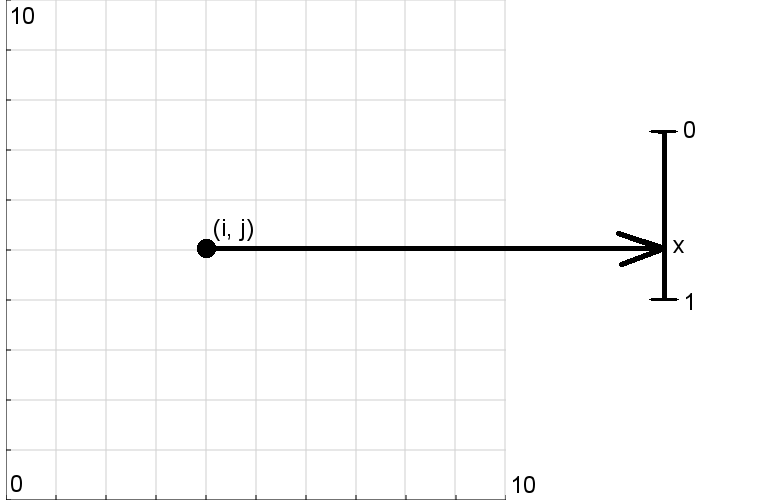
\includegraphics[width=0.6\textwidth]{img/image_mapping.png}
            \caption[Mapping of images.]{A function $u: \{0,1,...,10\}^{2} \to [0,1]$, mapping a pixel $(i,j)$ to the value $x \in [0,1]$.}
        \label{fig:image_mapping}
        \end{figure}

        In the following we use the notation $\mathbb{R}_{\infty}$ for the extended real-values, namely $\mathbb{R} \cup \{ \infty \}$, and $\mathbb{R}_{+}$ is used equivalently to $\mathbb{R}_{> 0}$.

    % section images_in_mathematics (end)

    \section{Convex Optimization and Convex Analysis} % (fold)
    \label{sec:convex_optimization_and_convex_analysis}

        In this section we cover a few topics which are related to convex analysis. Since we are facing convex optimization problems, we first define a convex program, where we mainly follow the book Convex Optimization by Stephen Boyd (\cite{Boyd}).

        An optimization problem is of the form
            \begin{equation}
                \begin{array}{l l l}
                    \min\limits_{u \in \mathbb{R}^{n}} & F(u) & \\
                    \textnormal{subject to} & G_{i}(u) \le 0, & i = 1, ..., m \\
                    & H_{j}(u) = 0 & j = 1, ..., p,
                \end{array}
                \label{eq:optimization_problem_original}
            \end{equation}
        where
            \begin{itemize}
                \item $u \in \mathbb{R}^{n}$ is called the optimization variable,
                \item $F: \mathbb{R}^{n} \longrightarrow \mathbb{R}$ objective function or cost function,
                \item $G_{i}(u) \le 0$ inequality constraints for all $i = 1, ..., m$,
                \item $H_{j}(u) = 0$ equality constraints for all $j = 1, ..., p$,
                \item $G_{i}: \mathbb{R}^{n} \longrightarrow \mathbb{R}$ for all $i = 1, ..., m$ the inequality constraint functions and
                \item $H_{j}(u) = 0$ for all $j = 1, ..., p$ the equality constraint functions.
            \end{itemize}
        If we have no constraints, meaning $m = p = 0$, we call the system \ref{eq:optimization_problem_original} unconstrained. It is a convex optimization problem if all, the objectiv, equality and inequality functions, are convex. We call a point $u$ feasible if it satisfies all constraints. The optimization problem \ref{eq:optimization_problem_original} is said to be feasible if there exists at least one feasible point, and infeasible otherwise. We define the optimal value $u^{\ast}$ of the system \ref{eq:optimization_problem_original} by
            $$
                u^{\ast} = \inf \left\{ F(u) : G_{i}(u) \le 0, \,\, i = 1, ..., m, \,\, H_{j}(u) = 0, \,\, j = 1, ..., p \right\},
            $$
        where we allow $u^{\ast}$ to take on the extended values $\pm \infty$. We set $u^{\ast} = \infty$ if the problem is infeasible, since $\inf(\emptyset) = \infty$. If there are feasible points $u_{k}$ with $F(u_{k}) \to -\infty$ as $k \to \infty$, then $u^{\ast} = -\infty$, and we say that problem \ref{eq:optimization_problem_original} is unbounded below.

        Since, convex optimization is based on convex analysis we define the class of convex functions and its properties. We set $X \subseteq \mathbb{R}^{n}$ and its dual space $Y = X^{\ast}$. Relating to Chambolle et al. in \cite{Chambolle-et-al-10}, we have the following basic definitions, propositions and theorems.

        \begin{definition}[Convex Set] % (fold)
        \label{def:convex_set}

            A subset $C \subseteq \mathbb{R}^{n}$ is said to be convex if and only if for any $u_{1}, u_{2} \in C$, the line segment $[u_{1}, u_{2}] \subseteq C$, that is, for any $t \in [0, 1]$,
                $$
                    u_{1}t + u_{2}(1 - t) \in C.
                $$
        \end{definition}
        % definition convex_set (end)

        This definition ensures that if $C$ is convex, we can always find two arbitrary points in $C$, such that the line segment $[u_{1}, u_{2}]$ with end points $u_{1}, u_{2}$ lies fully in $C$ (see figure \ref{fig:convex_and_non_convex_sets}).
        \begin{figure}[!ht]
            \centering
            \begin{subfigure}[b]{0.3\textwidth}
                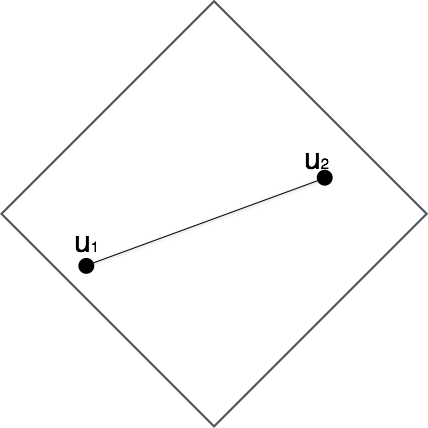
\includegraphics[width=\textwidth]{img/unit_l1_norm.png}
                \caption{$l_{1}$ unit sphere}
            \end{subfigure}
            \begin{subfigure}[b]{0.3\textwidth}
                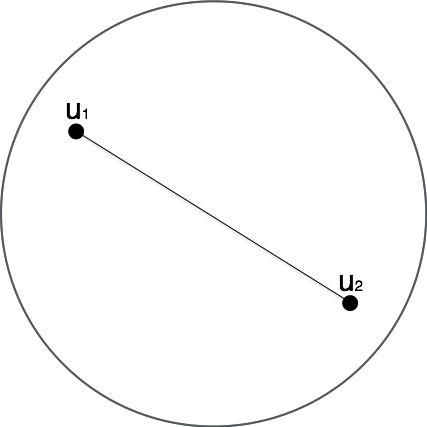
\includegraphics[width=\textwidth]{img/unit_l2_norm.png}
                \caption{$l_{2}$ unit sphere}
            \end{subfigure}
            \begin{subfigure}[b]{0.3\textwidth}
                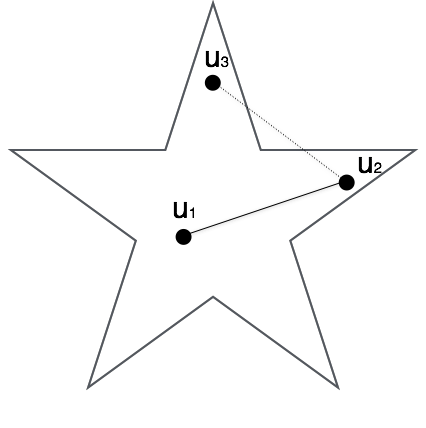
\includegraphics[width=\textwidth]{img/non_convex_set.png}
                \caption{Star: a non-convex set.}
            \end{subfigure}
            \caption[Examples of convex sets.]{Three different sets, where (a) and (b) are convex, but (c) is not. (a) refers to the unit sphere of the $l^{1}$ norm, where (b) refers to the unit sphere of the $l^{2}$ norm. In (c) we see that the line segment of $[u_{2}, u_{3}]$ lies not in the set itself.}
            \label{fig:convex_and_non_convex_sets}
        \end{figure}

        \begin{definition}[Indicator Function, Support Function] % (fold)
        \label{def:indicator_function}

            For any subset $C \subseteq X$ of a vector space, the indicator function $\delta_{C}: X \longrightarrow \mathbb{R}_{\infty}$ is defined as
                $$
                    \delta_{C}(u) =
                    \left\{
                        \begin{array}{l l}
                          0      & \quad \text{if $u \in C$}, \\
                          \infty & \quad \text{if $u \notin C$}.
                        \end{array}
                    \right.
                $$
            The support function of the set $C$ is defined as
                $$
                    S_{C}(u) = \sup_{p \in C} \langle p, u \rangle,
                $$
            where we allow $S_{C}(u)$ to be $+\infty$.
     
        \end{definition}
        % definition indicator_function (end)

        \begin{definition}[Convex Function, Proper, Lower-Semicontinuous] % (fold)
        \label{def:convex_function_proper_lower_semicontinuous}

            Let $C \subseteq \mathbb{R}^{n}$ be a convex set. A function $F: C \longrightarrow \mathbb{R}_{\infty}$ is said to be
                \begin{itemize}
                    \item convex if and only if for all $u_{1}, u_{2} \in C$ and any $t \in [0, 1]$ the inequality
                    \begin{equation}
                        F(u_{1}t + u_{2}(1 - t)) \le F(u_{1})t + F(u_{2})(1 - t)
                        \label{eq:convex_function}
                    \end{equation}
                    is satisfied. $F$ is called strictly convex, if the inequality \ref{eq:convex_function} holds strictly, whenever $u_{1}, u_{2}$ are distinct points and $t \in (0, 1)$.
                    \item proper if and only if $F$ is not identically $-\infty$ or $+\infty$.
                    \item lower-semicontinuous (l.s.c) if and only if for any $u \in C$ and a sequence $(u_{n})$ converging to $u$,
                        $$
                            F(u) \le \liminf_{n \rightarrow \infty} F(u_{n}).
                        $$
                \end{itemize}
            We define $\Gamma_{0}(C)$ as the set of all convex, proper, l.s.c. functions on $C$.

        \end{definition}
        % definition convex_function_proper_lower_semicontinuous (end)

        A common example for a strictly convex function would be a quadratic function, c.f. example \ref{ex:convex_function} and figure \ref{fig:convex_function} (a). It is illustrated, together with the plot in (b) of the function
            \begin{equation}
                F(u) =
                    \begin{dcases*}
                        u^{2} & \textnormal{$x \in [-1, 1]$} \\
                        - \frac{1}{2} u(u - 4) & \textnormal{$x \in (1, 3]$},
                    \end{dcases*}
                \label{eq:lsc_example}
            \end{equation}
        being lower-semicontinuous.

        \begin{proposition} % (fold)
            Let $F, G: X \longrightarrow \mathbb{R}_{\infty}$ be two convex functions. Then $F + G$ is also convex.
        \end{proposition}
        % proposition (end)

        \begin{proof} % (fold)
            Define $H(u) = F(u) + G(u)$ with $F, G$ convex and choose $u_{1}, u_{2} \in X$ and $t \in [0, 1]$. Then we obtain
            \begin{eqnarray}
                H(u_{1}t + u_{2}(1 - t)) &=& F(u_{1}t + u_{2}(1 - t)) + G(u_{1}t + u_{2}(1 - t)) \notag \\ 
                &\le& F(u_{1})t + F(u_{2})(1 - t) + G(u_{1})t + G(u_{2})(1 - t) \notag \\
                &=& \underbrace{F(u_{1})t + G(u_{1})t}_{= H(u_{1})t} + \underbrace{F(u_{2})(1 - t) + G(u_{2})(1 - t)}_{H(u_{2})(1 - t)} \notag \\
                &=& H(u_{1})t + H(u_{2})(1 - t). \notag
            \end{eqnarray}\qed
        \end{proof}
        % proof (end)

        \begin{remark}[Concave Function] % (fold)
            \label{rem:concave_function}

            If $-F$ is (strictly) convex, then we say that $F$ is (strictly) concave. If $F$ is both convex and concave we say that $F$ is affine, i.e. equality holds in equation \ref{eq:convex_function}.

        \end{remark}
        % remark concave_function (end)

        \begin{figure}[!ht]
            \centering
            \begin{subfigure}[b]{0.4\textwidth}
            \begin{tikzpicture}[scale=0.8]
                \begin{axis}
                    \addplot[domain=-3:3,blue] {x*x};
                    \addplot[domain=-1:2,black] {x + 2};
                \end{axis}
            \end{tikzpicture}
            \caption{A quadratic function.}
            \end{subfigure}
            \begin{subfigure}[b]{0.4\textwidth}
            \begin{tikzpicture}[scale=0.8]
                \begin{axis}
                    \addplot[domain=-1:1,blue] {x*x};
                    \addplot[domain=1:3,blue] {-0.5*x*(x-4)};
                    \draw[dotted] (axis cs:1,-1) -- (axis cs:1,3);
                    \addplot[soldot] coordinates{(1,1)};
                    \addplot[holdot] coordinates{(1,1.5)};
                \end{axis}
            \end{tikzpicture}
            \caption{A l.s.c. function.}
            \end{subfigure}
            \caption[Example of convex and l.s.c. function.]{(a) The plot of one line segment above a quadratic function, which lies completely in $\textnormal{epi}(F)$. (b) The lower term $u^{2}$ accesses the value $(1,1)$, but the upper term of the function $-\frac{1}{2}u(u-4)$ does not.}
            \label{fig:convex_function}
        \end{figure}

        \begin{example} % (fold)
        \label{ex:convex_function}

            \begin{enumerate}
                \item Let $A \in \mathbb{R}^{m \times n}$ be a real matrix and $F: \mathbb{R}^{n} \longrightarrow \mathbb{R}^{m}$ a linear function with $F(u) = Au$. Then $F$ is convex and concave, hence linear functions are affine.
                    \begin{proof} % (fold)
                        Choose $u_{1}, u_{2} \in \mathbb{R}, t \in [0, 1]$. We get
                        $$
                           F(u_{1}t + u_{2}(1 - t)) = F(u_{1}t) + F(u_{2}(1 - t)) = F(u_{1})t + F(u_{2})(1 - t)
                        $$
                        by definition of linearity.\qed
                    \end{proof}
                    % proof (end)
                \item Let $A \in \mathbb{R}^{n \times n}$ be a real, symmetric, positiv definite matrix and $F: \mathbb{R}^{n} \longrightarrow \mathbb{R}^{n}$ a linear function with $F(u) = \frac{1}{2}u^{T}Au + b^{T}u = \frac{1}{2}||u||_{A}^{2} + b^{T}u$, where $||\cdot||_{A}^{2}$ denotes the quadratic $A$ (matrix) norm. Then $F$ is strictly convex. We can verify this with $t \in (0, 1)$ and
                    \begin{eqnarray}
                        F(u_{1}t + u_{2}(1-t)) &=& \frac{1}{2} ||u_{1}t + u_{2}(1-t)||_{A}^{2} + b^{T}(u_{1}t + u_{2}(1-t)) \notag \\
                        &\overbrace{\le}^{(\ast)}& \frac{1}{2} \left(||u_{1}t||_{A}^{2} + ||u_{2}(1-t)||_{A}^{2}\right) + (b^{T}u_{1})t + (b^{T}u_{2})(1-t) \notag \\
                        &=& \frac{1}{2} \left( \underbrace{t^{2}||u_{1}||_{A}^{2}}_{< t||u_{1}||_{A}^{2}} + \underbrace{(1-t)^{2}||u_{2}||_{A}^{2}}_{< (1-t)||u_{2}||_{A}^{2}} \right) + (b^{T}u_{1})t + (b^{T}u_{2})(1-t) \notag \\
                        &<& \underbrace{\frac{1}{2} t||u_{1}||_{A}^{2} + (b^{T}u_{1})t}_{= F(u_{1})t} + \underbrace{\frac{1}{2} (1-t)||u_{2}||_{A}^{2} + (b^{T}u_{2})(1-t)}_{= F(u_{2})(1-t)} \notag \\
                        &=& F(u_{1})t + F(u_{2})(1-t). \notag
                    \end{eqnarray}
                In $(\ast)$ we used the triangle inequality.
                \item Each norm $||\cdot||: X \longrightarrow \mathbb{R}$ on a normed vector space $X$ is convex (see also figure \ref{def:convex_function_proper_lower_semicontinuous} for the $l_{1}$ and $l_{2}$ norm).
                    \begin{proof} % (fold)
                        Choose $u, v \in X, t \in [0, 1]$, then
                        $$
                            ||ut + v(1 - t)|| \overbrace{\le}^{(\ast)} ||ut|| + ||v(1 - t)|| \overbrace{=}^{(\ast\ast)} ||u|| t + ||v|| (1 - t).
                        $$
                        In $(\ast)$ we used the triangle inequality and in $(\ast\ast)$ absolute homogeneity with the fact that $t \in [0, 1]$ and for that $(1-t) \in [0,1]$.\qed
                    \end{proof}
                    % proof (end)
            \end{enumerate}

        \end{example}
        % example convex_function (end)

        Another definition of convex functions can sometimes be found in literature, for instance in \cite{Rockafellar}. Therefore, let us first introduce the epigraph and the domain of a function.

        \begin{definition}[Domain, Epigraph] % (fold)
        \label{def:domain_epigraph}

            For any function $F: X \longrightarrow \mathbb{R}_{\infty}$, we define the domain
                $$
                    \textnormal{dom}(F) = \{ u \in X : F(u) < +\infty \},
                $$
            and the epigraph
                $$
                    \textnormal{epi}(F) = \{ (u, t) \in X \times \mathbb{R}: t \ge F(u) \} \in \mathbb{R}^{n+1}.
                $$
        \end{definition}
        % definition domain_epigraph (end)

        Then we have the following definition for convex functions.

        \begin{definition}[Convex Function] % (fold)
        \label{def:convex_function_else}

            A function $F: X \longrightarrow \mathbb{R}_{\infty}$ is convex if $\textnormal{dom}(F)$ and $\textnormal{epi}(F)$ are convex sets.

        \end{definition}
        % definition convex_function_else (end)

        \begin{definition}[Closed Function] % (fold)
        \label{def:closed_function}

            Let $F: X \longrightarrow \mathbb{R}_{\infty}$ be a convex function. Then $F$ is closed if $\textnormal{epi}(F)$ is a closed set.

        \end{definition}
        % definition closed_function (end)

        \begin{figure}[!ht]
            \centering
            \begin{tikzpicture}
                \begin{axis}
                    \addplot[domain=-1:1,black,fill=gray] {0.5*x*x};
                    \draw[red] (axis cs:-1,0) -- (axis cs:1,0);
                    \draw[red] (axis cs:-1,-0.02) -- (axis cs:-1,0.02);
                    \draw[red] (axis cs:1,-0.02) -- (axis cs:1,0.02);
                \end{axis}
            \end{tikzpicture}
            \label{fig:domain_epigraph}
            \caption[Domain and Epigraph.]{The domain (red) denoted as $\textnormal{dom}(F) = [-1, 1]$ and epigraph \\$\textnormal{epi}(F) = \{(u, t) \in [-1, 1] \times \mathbb{R} : t \ge \frac{1}{2}u^{2}\}$ (gray) of a function $F: [-1, 1] \longrightarrow \mathbb{R}$ with $F(u) = \frac{1}{2}u^{2}$.}
        \end{figure}

        Now, that we are set up with convexity, we want to introduce an important concept, which is used in this thesis.

        \begin{definition}[Legendre-Fenchel conjugate] % (fold)
        \label{def:legendre_fenchel_conjugate}

            Let $F: X \longrightarrow \mathbb{R}_{\infty}$ be a convex function. We define the Legendre-Fenchel conjugate $F^{\ast}$ of $F$ for any $p \in Y$ by
                \begin{equation}
                    F^{\ast}(p) = \sup_{u \in X} \left( \langle p, u \rangle - F(u) \right).
                    \label{eq:legendre_fenchel_conjugate}
                \end{equation}

        \end{definition}
        % definition legendre_fenchel_conjugate (end)

        \begin{remark} % (fold)
            \begin{itemize}
                \item Without a proof we state that $F^{\ast}$ - as the supremum of linear, continuous functions - is convex and lower-semicontinous, even $F$ is not convex. In addition, $F^{\ast}$ is proper if $F$ is convex and proper.
                \item In some literature the Legendre-Fenchel conjugate is also denoted as convex conjugate. We use these two expressions equivalently.
            \end{itemize}
        \end{remark}
        % remark (end)

        \begin{theorem} % (fold)
            Let $F \in \Gamma_{0}(X)$, then $F^{\ast\ast} = F$.
        \end{theorem}
        % theorem (end)

        The last theorem assures that we can rewrite equation \ref{eq:legendre_fenchel_conjugate} into
            $$
                F(u) = \left( F^{\ast}(p) \right)^{\ast}(u) = \sup_{p \in X^{\ast}} \left( \langle u, p \rangle - F^{\ast}(p) \right).
            $$
        A proof of this theorem can be found in \cite{Rockafellar}.
        \begin{example}
        \label{ex:legendre_fenchel_conjugate_example}

            Let us view some examples on the Legendre-Fenchel conjugate.
            \begin{enumerate}
                \item The Legendre-Fenchel conjugate of the indicator function of a set $C \subseteq X$ is given by
                    $$
                        \delta^{\ast}_{C}(p) = \sup_{u \in X} \left( \langle p, u \rangle - \delta_{C}(u) \right) = \sup_{u \in C} \langle p, u \rangle,
                    $$
                which is the support function of the set $C$.
                \item Let $F: X \to \mathbb{R}_{\infty}$ be a convex function and $\alpha > 0$. Then the convex conjugate of $\alpha F(u)$ is given by
                    $$
                        \alpha F^{\ast}(\frac{p}{\alpha}).
                    $$
                To verify this equality, we compute
                    $$
                        F^{\ast}(p) = \sup_{u \in X} \left( \langle p, u \rangle - \alpha F(u) \right) = \alpha \underbrace{\sup_{u \in X} \left( \langle \frac{p}{\alpha}, u \rangle - F(u) \right)}_{= F^{\ast}(\frac{p}{\alpha})} = \alpha F^{\ast}(\frac{p}{\alpha}),
                    $$
                which shows the desired equation.
                \item Now, let $||\cdot||$ be a norm on $X$, with dual norm $||\cdot||_{\ast}$ on $Y$. We show that
                    $$
                        F^{\ast}(p) =
                            \begin{dcases*}
                                0 & \textnormal{if $||p||_{\ast} \le 1$,} \\
                                \infty & \textnormal{else},
                            \end{dcases*}
                        = \delta_{||p||_{\ast} \le 1}(p),
                    $$
                i.e. the convex conjugate of a norm is the indicator function of the unit ball of its dual norm.

                \begin{proof}
                    We have
                        $$
                            F^{\ast}(p) = \sup_{u \in X} \left( \langle p, u \rangle - ||u|| \right).
                        $$
                    First assume that $||p||_{\ast} > 1$. By definition of the dual norm ($||p||_{\ast} = \sup\limits_{||x|| \le 1} |\langle p, x \rangle|$) there is a $x \in \mathbb{R}^{n}$ for which we observe that $\langle p, x \rangle > 1$. We set $u = tx$ and let $t \longrightarrow \infty$, then we have
                        $$
                            \langle p, u \rangle - ||u|| = t(\langle p, x \rangle - ||x||) \longrightarrow \infty.
                        $$
                    This shows $F^{\ast}(p) = \infty$. On the other hand if we assume that $||p||_{\ast} \le 1$, Cauchy-Schwarz-inequality assures
                        $$
                            \langle p, u \rangle \le ||u|| \, ||p||_{\ast},
                        $$
                    for all $u \in X$. But this implies
                        $$
                            \langle p, u \rangle - ||u|| \le ||u|| \, ||p||_{\ast} - ||u|| = ||u|| \, (||p||_{\ast} - 1) \le 0.
                        $$
                    Since $||p||_{\ast} \le 1$ holds, we need to choose $u = 0$ to attain the supremum in $F^{\ast}(p)$. This shows that $F^{\ast} = \sup\limits_{u \in X} \left( \langle p, 0 \rangle - ||0|| \right) = 0$.\qed
                \end{proof}
                \item As a last example we show that for a function $F(u) = \frac{1}{2} ||u||^{2}$ its convex conjugate is $F^{\ast}(p) = \frac{1}{2} ||p||_{\ast}^{2}$. With Cauchy-Schwarz-inequality we have $\langle p, u \rangle \le ||p||_{\ast}\,||u||$. Observing
                    $$
                        \langle p, u \rangle - \frac{||u||^{2}}{2} \le ||p||_{\ast}\,||u|| - \frac{||u||^{2}}{2},
                    $$
                where the righthand side is a quadratic function of $||u||$. Define $H(x) := -\frac{x^{2}}{2} + y\,x$, then the maximal value of $H$ is $x = y$, since $H^{'}(x) = -x + y$ and $H^{'}(x) = 0$ implies $x = y$. Plugging $||u||$ into $H$ we have $||u|| = ||p||_{\ast}$. It follows
                    $$
                        \langle p, u \rangle - \frac{||u||^{2}}{2} \le ||p||_{\ast}||u|| - \frac{||u||^{2}}{2} = ||p||_{\ast} ||p||_{\ast} - \frac{||p||_{\ast}}{2} = \frac{||p||_{\ast}^{2}}{2}.
                    $$
                This shows that $F^{\ast}(p) = \sup\limits_{u \in X} \left( \langle u, p \rangle - \frac{||u||_{2}^{2}}{2} \right) \le \frac{||p||_{\ast}^{2}}{2}$. Let us now proof the inequality in the other direction. We assume that we find an arbitrary $u$ which satisfies $\langle u, p \rangle = ||u||\,||p||_{\ast}$. Further, we assume that $||u|| = ||p||_{\ast}$. Then we have
                    $$
                        \langle p, u \rangle - \frac{||u||^{2}}{2} = ||u||\,||p||_{\ast} - \frac{||u||^{2}}{2} = \frac{||p||^{2}_{\ast}}{2},
                    $$
                and conclude
                    $$
                        \frac{||p|_{\ast}^{2}}{2} = \langle p, u \rangle - \frac{||u||^{2}}{2} \le \sup\limits_{u \in X} \left( \langle p, u \rangle - \frac{||u||^{2}}{2} \right) = F^{\ast}(p).
                    $$
                From these two inequalities it follows that $F^{\ast}(p) = \frac{||p||_{\ast}^{2}}{2}$.\qed
            \end{enumerate}
        \end{example}

        Another important property of functions is differentiability. Unfortunately, in some cases a function $F$ is not differentiable everywhere. If such a function is convex, we have a generalization of the derivative, called subdifferential. For this, we want to define the subdifferential and corresponding to it, the subgradient.

        \begin{definition}[Subgradient, Subdifferential] % (fold)
        \label{def:subgradient_subdifferential}

            Let $X \subseteq \mathbb{R}^{n}$ be an open, convex set and $F: X \longrightarrow \mathbb{R}_{\infty}$ a convex function. A vector $y$ is called subgradient of $F$ in $u_{0} \in X$, if
                \begin{equation}
                    F(u) \ge F(u_{0}) + \langle y, u - u_{0} \rangle \,\,\, \forall u \in X.
                \label{eq:subgradient}
                \end{equation}
            The set
                $$
                    \partial F(u_{0}) = \{ y \in X: \, F(u) \ge F(u_{0}) + \langle y, u - u_{0} \rangle \,\,\, \forall u \in \textnormal{dom}(F) \}
                $$
            is called subdifferential of $F$ in $u_{0} \in X$ and $\textnormal{dom}(\partial F) = \{ u: \partial F(u) \ne \emptyset \} \subseteq F$.

        \end{definition}
        % definition subgradient_subdifferential (end)

        If $F$ and $G$ are differentiable, we have $\partial(F + G) = \partial F + \partial G$. For the subdifferential this holds under some conditions. We want to give the corresponding proposition without a proof, for which we refer to \cite{Rockafellar}. But, we state that in our computations this equality can always be used.

        \begin{proposition} % (fold)

            Let $F, G$ be convex and assume $\textnormal{int} (\textnormal{dom} G) \cap \textnormal{dom} F \ne \emptyset$: then
                $$
                    \partial(F + G) = \partial F + \partial G.
                $$
        \end{proposition}
        % proposition (end)

        To illustrate the subgradient and subdifferential, respectively, we want to give some examples.

        \begin{example}
        \label{ex:subgradient_subdifferential}

            \begin{enumerate}
                \item Take the absolute value function $F(u) = |u|$ in $\mathbb{R}$, defined by
                    $$
                        F(u) =
                            \begin{dcases*}
                                u & \textnormal{if $u \ge 0$,} \\
                                -u & \textnormal{else}.
                            \end{dcases*}
                    $$
                Since $F(u)$ is not differentiable in $0$, but on $\mathbb{R} / \{0\}$, we compute the subgradient $y$
                    \begin{itemize}
                        \item $\partial F(u) = 1$ if $u > 0$,
                        \item $\partial F(u) = -1$ if $u < 0$,
                        \item and finally
                            $$
                                F(0) + y (u - 0) \le F(u) \Longleftrightarrow y u \le |u|.
                            $$
                        If $u \ge 0$ this is equivalent to $y \ge 1$. If $u < 0$ we get
                            $$
                                y u \le |u| \Longleftrightarrow y u \le -u \Longleftrightarrow y \ge -1.
                            $$
                    \end{itemize}
                Finally, we summarize
                    $$
                        y =
                            \begin{dcases*}
                                1 & \textnormal{if $u > 0$,} \\
                                -1 & \textnormal{if $u < 0$,} \\
                                [-1, 1] & \textnormal{if $u = 0$.}
                            \end{dcases*}
                    $$
                \item Let $F(u) = ||u||_{1}$ be the convex $l^{1}$ norm, which is defined by
                    $$
                        ||u||_{1} := \sum_{i = 1}^{n} |u_{i}|,
                    $$
                for $u \in \mathbb{R}^{n}$. As a non-differentiable function in $u_{0} = 0$, we seek for the subdifferential. Looking at the i-th component of the subgradient, we evaluate the subgradient of the absolute value function. With example 1., we set $y_{i} = -1$ if $u_{i} < 0$ and $y_{i} = 1$ if $u_{i} > 0$. In the case, where $u_{i} = 0$, we observed $y_{i} \in [-1,1]$. Overall, we set
                    $$
                        y_{i} =
                            \begin{dcases*}
                                1 & \textnormal{if $u_{i} > 0$,} \\
                                -1 & \textnormal{if $u_{i} < 0$,} \\
                                [-1,1] & \textnormal{if $u_{i} = 0$,}
                            \end{dcases*}
                    $$
                for all $i = 1, ..., n$. Note, that for the whole vector $y$ the inequality $||y||_{\infty} \le 1$ is satisfied. Then, the subdifferential is given by
                    $$
                        \partial F(u) = \left\{ y : ||y||_{\infty} \le 1, \, \langle y, u \rangle = ||x||_{1} \right\}.
                    $$
            \end{enumerate}
        \end{example}

        The following proposition can be found in the work of Pock and Chambolle (\cite{Chambolle-et-al-10}). We provide it without a proof.

        % \begin{proposition} % (fold)
        % \label{prop:convex_subgradient}

        %     For any $F$ convex, $p \in \partial F(u)$ if and only if
        %         $$
        %             \langle p, u \rangle - F(u) = F^{\ast}(p).
        %         $$
        %     Moreover, if $F \in \Gamma_{0}$, so that $F^{\ast\ast} = F$, then this is equivalent to $u \in \partial F^{\ast}(p)$.

        % \end{proposition}
        % % proposition convex_subgradient (end)

        \begin{proposition} % (fold)
        \label{prop:zero_element_of_subgradient}
            
            Let $F$ be convex, then $\hat{u} \in \arg \min\limits_{u \in X} F(u)$ if and only if $0 \in \partial F(\hat{u})$.

        \end{proposition}
        % proposition zero_element_of_subgradient (end)

        Another important property of convex minimization problems is summarized in the next proposition. It can be found in \cite{Rockafellar}, along with a proof.

        \begin{proposition} % (fold)
        \label{prop:global_minimum}

            Let $F \in \Gamma_{0}(X)$. Then if $\hat{u}$ is a local minimum of $F$, then $\hat{u}$ is in fact a global minimum, i.e.
                    $$
                        \hat{u} \in \arg \min_{u \in X} F(u).
                    $$
        \end{proposition}
        % proposition (end)

        These propositions give us some important statements. If we find a (local) minimizer of a convex minimization problem, we already know that this minimizer is indeed the global optimum. Further, we can verify that a solution to a minimization problem is valid, if zero is an element of the subdifferential of the cost function at this specific minimal point. With this, we later compute the proximity operator of the functions in our underlying model. This operator is defined in the next definition and is the basis of Moreau' theorem (c.f. theorem \ref{the:moreau_identity}).

        \begin{definition}[Projection Operator, Proximity Operator, Moreau Envelop] % (fold)
        \label{def:projection_operator}

            For any non-empty closed set $C$ the projection operator for an arbitrary point $z \notin C$ on the set $C$ is defined by
                \begin{equation}
                    \Pi_{C}(z) = \arg \min_{u \in C} \frac{1}{2} ||z - u||_{2}^{2},
                \end{equation}
            meaning the orthogonal projection onto the convex set $C$. We define the proximity operator in a similar fashion due to
                \begin{equation}
                    \textnormal{prox}^{\alpha}_{F}(z) = \arg \min_{u \in X} \frac{1}{2} ||u - z||_{2}^{2} + \alpha \, F(u),
                    \label{eq:proximity_operator}
                \end{equation}
            and the Moreau envelop as
                $$
                    M^{\alpha}_{F}(z) = \min_{u \in X} \frac{1}{2} ||u - z||_{2}^{2} + \alpha \, F(u),
                $$
            for any $\alpha > 0$.
        \end{definition}
        % definition projection_operator (end)

        The next theorem, namely Moreau's theorem, was first proven in 1965 by Jean J. Moreau and can be found in \cite{Rockafellar}, along with a proof.

        \begin{theorem}[Moreau's Theorem] % (fold)
        \label{the:moreau_identity}

            Let $F \in \Gamma_{0}(X)$ and $F^{\ast}(p) = \sup\limits_{u \in X} \langle u, p \rangle - F(u)$ be its Legendre-Fenchel conjugate. Then
                $$
                    M^{\alpha}_{F}(z) + M^{\alpha}_{F^{\ast}}(z) = \frac{1}{2}||z||^{2},
                $$
            i.e. for each $z \in \mathbb{R}^{n}$ one has
                $$
                    \min_{u \in X} \left( \frac{1}{2} ||u - z||^{2} +  \alpha \, F(u) \right) + \min_{p \in Y} \left( \frac{1}{2} ||p - z||^{2} +  \alpha \, F^{\ast}(p) \right) = \frac{1}{2}||z||^{2},
                $$
            where both minima are uniquely attained. The unique vectors $u$ and $p$ for which the respective minima are attained for a given $z$ are the unique vectors $u$ and $p$ such that
                \begin{equation}
                    z = u + p, \,\,\,\,\, p \in \partial F(u),
                    \label{eq:equivalence_of_moreau_property}
                \end{equation}
            and they are given by
                \begin{equation}
                    u = \textnormal{prox}^{\alpha}_{F}(z), \,\,\,\,\, p = \textnormal{prox}^{\alpha}_{F^{\ast}}(z).
                    \label{eq:prox_z}
                \end{equation}
        \end{theorem}
        % theorem moreau_identity (end)

        \begin{remark}
            Another way to denote the proximity operator is the notation
                \begin{equation}
                    \textnormal{prox}^{\alpha}_{F} = (\textnormal{Id} + \alpha \partial F)^{-1}.
                    \label{eq:proximity_operator_reloaded}
                \end{equation}
            It can be derived by proposition \ref{prop:zero_element_of_subgradient}. For that, assume that $u \in \textnormal{prox}^{\alpha}_{F}$. Then
                $$
                    0 \in \partial \left( \alpha F(u) + \frac{1}{2} ||u - z||_{2}^{2} \right) = \alpha \, \partial F(u) + u - z.
                $$
            But this can be rewritten as
                $$
                    z \in \alpha\,\partial F(u) + u \Longleftrightarrow u = (\textnormal{Id} + \alpha \, \partial F)^{-1}(z).
                $$
            Furthermore, using equations \ref{eq:equivalence_of_moreau_property}, \ref{eq:prox_z} and \ref{eq:proximity_operator_reloaded}, we get
                \begin{equation}
                    z = (\textnormal{Id} + \alpha \, \partial F)^{-1}(z) + \alpha \left( \textnormal{Id} + \frac{1}{\alpha} \partial F^{\ast} \right)^{-1} \left(\frac{z}{\alpha}\right).
                    \label{eq:moreau_identity_reloaded}
                \end{equation}
            This equation is best known as Moreau's identity.
        \end{remark}

        To this end, let us discuss some examples on the projection and proximity operator, respectively.

        \begin{example}
        \label{ex:projection_operator}

            \begin{itemize}
                \item The $l^{p}$ projection of a point $\tilde{u} \in \mathbb{R}^{n}$ onto the $l^{p}$ unit sphere with $\tilde{u} \notin C = \{u : ||u||_{p} \le 1 \}$ is given by the following minimization problem:
                    \begin{equation}
                        \begin{array}{l l}
                            \min\limits_{u \in C} &  \frac{1}{2} ||u - \tilde{u}||_{2}^{2} \\
                            \textnormal{subject to} & ||u||_{p} \le 1.
                        \end{array}
                        \notag
                    \end{equation}
                According to \cite{Jitkomut} the $l^{2}$ or euclidean projection and the $l^{\infty}$ projection are given by
                    \begin{enumerate}
                        \item $\Pi_{||\cdot||_{2} \le 1}(\tilde{u}) = \frac{\tilde{u}}{\max(1, |\tilde{u}|)}$, or equivalently
                            \begin{equation}
                                u^{\ast} =
                                \left\{
                                    \begin{array}{l l}
                                       \tilde{u}, & \textnormal{if}\,\, ||\tilde{u}||_{2} \le 1 \\
                                       \frac{\tilde{u}}{||\tilde{u}||_{2}}, & \textnormal{otherwise,}
                                    \end{array}
                                \right.
                                \notag
                            \end{equation}
                        \item and $\Pi_{||\cdot||_{\infty} \le 1}(p) = \min(1, \max(-1, p))$, or for all $k = 1, ..., n$
                            \begin{equation}
                                u_{k}^{\ast} =
                                \left\{
                                    \begin{array}{l l}
                                       \tilde{u}_{k}, & \textnormal{if}\,\, |\tilde{u}_{k}| \le 1 \\
                                       1, & \textnormal{otherwise.}
                                    \end{array}
                                \right.
                                \notag
                            \end{equation}
                    \end{enumerate}
                \item If we set $F(u) = \delta_{C}(u)$ then we get
                $$
                    \textnormal{prox}^{\alpha}_{F}(\tilde{u}) = \min\limits_{u \in X} \frac{||u - \tilde{u}||_{2}^{2}}{2} + \alpha \, \delta_{C}(u) = \min\limits_{u \in C} \frac{||u - \tilde{u}||_{2}^{2}}{2} = \Pi_{C}(\tilde{u}).
                $$
                We see a connection between the two operators. Proximation of the indicator function is the same as doing a euclidean projection onto the corresponding set $C$.
            \end{itemize}
        \end{example}

    % section convex_optimization_and_convex_analysis (end)

    \section{Total Variation} % (fold)
    \label{sec:total_variation}
        
        The definition of the total variation, the variation of functions and functions of bounded variation can be found in \cite{Giusti}, together with the first example in this section. The total variation is the basis when talking about variational methods in image processing. We cover this topic superficial, which is enough for the considered classes of problems.

        \begin{definition}[Total Variation] % (fold)
        \label{def:total_variation}

            Let $\Omega$ be an open subset of $\mathbb{R}^{n}$. For a function $u \in L^{1}(\Omega)$, the \textnormal{total variation} of $u$ in $\Omega$ is defined as
                $$
                    \textnormal{TV}(u) = \sup \bigg\{ -\int_{\Omega} u\, \textnormal{div}\, (\varphi)\, dx : \varphi \in C^{1}_{0}(\Omega, \mathbb{R}^{n}), |\varphi(x)| \le 1, \forall x \in \Omega \bigg\}.
                $$
        \end{definition}
        % definition total_variation (end)

        \begin{example} % (fold)
        \label{prop:u_is_smooth}

            Let $u \in W_{1}^{1}(\Omega)$, then integration by parts and the fact that $\varphi$ having compact support leads to
                \begin{eqnarray}
                    -\langle u, \textnormal{div}\,(\varphi) \rangle &=& - \int_{\Omega} u\, \textnormal{div}\, (\varphi)\, dx \notag \\
                    &=& - \left( \underbrace{\int_{\partial\Omega} u\, \varphi\, d\mathcal{H}^{n-1}}_{= 0} - \int_{\Omega} \nabla\,u\, \varphi\, dx \right) = \int_{\Omega} \nabla\,u\,\varphi\,dx \notag \\
                    &=& \langle \nabla u, \varphi \rangle,
                    \label{eq:nabla_equals_minus_divergence}
                \end{eqnarray}
            for every $\varphi \in C^{1}_{0}(\Omega, \mathbb{R}^{n})$ so that
                \begin{equation}
                    \textnormal{TV}(u) = \int_{\Omega} |\nabla\,f| dx.
                    \label{eq:tvl1}
                \end{equation}
            The idea to derive equation \ref{eq:tvl1} is that we first evaluate the case where
                $$
                    \textnormal{TV}(u) \le \int_{\Omega} |\nabla\,f| dx.
                $$
            This can be derived by using Cauchy-Schwarz-inequality
                \begin{eqnarray}
                    \int_{\Omega} \nabla u \, \varphi \, dx &\le& \bigg| \int_{\Omega} \nabla u \, \varphi dx \bigg| \, dx \notag \\
                    &\le& \int_{\Omega} |\nabla u| \, \underbrace{|\varphi|}_{\le 1} \, dx \le \int_{\Omega} |\nabla u| \, dx. \notag
                \end{eqnarray}
            For the inequality in the other direction, the key idea would be to set $\varphi = \frac{\nabla u}{|\nabla u|}$. Then, $|\varphi| = 1$. Since $\varphi \notin C_{0}^{1}$, we would approximate $\varphi$ in $L^{1}$. This space lies close in the space of smooth functions with compact support and for that satisfies the assumptions.

        \end{example}
        % example u_is_smooth (end)

        \begin{remark}
            Note, that $W_{1}^{1}(\Omega)$ denotes the $L^{1}$-Sobolev-Space of $\Omega$, which means that $u \in L^{1}(\Omega)$ and $Du \in L^{1}(\Omega)$. Here $Du$ is meant in the sense of distributional derivatives. Further note, that the total variation is convex and lower-semicontinous. See \cite{Chambolle-et-al-10} for details.
        \end{remark}

        To get a better intuition of the total variation, we want to propose the defintion of the variation of functions $u \in [a, b] \subseteq \mathbb{R}$ with $a, b \in \mathbb{R}$ and $a < b$.

        \begin{definition}[Variation of a function] % (fold)
        \label{def:variation_of_a_function}

            Let $u: \mathbb{R} \longrightarrow \mathbb{R}$ and $a < b$ be real numbers. Then define the variation of $u$ on $[a, b]$ as
                $$
                    V^{b}_{a}(u) = \sup \bigg\{ \sum_{i = 1}^{n} |u(x_{i}) - u(x_{i - 1})| : m \in \mathbb{N} \,\textnormal{and}\, a = x_{0} < x_{1} < ... < x_{m} = b \bigg\}.
                $$

        \end{definition}
        % definition variation_of_a_function (end)

        This definition is well known and suited for functions from $\mathbb{R}$ to $\mathbb{R}$. According to \cite{Giusti} this definition is ill-posed in the sense of measures and integrals. But to make variation a bit more vivid, it fits perfectly.

        \begin{example} % (fold)
        \label{ex:total_variation_one_d}

            Let $a, b \in \mathbb{R}$ with $a < b$. If $u: [a, b] \longrightarrow \mathbb{R}$ is monotonically increasing, then for any $a = x_{0} < x_{1} < ... < x_{n} = b$ we observe
                \begin{eqnarray}
                    &&\sum_{i = 1}^{n} |u(x_{i}) - u(x_{i-1})| = \sum_{i = 1}^{n} u(x_{i}) - u(x_{i-1}) \notag \\
                    &=& u(x_{1}) - u(x_{0}) + u(x_{2}) - u(x_{1}) + ... + u(x_{n-1}) - u(x_{n-2}) + u(x_{n}) - u(x_{n-1}) \notag \\
                    &=& u(x_{n}) - u(x_{0}) = u(b) - u(a). \notag
                \end{eqnarray}
            It follows that $V^{b}_{a}(u) = \sup \{u(b) - u(a)\} = u(b) - u(a)$.

        \end{example}
        % example total_variation_one_d (end)

        Another class of functions, which is considered in chapter \ref{cha:minimizing_the_mumford_shah_functional}
        are (special) functions of bounded variation. Even though we do not explicitely make use of this class of functions, we want to give the definition(s) for the sake of completeness. Further, (special) functions of bounded variation are strongly related to total variation as the following definition ensures (see for instance \cite{Giusti}).

        \begin{definition}[Functions of bounded variation]
        \label{def:functions_of_bounded_variation}

            A function $u \in L^{1}(\Omega)$ is said to have bounded variation in $\Omega$ if $\textnormal{TV}(u) < \infty$. We define $BV(\Omega)$ as the space of all functions in $L^{1}(\Omega)$ with bounded variation. This space is equipped with the norm
                $$
                    ||u||_{BV} = ||u||_{L^{1}} + \int_{\Omega} |Du|,
                $$
            and for that it is a Banach space.
        
        \end{definition}
        % definition functions_of_bounded_variation (end)

        Relating to example \ref{ex:total_variation_one_d} we find that $u \in BV(\mathbb{R})$, since $V^{b}_{a}(u) = u(b) - u(a) < \infty$ for $a, b \in \mathbb{R}$, $a < b$.
        Additionally, $BV$-functions are proper and we have if $u \in BV(\Omega)$, then also $u \in \Gamma_{0}(\Omega)$, since the total varition is convex and l.s.c. (see again \cite{Chambolle-et-al-10}).

        \begin{definition}[Special functions of bounded variation \cite{Pock-et-al-iccv09}]
            $SBV$ denotes the special functions of bounded variation, i.e. functions $u$ of bounded variation for which the derivative $Du$ is the sum of an absolutely continuous part $\nabla u \cdot dx$ and a discontinuous singular part $S_{u}$.
        \end{definition}

        These classes of functions play indeed an important role, when applying convex relaxation techniques to the Mumford-Shah functional. But, as mentioned, the definition is only given for the sake of completeness in this thesis.

    % section total_variation (end)

% chapter basic_concepts (end)

\chapter{The ROF, TVL1 and Mumford-Shah Functional} % (fold)
\label{cha:the_rof_tvl1_and_mumford_shah_functional}

    In this chapter, we consider convex optimization problems, namely minimization of the ROF and TVL1 functional. Furthermore, we seek for a minimizer of the non-convex Mumford-Shah functional. We apply convex optimization techniques to turn these minimization problems into saddle-point problems. In the case of the Mumford-Shah functional, we also use these techniques, even if the functional itself is non-convex. There is - to-date - no proof, that this strategy yields the minimal value of the Mumford-Shah functional. Nonetheless, this approach leads to high-quality solutions. To compute the minimal values to all these optimization problems, we need some assumption and conventions to the models we are considering. We seek to approximate an input image $g$ by a function $u$. The underlying functionals are modeled with two terms and we try to minimize the energy of each functional, to find a good approximation $u$. We consider
        $$
            minimize \,\,\, \textnormal{Functional} = minimize \,\,\, \textnormal{Data Fidelity Term} + \textnormal{Regularizer Term}.
        $$
    The data fidelity term assures that an approximation $u$ is as close to the input image $g$ as possible. The regularizer adds further assumptions to the model, for example seeks for smoothness of the approximation $u$ in specific regions. Before we consider the three models of this chapter, we need some definitions and notations.
    
    \section{The General Saddle-Point Problem} % (fold)
    \label{sec:the_general_saddle_point_problem}
        
        Let us begin by introducing the general class of problems we consider. For this, we follow Pock and Chambolle (\cite{Chambolle10afirst-order}). We define the map $K: X \longrightarrow Y$ as a continuous linear operator with induced norm
            $$
                ||K|| = \max \left\{ ||Kx||_{Y} : x \in X \,\, \textnormal{with} \,\, ||x||_{X} \le 1 \right\}.
            $$

        Furthermore, we define the map $K^{\ast}: Y \longrightarrow X$ as the adjoint operator of $K$.\\
        Let $u \in X$, $p \in Y$ and define $G: X \longrightarrow \mathbb{R}_{+}$ and $F^{\ast}: Y \longrightarrow \mathbb{R}_{+}$ where $G, F^{\ast} \in \Gamma_{0}$ and $F^{\ast}$ being the Legendre-Fenchel conjugate of a convex, l.s.c. function $F$. We are trying to find a saddle point $(u, p)$ of the following problem:
            \begin{equation}
                \min_{u \in X} \max_{p \in Y} \langle Ku, p \rangle + G(u) - F^{\ast}(p).
                \label{eq:the_saddle_point_problem}
            \end{equation}
        We also call this saddle-point problem the primal-dual problem, where $u$ is the primal and $p$ the dual variable. We define the corresponding primal problem by
            \begin{equation}
                \min_{u \in X} G(u) + F(Ku),
                \label{eq:primal_problem}
            \end{equation}
        and the dual problem by
            \begin{equation}
                \max_{p \in Y} -(G^{\ast}(-K^{\ast}p) + F^{\ast}(p)).
                \label{eq:dual_problem}
            \end{equation}
        These three different classes of problems are equivalent, if $F$ itself is convex. The Legendre-Fenchel conjugate assures, with $F(Ku) = \sup\limits_{p \in Y} \left( \langle p, Ku \rangle - F^{\ast}(p) \right)$, that
            \begin{eqnarray}
                \min_{u \in X} F(Ku) + G(u) &=& \min_{u \in X} \max_{p \in Y} \langle p, Ku \rangle - F^{\ast}(p) + G(u) \notag \\
                &=& \max_{p \in Y} \min_{u \in X} \langle K^{\ast}p, u \rangle + G(u) - F^{\ast}(p) \notag \\
                &=& \max_{p \in Y} \left( -\max_{u \in X} \langle K^{\ast}p, u \rangle + G(u) \right) - F^{\ast}(p) \notag \\
                &=& \max_{p \in Y} \underbrace{\max_{u \in X} \langle -K^{\ast}p, u \rangle - G(u)}_{= -G^{\ast}(-K^{\ast}p)} - F^{\ast}(p) \notag \\
                &=& \max_{p \in Y} -(G^{\ast}(-K^{\ast}p) + F^{\ast}(p)) \notag
            \end{eqnarray}
        Finding the optimal value $\hat{u}$ for the primal problem can be done by a gradient descent in $u$. On the other hand, if $\hat{p}$ is an optimal value, we find this by a gradient ascent in $p$ of the dual problem. The basic idea of the primal-dual algorithm, presented in the next section, is then to do both, a gradient descent in $u$ and a gradient ascent in $p$, simultaneously to solve the saddle-point problem.
    % section the_general_saddle_point_problem (end)

    \section{A First-Order Primal-Dual Algorithm} % (fold)
    \label{sec:a_firs_order_primal_dual_algorithm}

        According to Chambolle et al. in \cite{Chambolle-et-al-10}, the idea of the primal-dual algorithm goes back to Arrow and Hurwicz, see also \cite{Arrow-Hurwicz} and the first time this algorithm was stated in such a framework was probably in \cite{Appleton-Talbot}. As discussed in the last section, we simultaneously compute a gradient descent in $u$ and a gradient ascent in $p$. After each ascent and descent, respectively, we apply the proximity operator for $F^{\ast}$ and $G$, respectively, to the estimated values. Choosing time-steps $\sigma, \tau > 0$ we get
            \begin{eqnarray}
                p^{n+1} = (\textnormal{Id} + \sigma\,\partial\,F^{\ast})^{-1}(p^{n} + \sigma\,Ku^{n}) \notag \\
                u^{n+1} = (\textnormal{Id} + \tau\,\partial\,G)^{-1}(u^{n} - \tau\,K^{\ast}p^{n+1}). \notag
            \end{eqnarray}
        The scheme was first proposed in a paper of Zhu and Chan in \cite{Zhu-Chan}. Unfortunately, there is no proof of convergence for it. But in 2009 Pock, Cremers, Bischof and Chambolle published a paper (\cite{Pock-et-al-iccv09}), that we also consider in chapter \ref{cha:minimizing_the_mumford_shah_functional}, whose contribution was a provable extension of the above scheme. The idea here was to add an additional extrapolation step to the algorithm, as seen in line three of the primal-dual algorithm \ref{alg:primal_dual_algorithm}. In \cite{Chambolle10afirst-order} Pock and Chambolle generalized this algorithm. They also proposed some variations of the algorithm itself. Depending on the properties of the corresponding functions $F^{\ast}$ and $G$ one can derive, for instance, a better convergence rate. We will not show details of this and only make use of the first algorithm proposed in \cite{Chambolle10afirst-order}. Additionally, we consider a variant of this algorithm, proposed in \cite{Strekalovskiy-Cremers-eccv14}. Furthermore, we will not provide a proof of convergence for these algorithms. For details we refer to \cite{Chambolle10afirst-order} and \cite{Pock-et-al-iccv09}. The general primal-dual algorithm is as follows:

        \begin{algorithm}[Primal-Dual Algorithm]
        \label{alg:primal_dual_algorithm}
            Choose $(u^{0}, p^{0}) \in X \times Y$ and let $\bar{u}^{0} = u^{0}$. Further let $\tau, \sigma > 0$ and $\theta \in [0, 1]$. Then, we let for each $n \ge 0$
                $$
                    \left\{ 
                        \begin{array}{l l}
                            p^{n+1} = (\textnormal{Id} + \sigma\,\partial\,F^{\ast})^{-1}(p^{n} + \sigma\,K\bar{u}^{n}) \\
                            u^{n+1} = (\textnormal{Id} + \tau\,\partial\,G)^{-1}(u^{n} - \tau\,K^{\ast}p^{n+1}) \\
                            \bar{u}^{n+1} = u^{n+1} + \theta (u^{n+1} - u^{n}).
                        \end{array}
                    \right.
                $$
        \end{algorithm}

        Computing $p^{n} + \sigma\,K\bar{u}^{n}$ and $u^{n} - \tau\,K^{\ast}p^{n+1}$ is easy, since these two are sums of vectors. The last line of this scheme is again the summation of vectors. In the next section we introduce the notation for $K$ and $K^{\ast}$. We will see that, computing the linear operators applied to $u$ and $p$ is quite simple. Computing the proximity operators in line one and two of the algorithm needs further work and varies within each model. We will compute the proximity operators for each model explicitly in the corresponding sections.

        \begin{remark}
            In the publication of Pock and Chambolle (\cite{Chambolle10afirst-order}), we find a convergence theorem, which guarantees convergences, if we find appropriate chosen parameters $\tau$ and $\sigma$. This holds for the setting $\theta = 1$. We will not provide this theorem, but discuss the main assertion of it. It states, that we need to choose $\tau, \sigma$ carefully by initializing the algorithm. As long as the inequality $\tau\sigma L^{2} < 1$ is satisfied, where $L$ is the bound on the norm of the linear operator $K$, convergence is guaranteed. The better the choice for these beforehand, the faster the algorithm converges. Estimating the best time-steps is ongoing research. A first approach was a preconditioning scheme, published in \cite{Pock2011}. Of course, it is not best practice having an algorithm which is dependent on manually chosen parameters, which further depend on other parameters. But, on the other hand, two parameters, the time-step $\tau$ and parameter of the model $\lambda$, are highly controllable, with respect to the fact that $\sigma$ can be computed from $\tau$ by $\sigma = \frac{1}{\tau * L^{2}}$. Despite the fact, that we then have $\tau\sigma L^{2} = 1$, convergence is still given, according to the first remark in \cite{Chambolle10afirst-order}. Further, note with $\theta = 1$ the third line of the algorithm becomes
                $$
                    \bar{u}^{n+1} = 2u^{n+1} - u^{n}.
                $$
        \end{remark}

        As mentioned, the proposed algorithm probably goes back to Arrow-Hurwicz. To derive their original algorithm, we only need to choose $\theta = 0$. Then the last line of algorithm \ref{alg:primal_dual_algorithm} becomes $\bar{u}^{n+1} = u^{n}$. And for that, one can drop $\bar{u}$ and derive the Arrow-Hurwicz method.

        The convergence rate for our primal-dual algorithm is $\mathcal{O}\left(\frac{1}{N}\right)$. A variant of this proposed algorithm can be found in the work of Strekalovskiy and Cremers (\cite{Strekalovskiy-Cremers-eccv14}) and will be used for the real-time minimization framework of the Mumford-Shah functional.

        \begin{algorithm}[Real-Time Primal-Dual Algorithm]
        \label{alg:realtime_primal_dual_algorithm}
            Choose $(u^{0}, p^{0}) \in X \times Y$ and let $\bar{u}^{0} = u^{0} = f$. Further let $\tau_{0} = \frac{1}{2d}, \sigma_{0} = \frac{1}{2}$. Then, we let for each $n \ge 0$ as long as $||u^{n+1} - u^{n}|| < \varepsilon$
                $$
                    \left\{ 
                        \begin{array}{l l}
                            p^{n+1} = (\textnormal{Id} + \sigma_{n}\,\partial\,F^{\ast})^{-1}(p^{n} + \sigma_{n}\,K\bar{u}^{n}) \\
                            u^{n+1} = (\textnormal{Id} + \tau_{n}\,\partial\,G)^{-1}(u^{n} - \tau_{n}\,K^{\ast}p^{n+1}) \\
                            \theta_{n} = \frac{1}{\sqrt{1 + 4\tau_{n}}}, \, \tau_{n+1} = \theta_{n}\tau_{n}, \, \sigma_{n+1} = \frac{\sigma_{n}}{\theta_{n}} \\
                            \bar{u}^{n+1} = u^{n+1} + \theta_{n} (u^{n+1} - u^{n}).
                        \end{array}
                    \right.
                $$
        \end{algorithm}

        The difference of this scheme to algorithm \ref{alg:primal_dual_algorithm} is, that $\tau$ and $\sigma$ are determined by initialization. Further, they are updated, together with $\theta$, in each iteration step. These updates lead to a better convergence rate, namely $\mathcal{O}\left(\frac{1}{N^{2}}\right)$. But, this approach is only applicable if $G$ or $F^{\ast}$ is uniformly convex (see also \cite{Chambolle10afirst-order}, Algorithm 2).

    % section a_firs_order_primal_dual_algorithm (end)

    \section{Discrete Setting} % (fold)
    \label{sec:discrete_setting}

        As images on our computers are discrete objects, with discrete pixel locations, we present the notation for our framework. In our discrete setting we consider a regular pixel grid of size $N \times M$ and set
            \begin{equation}
                \mathcal{G} = \bigg\{ (i, j) : i = 1, ..., N \,\, \textnormal{and} \,\, j = 1, ..., M \bigg\},
                \label{eq:pixel_grid}
            \end{equation}
        where the indices $(i, j)$ denote the discrete locations in the pixel grid. And we define an image $u \in X: \mathcal{G} \longrightarrow \mathbb{R}$ where $X \in \mathbb{R}^{N \times M}$ is a finite dimensional vector space equipped with the standard inner product
            \begin{equation}
                \langle u, v \rangle_{X} = u^{T}v = \sum_{i = 1}^{N} \sum_{j = 1}^{M} u_{i, j} v_{i, j}, \,\,\, u, v \in X,
                \label{eq:inner_product}
            \end{equation}
        and the standard euclidean norm
            $$
                ||u||_{2} = \langle u, u \rangle^{\frac{1}{2}}, \,\,\, u \in X.
            $$
        Furthermore, let $Y = X \times X$ be the dual space of $X$, equipped with the inner product defined by
            \begin{equation}
                \langle p, q \rangle_{Y} = p^{T}q = \sum_{i = 1}^{N} \sum_{j = 1}^{M} p^{1}_{i, j} q^{1}_{i, j} + p^{2}_{i, j} q^{2}_{i, j},
                \label{eq:inner_product_space_y}
            \end{equation}
        with $p_{i, j} = \left(p^{1}_{i, j}, p^{2}_{i, j}\right)^{T}, q_{i, j} = \left(q^{1}_{i, j}, q^{2}_{i, j}\right)^{T} \in Y$ and also equipped with the euclidean norm. It is left to present the representation of the linear operator $K$. Relating to the definition of the total variation we had in equation \ref{eq:nabla_equals_minus_divergence} that $\langle \nabla u, p \rangle = - \langle u, \textnormal{div}\,(p) \rangle$. In a finite dimensional vector space $\nabla$ resembles a matrix and we have $\langle \nabla u, p \rangle = \langle u, \nabla^{T} p \rangle$. For this, we set $\nabla^{T} = -\textnormal{div}$. According to the linear operator $K$ we set $K = \nabla$ and $K^{\ast} = \nabla^{T} = -\textnormal{div}$.

        \begin{definition}[Discrete gradient operator] % (fold)
        \label{def:discrete_gradient_operator}

            We define the discrete gradient of a vector $u \in X$ by $\nabla u = ((\partial_{i}u)_{i, j}, (\partial_{j}u)_{i, j})^{T}$ using forward differences with Neumann boundary conditions, i.e
                \begin{eqnarray}
                    (\partial_{i}u)_{i, j} =
                        \begin{dcases*}
                            u_{i+1, j} - u_{i, j} & \textnormal{if $i < N$}\\
                            0 & \textnormal{if $i = N$}
                        \end{dcases*} \notag \\
                    (\partial_{j}u)_{i, j} =
                        \begin{dcases*}
                            u_{i, j+1} - u_{i, j} & \textnormal{if $j < M$}\\
                            0 & \textnormal{if $j = M$}
                        \end{dcases*} \notag
                \end{eqnarray}

        \end{definition}
        % definition discrete_gradient_operator (end)

        And the discrete divergence operator is defined in the following fashion:

        \begin{definition}[Discrete divergence operator] % (fold)
        \label{def:discrete_divergence_operator}

            We define the discrete divergence of a vector $p \in Y$ by $\nabla^{T} p = (\partial_{i}p^{1})_{i, j} + (\partial_{j}p^{2})_{i, j}$ using backward differences with Dirichlet boundary conditions, i.e
                \begin{eqnarray}
                    (\partial_{i}p^{1})_{i, j} =
                        \begin{dcases*}
                            p^{1}_{i, j} - p^{1}_{i-1, j} & \textnormal{if $1 < i < N$}\\
                            p^{1}_{i, j} & \textnormal{if $i = 1$}\\
                            -p^{1}_{i-1, j} & \textnormal{if $i = N$}
                        \end{dcases*} \notag \\
                    (\partial_{j}p^{2})_{i, j} =
                        \begin{dcases*}
                            p^{2}_{i, j} - p^{2}_{i, j-1} & \textnormal{if $1 < j < M$}\\
                            p^{2}_{i, j} & \textnormal{if $j = 1$}\\
                            -p^{2}_{i, j-1} & \textnormal{if $j = M$}
                        \end{dcases*} \notag
                \end{eqnarray}

        \end{definition}
        % definition discrete_gradient_operator (end)

        We additionally compute the bound on the norm of these two operators, where we follow the notation of Pock and Chambolle in \cite{Chambolle10afirst-order}.

        \begin{proposition}[Bound on the norm of $\nabla$] % (fold)
            \label{prop:bound_on_the_norm}

            The bound on the norm of the proposed discrete linear operators is given by
                $$
                    L^{2} = ||\nabla||^{2} = ||\nabla^{T}||^{2} \le 8.
                $$
        \end{proposition}
        % proposition bound_on_the_norm (end)

        \begin{proof} % (fold)

            We set $p^{1}_{0,j} = 0$ and $p^{2}_{i,0} = 0$. Then we compute
                \begin{eqnarray}
                    L^{2} &=& ||\nabla||^{2} = ||\nabla^{T}||^{2} = \max_{||p||_{Y} \le 1} ||\nabla^{T}\,p||^{2}_{X} \notag \\
                    &=& \max_{||p||_{Y} \le 1} \sum_{i = 1}^{N} \sum_{j = 1}^{M} \left( p^{1}_{i, j} - p^{1}_{i-1, j} + p^{2}_{i, j} - p^{2}_{i, j-1} \right)^{2} \notag \\
                    &\overbrace{\le}^{(\ast)}& 4 \max_{||p||_{Y} \le 1} \sum_{i = 1}^{N} \sum_{j = 1}^{M} (p^{1}_{i, j})^{2} + (p^{1}_{i-1, j})^{2} + (p^{2}_{i, j})^{2} + (p^{2}_{i, j-1})^{2} \notag \\
                    &\le& 8 \max_{||p||_{Y} \le 1} ||p||^{2}_{Y} = 8, \notag
                \end{eqnarray}
            where we used Young's inequality $ab \le \frac{a^{p}}{p} + \frac{b^{q}}{q}$ in $(\ast)$ with $p = q = 2$.\qed
        \end{proof}
        % proof (end)

    % section discrete_setting (end)

    \section{The ROF Model} % (fold)
    \label{sec:the_rof_model}
        
        The first model we consider in this thesis is minimization of the ROF functional, named after Leonid I. Rudin, Stanley Osher and Emad Fatemi. They first proposed it in 1992 in \cite{ROF}. It is the prototype when talking about variational methods in image processing. Before we define this model in detail, we need two important norms. The discrete isotropic total variation norm is given by
            $$
                ||\nabla \, u||_{1} = \sum_{i = 1}^{N} \sum_{j = 1}^{M} |(\nabla \, u)_{i, j}|, \,\,\, \textnormal{where} \,\,\, |(\nabla \, u)_{i, j}| = \sqrt{((\nabla \, u)^{1}_{i, j})^{2} + ((\nabla \, u)^{2}_{i, j})^{2}}.
            $$

        Additionally, we define the discrete maximum norm by
            $$
                ||p||_{\infty} = \max_{i, j} |p_{i, j}|, \,\,\, \textnormal{where} \,\,\, |p_{i, j}| = \sqrt{(p^{1}_{i, j})^{2} + (p^{2}_{i, j})^{2}}.
            $$

        \begin{definition}[ROF Functional] % (fold)
        \label{def:the_rof_functional}

            Let $\Omega \in \mathbb{R}^{n}$ be the $n$-dimensional image domain, $u \in W_{1}^{1}(\Omega)$ and $g \in L^{1}(\Omega)$ an input image. Then the ROF model is defined as the energy
                \begin{equation}
                    E_{ROF}(u) = \textnormal{TV}(u) + \frac{\lambda}{2} \int_{\Omega} |u - g|^{2} \, dx = \int_{\Omega} |\nabla \, u| \, dx + \frac{\lambda}{2} \int_{\Omega} |u - g|^{2} \, dx,
                    \label{eq:the_rof_model}
                \end{equation}
            and we seek to compute the minimizer over all $u$.

        \end{definition}
        % definition the_rof_model (end)

        The appearing parameter $\lambda$ is used to handle the tradeoff between the regularizer, namely the total variation, and the data fidelity term. Using a larger value for $\lambda$ we get an approximation $u$, which is closer to the input image $g$. If we choose $\lambda$ to be small, then the weighting of the regularizer is higher and for that the approximation $u$ is smoother, because the gradient in the total variation penalizes jumps in the approximation $u$. Reformulation of equation \ref{eq:the_rof_model} into a discrete minimization problem leads us to:
            \begin{equation}
                \min_{u \in X} E_{ROF}(u) = \min_{u \in X} ||\nabla \, u||_{1} + \frac{\lambda}{2} ||u - g||_{2}^{2},
            \label{eq:discrete_rof_model}
            \end{equation}
        with $u \in X$ being the unknown approximation and $g \in X$ the given data. This minimization problem is convex, because the cost function - as a sum of norms - is convex.

        \begin{remark} % (fold)
            In some literature, for instance \cite{Chambolle10afirst-order}, one finds a multiplicative factor $h^{2}$ in equation \ref{eq:discrete_rof_model}. This factor is due to discretization. Since, we assume our image domain $\Omega$ having its pixel values as discrete locations, we do not make use of the additional factor in none of our models.
        \end{remark}
        % remark (end)

        \subsection{ROF Model as Saddle-Point Problem} % (fold)
        \label{sub:rof_model_as_saddle_point_problem}

            To obtain the saddle-point formulation of equation \ref{eq:discrete_rof_model}, we identify $F(\nabla u) = ||\nabla \, u||_{1}$ and $G(u) = \frac{\lambda}{2} ||u - g||_{2}^{2}$. Hence, we are facing the following optimization problem:
                \begin{equation}
                    \min_{u \in X}\,\, F(\nabla u) + G(u) = \min_{u \in X}\,\, ||\nabla \, u||_{1} + \frac{\lambda}{2} ||u - g||_{2}^{2}.
                \label{eq:primal_rof_problem}
                \end{equation}
            Using the convex conjugate, we have
                $$
                    F^{\ast\ast}(\nabla u) = F(\nabla u) = \sup\limits_{p \in Y} \langle p, \nabla \, u \rangle - F^{\ast}(p),
                $$
            and we observe, by plugging $F(\nabla u)$ into equation \ref{eq:primal_rof_problem}, the saddle-point problem
                $$
                    \min_{u \in X}\, \max_{p \in Y}\,\, \langle p, \nabla \, u \rangle - F^{\ast}(p) + G(u).
                $$
            It remains to show how $F^{\ast}(p)$ looks like. From example \ref{ex:legendre_fenchel_conjugate_example} 2. and the fact that the conjugate norm of the $l_{1}$ norm is the $l_{\infty}$ norm, we have
                $$
                    F^{\ast}(p) =
                        \begin{dcases*}
                            0 & \textnormal{if $||p||_{\infty} \le 1$,} \\
                            \infty & \textnormal{else},
                        \end{dcases*}
                $$
            or equivalently $F^{\ast}(p) = \delta_{P}(p)$ for a set $P$ given by
                \begin{equation}
                    P = \left\{ p \in Y : ||p||_{\infty} \le 1 \right\}.
                    \label{eq:the_set_P}
                \end{equation}
            Using this information we seek to solve the saddle-point problem
                \begin{equation}
                    \min_{u \in X}\, \max_{p \in Y}\,\, \langle p, \nabla\, u \rangle + \frac{\lambda}{2} ||u - g||_{2}^{2} - \delta_{P}(p).
                \label{eq:primal_dual_rof_problem}
                \end{equation}
            We also want to propose the dual formluation of equation \ref{eq:primal_dual_rof_problem}. For that, we need to compute $G^{\ast}$. Set $v = u - g$, which is equivalent to $u = v + g$, and compute
                \begin{eqnarray}
                    G^{\ast}(p) &=& \sup_{u \in X} \left( \langle u, p \rangle - \frac{\lambda}{2} ||u - g||_{2}^{2} \right) \notag \\
                    &=& \sup_{v \in X} \left( \langle v + g, p \rangle - \frac{\lambda}{2} ||v||_{2}^{2} \right) \notag \\
                    &=& \underbrace{\left( \sup_{v \in X} \langle v, p \rangle - \frac{\lambda}{2} ||v||_{2}^{2} \right)}_{= \frac{1}{2\lambda} ||p||_{2}^{2} \,\,\, (\ast)} + \langle g, p \rangle \notag \\
                    &=& \frac{1}{2\lambda} ||p||_{2}^{2} + \langle g, p \rangle. \notag
                \end{eqnarray}
            In $(\ast)$ we used example \ref{ex:legendre_fenchel_conjugate_example} 2. and 4. Plugging $F^{\ast}$ and $G^{\ast}$, respectively, into equation \ref{eq:dual_problem} and setting $K^{\ast} = \nabla^{T} = -\textnormal{div}$ we get the dual formulation by
                \begin{eqnarray}
                    \max_{p \in Y}\,\, -(G^{\ast}(-K^{\ast}p) + F^{\ast}(p)) &=& \max_{p \in Y} - \left( \frac{1}{2\lambda} ||-\nabla^{T}p||^{2}_{2} + \langle g, -\nabla^{T}p \rangle_{X} + \delta_{P}(p) \right) \notag \\
                    &=& \max_{p \in Y} - \left( \frac{1}{2\lambda} ||\textnormal{div}\,(p)||^{2}_{2} + \langle g, \textnormal{div}\,(p) \rangle_{X} + \delta_{P}(p). \right) \notag
                \end{eqnarray}
            Let us now turn our interest in solving equation \ref{eq:primal_dual_rof_problem}, for which we need to compute the corresponding proximity operators.

            % subsection rof_model_as_saddle_point_problem (end)

        \subsection{The Proximity Operators of the ROF Model} % (fold)
        \label{sub:the_proximity_operators_for_the_rof_model}

            In algorithm \ref{alg:primal_dual_algorithm} we saw, how saddle-point problems can be solved efficiently. In two of the three steps of this scheme we needed the proximity operators

                $$
                    (\textnormal{Id} + \sigma\,\partial\,F^{\ast})^{-1} \,\,\, \textnormal{and} \,\,\, (\textnormal{Id} + \tau\,\partial\,G)^{-1}.
                $$
            Within the ROF saddle-point problem \ref{eq:primal_dual_rof_problem} we have $G(u) = \frac{\lambda}{2} ||u - g||_{2}^{2}$ and $F^{\ast}(p) = \delta_{P}(p)$. Applying equation \ref{eq:proximity_operator} to $F^{\ast}$ we get
                $$
                    (\textnormal{Id} + \sigma\,\partial\,F^{\ast})^{-1}(\tilde{p}) = \arg \min_{p \in Y} \frac{||p - \tilde{p}||_{2}^{2}}{2} + \sigma\,\delta_{P}(p) = \arg \min_{p \in P} \frac{||p - \tilde{p}||_{2}^{2}}{2}.
                $$
            This is nothing but the euclidean projection of a vector $\tilde{p} \notin P$ onto the convex set $P$. Since, the set $P$ is the cross product of pointwise $L^{2}$ balls, we compute pointwise euclidean projections and get with example \ref{ex:projection_operator} 1.
                $$
                    p = (\textnormal{Id} + \sigma\,\partial\,F^{\ast})^{-1}(\tilde{p}) = \Pi_{P}(\tilde{p}) \Longleftrightarrow p_{i,j} = \frac{\tilde{p}_{i, j}}{\max(1, |\tilde{p}_{i, j}|)},
                $$
            pointwise for all $i = 1, ..., N, j = 1, ..., M$. So, it only remains to compute the proximity operator for the function $G$. Here, we have
                $$
                    (\textnormal{Id} + \tau\,\partial\,G)^{-1}(\tilde{u}) = \arg \min_{u \in X} \frac{||u - \tilde{u}||_{2}^{2}}{2} + \frac{\tau\lambda}{2} ||u - g||_{2}^{2} = \arg \min_{u \in X} \mathcal{L}(u).
                $$
            Since $\mathcal{L}(u)$ as a sum of quadratic norms is convex, a local minimizer is also a global minimizer. Let $\hat{u} \in \arg \min\limits_{u \in X} \mathcal{L}(u)$. With proposition \ref{prop:zero_element_of_subgradient} we observe
                $$
                    0 \in \partial \mathcal{L}(\hat{u}) \Longleftrightarrow 0 \in (\hat{u} - \tilde{u}) + \tau\lambda (\hat{u} - g) \Longleftrightarrow (1 + \tau\lambda)\hat{u} = \tilde{u} + \tau\lambda g,
                $$
            and this implies $\hat{u} = \frac{\tilde{u} + \tau\lambda g}{1 + \tau\lambda}$.


            Overall, the following equivalence holds
                \begin{equation}
                    u = (\textnormal{Id} + \tau\,\partial\,G)^{-1}(\tilde{u}) \Longleftrightarrow u_{i,j} = \frac{\tilde{u}_{i,j} + \tau\lambda g}{1 + \tau\sigma},
                \label{eq:proximity_operator_g_rof}
                \end{equation}
            for all $i = 1, ..., N$ and $j = 1, ..., M$ pointwise.

            Now, that we computed the proximity operators for the ROF model, everything is set up and we are able to implement the primal-dual algorithm. The last thing which remains to show, is an appropriate stopping criterion for the algorithm.

        % subsection the_proximity_operators_for_the_rof_model (end)

        \subsection{Stopping Criterion} % (fold)
        \label{sub:stopping_criterion_rof}

            We have several possibilities to determine a valid stopping criterion. One possibility would be to compute
                $$
                    ||u^{n+1} - u^{n}||_{2} \le \varepsilon,
                $$
            as suggested in algorithm \ref{alg:realtime_primal_dual_algorithm}, which amounts little run-time and is easy to implement. But, we suggest to evaluate the energy of the functional in the primal-dual formulation in each iteration and check, whether there are not too much changes between two iterations. We compute
                \begin{equation}
                    \left| \left( \frac{\lambda}{2} ||u^{n+1} - g||_{2}^{2} + \langle \nabla u^{n+1}, p \rangle \right) - \left( \frac{\lambda}{2} ||u^{n} - g||_{2}^{2} + \langle \nabla u^{n}, p \rangle \right) \right| \le \varepsilon,
                    \label{eq:stop_rof_model}
                \end{equation}
            with $\varepsilon = 10^{-6}$. Computationally, this method leads to a slower run-time, since we do not only evaluate the euclidean norm in each iteration, we further compute the gradient and the inner product $\langle \nabla u, p \rangle$. To save run-time, we only evaluate the energies every ten iterations and compare them against each other, meaning we compute
                $$
                    \left| \left( \frac{\lambda}{2} ||u^{n+10} - g||_{2}^{2} + \langle \nabla u^{n+10}, p \rangle \right) - \left( \frac{\lambda}{2} ||u^{n} - g||_{2}^{2} + \langle \nabla u^{n}, p \rangle \right) \right| \le \varepsilon,
                $$
            with $\varepsilon = 10^{-6}$. It turns out, that this is a stable and tractable stopping criterion. It is the last component in our framework. Implementation issues and finding good choices for $\lambda$ and $\tau$ are discussed in chapter \ref{cha:applications_to_imaging}. We will see, that this setting leads to good approximations $u$ with less iteration steps of the primal-dual algorithm.

        % subsection stopping_criterion_rof (end)

    % section the_rof_model (end)

    \section{The TVL1 Model} % (fold)
    \label{sec:the_tvl1_model}
        
        The idea of the TVL1 functional is to replace the $L^{2}$ norm in the data fidelity term $||u - g||_{2}^{2}$ with the $L^{1}$ norm, hence the name. This norm is more robust in removing the so called salt and pepper noise, meaning that it removes single pixels with extrem values white or black. The functional is defined as follows:

        \begin{definition}[TVL1 Functional] % (fold)
        \label{def:tvl1_functional}

            Let $\Omega \in \mathbb{R}^{n}$ be the $n$-dimensional image domain, $u \in W_{1}^{1}(\Omega)$ and $g \in L^{1}(\Omega)$ an input image. Then the TVL1 energy function is defined as
                \begin{equation}
                    E_{TVL1}(u) = \textnormal{TV}(u) + \lambda \int_{\Omega} |u - g| \, dx = \int_{\Omega} |\nabla \, u| \, dx + \lambda \int_{\Omega} |u - g| \, dx,
                \end{equation}
            and we seek to compute the minimizer of this functional over all $u$.

        \end{definition}
        % definition the_tvl1_model (end)

        The parameter $\lambda$ handles the tradeoff between the data fidelity and the regularizer term, as seen in the previous section for the ROF model. In this functional $\lambda$ controls the total variation term. This means a higher value on $\lambda$ amounts more smoothness in the approximation $u$. A lower value assures, that $u$ is closer to the input image $g$. The discrete primal formulation of minimizing the TVL1 functional is represented by
            $$
                \min_{u \in X} E_{TVL1}(u) = \min_{u \in X} ||\nabla \, u||_{1} + \lambda ||u - g||_{1},
            $$
        where $u$ is the approximation of an input image $g$.

        \subsection{TVL1 as Saddle-Point Problem} % (fold)
        \label{sub:tvl1_as_saddle_point_problem}

            We can rewrite this minimization problem into a saddle-point problem, as we did for the ROF model. Let us first state, that our function $F(\nabla u)$, namely the total variation, remains the same as in the ROF model. We only have a change in $G$. We compute the convex conjugate of $F$, as in subsection \ref{sub:rof_model_as_saddle_point_problem}, and obtain
                $$
                    \min_{u \in X}\, \max_{p \in Y}\,\, \langle p, \nabla \, u \rangle_{X} - F^{\ast}(p) + G(u).
                $$
            Writing $F^{\ast}$ as the indicator function with $F^{\ast} = \delta_{P}(p)$ and the set $P$ of equation \ref{eq:the_set_P} we observe the primal-dual formulation
                $$
                    \min_{u \in X}\, \max_{p \in Y}\,\, \langle p, \nabla\, u \rangle_{Y} + \lambda ||u - g||_{1} - \delta_{P}(p).
                $$
            For the representation of the dual problem of the TVL1 saddle-point problem, we need to compute $G^{\ast}$. We find, that the Legendre-Fenchel conjugate of the function 

            $G(u) = \lambda||u-g||_{1}$ is given by
                $$
                    G^{\ast}(q) =
                        \begin{dcases*}
                            \langle q, g \rangle & \textnormal{if $||q||_{\infty} \le \lambda$,} \\
                            \infty & \textnormal{else},
                        \end{dcases*}
                $$
            or equivalently $G^{\ast}(q) = \delta_{Q}(q) + \langle q, g \rangle$ for a set
                $$
                    Q = \left\{ q \in Y : ||q||_{\infty} \le \lambda \right\}.
                $$

                \begin{proof}
                    To derive this representation of the conjugate function we set $z = u - g$, which is equivalent to $u = z + g$. Then with the definition of the convex conjugate we get
                        \begin{eqnarray}
                            G^{\ast}(q) = \sup_{u \in X} \left( \langle q, u \rangle - G(u) \right) \Longleftrightarrow G^{\ast}(q) &=& \sup_{z \in X} \left( \langle q, z + g \rangle - G(z + g) \right) \notag \\
                            &=& \sup_{z \in X} \left( \langle q, z + g \rangle - \lambda ||z||_{1} \right) \notag \\
                            &=& \sup_{z \in X} \left( \langle \frac{1}{\lambda} q, z \rangle - ||z||_{1} \right) + \langle q, g \rangle. \notag
                        \end{eqnarray}
                    Using example \ref{ex:legendre_fenchel_conjugate_example} 2. and the fact that the conjugate norm of the $l_{1}$ norm is the $l_{\infty}$ norm, gives us
                        $$
                            G^{\ast}(q) =
                                \begin{dcases*}
                                    \langle q, g \rangle & \textnormal{if $||\frac{1}{\lambda}q||_{\infty} \le 1$,} \\
                                    \infty & \textnormal{else},
                                \end{dcases*} \Longleftrightarrow
                            G^{\ast}(q) =
                                \begin{dcases*}
                                    \langle q, g \rangle & \textnormal{if $||q||_{\infty} \le \lambda$,} \\
                                    \infty & \textnormal{else}.
                                \end{dcases*}
                        $$
                    Or equivalently $G^{\ast}(q) = \delta_{Q}(q) + \langle q, g \rangle$.\qed
                \end{proof}
            The dual formulation of the TVL1 saddle-point problem is then given by
                \begin{eqnarray}
                    \max_{p \in Y}\,\, -(G^{\ast}(-K^{\ast}p) + F^{\ast}(p)) &=& \max_{p \in Y} -\left( \delta_{Q}(-\nabla^{T}\,p) + \langle -\nabla^{T}p, g \rangle + \delta_{P}(p) \right) \notag \\
                    &=& \max_{p \in Y} -\left( \delta_{Q}(\textnormal{div}\,(p)) + \langle \textnormal{div}\,(p), g \rangle + \delta_{P}(p) \right)
                \end{eqnarray}
            It remains to compute the proximity operators for the functions $G$ and $F^{\ast}$, respectively.
        
        % subsection tvl1_as_saddle_point_problem (end)

        \subsubsection{The Proximity Operators of the TVL1 Model} % (fold)
        \label{ssub:the_proximity_operators_of_the_tvl1_model}
            
            The proximity operator of $F^{\ast}$ remains the same as in subsection \ref{sub:the_proximity_operators_for_the_rof_model}. We have
                $$
                    p = (\textnormal{Id} + \sigma\,\partial\,F^{\ast})^{-1}(\tilde{p}) = \Pi_{P}(\tilde{p}) \Longleftrightarrow p_{i,j} = \frac{\tilde{p}_{i, j}}{\max(1, |\tilde{p}_{i, j}|)},
                $$
            for all $i = 1, ..., N, j = 1, ..., M$.

            To compute the proximity operator of the function $G$ we get
                $$
                    (\textnormal{Id} + \tau\,\partial\,G)^{-1}(\tilde{u}) = \arg \min_{u \in X} \frac{||u - \tilde{u}||_{2}^{2}}{2} + \lambda\tau||u - g||_{1}.
                $$
            Therefore, we define $\mathcal{L}(u) = \frac{||u - \tilde{u}||_{2}^{2}}{2} + \lambda\tau||u - g||_{1}$, which is - as the sum of norms - a convex functional. Let $\hat{u} \in \arg \min\limits_{u \in X} \mathcal{L}(u)$. Then with proposition \ref{prop:zero_element_of_subgradient} we have that
                $$
                    0 \in \partial \mathcal{L}(\hat{u}) \Longleftrightarrow 0 \in \hat{u} - \tilde{u} + \tau\lambda \partial(||\hat{u} - g||_{1}).
                $$
            By evaluating the $(i,j)$-th component of $\partial\mathcal{L}(\hat{u})$ we have
                \begin{eqnarray}
                    0 \in \partial_{i,j} \mathcal{L}(\hat{u}) &\Longleftrightarrow& 0 \in \hat{u}_{i,j} - \tilde{u}_{i,j} + \tau\lambda \partial_{i,j}(||\hat{u} - g||_{1}) \notag \\
                    &\Longleftrightarrow& 0 \in \hat{u}_{i,j} - \tilde{u}_{i,j} + \tau\lambda \partial_{i,j} (|\hat{u}_{i,j} - g_{i,j}|). \notag
                \end{eqnarray}
            This implies, we need to compute the subgradient of the absolute value function for all partial subderivatives $i = 1, ..., N$, $j = 1, ..., M$. In example \ref{ex:subgradient_subdifferential} 1. we saw, how the subgradient for the absolute-value function is computed. We observed
                $$
                    y_{i,j} =
                        \begin{dcases*}
                            1 & \textnormal{if $\hat{u}_{i,j} - g_{i,j} > 0$,} \\
                            -1 & \textnormal{if $\hat{u}_{i,j} - g_{i,j} < 0$,} \\
                            [-1, 1] & \textnormal{if $\hat{u}_{i,j} - g_{i,j} = 0 \Longleftrightarrow \hat{u}_{i,j} = g_{i,j}$,}
                        \end{dcases*}
                $$
            where $y_{i,j}$ is the subgradient of the $(i,j)$-th component. We check all three cases:
                \begin{enumerate}
                    \item Let $y_{i,j} = 1$. Then we obtain
                        $$
                            0 \in \hat{u}_{i,j} - \tilde{u}_{i,j} + \tau\lambda \Longleftrightarrow \hat{u}_{i,j} = \tilde{u}_{i,j} - \tau\lambda.
                        $$
                    With $\hat{u}_{i,j} - g_{i,j} > 0$ and $\hat{u}_{i,j} = \tilde{u}_{i,j} - \tau\lambda$, this equation holds if 
                        $$
                            \tilde{u}_{i,j} - \tau\lambda - g_{i,j} > 0 \Longleftrightarrow \tilde{u}_{i,j} - g_{i,j} > \tau\lambda.
                        $$
                    \item Now, let $y_{i,j} = -1$. We get in component $(i,j)$
                        $$
                            0 \in \hat{u}_{i,j} - \tilde{u}_{i,j} - \tau\lambda \Longleftrightarrow \hat{u}_{i,j} = \tilde{u}_{i,j} + \tau\lambda.
                        $$
                    Using this equality in the constraint, where $y_{i,j} = -1$, leads us to
                        $$
                            \tilde{u}_{i,j} + \tau\lambda - g_{i,j} > 0 \Longleftrightarrow \tilde{u} - g_{i,j} > \tau\lambda.
                        $$
                    \item Finally, $y_{i,j} \in [-1, 1]$. Since, we know that $\hat{u}_{i,j} = g_{i,j}$ we get
                        $$
                            0 \in g_{i,j} - \tilde{u}_{i,j} + \tau\lambda y_{i,j} \Longleftrightarrow \tilde{u}_{i,j} - g_{i,j} = \tau\lambda y_{i,j}.
                        $$
                    We apply the absolute value function to each side of the equation and note, that $|y_{i,j}| \le 1$. Then
                        $$
                            |\tilde{u}_{i,j} - g_{i,j}| = |\tau\lambda y_{i,j}| \le \tau\lambda.
                        $$
                \end{enumerate}
            We set for all $i = 1, ..., N$, $j = 1, ..., M$
                \begin{equation}
                    u = (\textnormal{Id} + \tau\,\partial\,G)^{-1}(\tilde{u}) \Longleftrightarrow u_{i, j} = 
                        \begin{dcases*}
                            \tilde{u}_{i,j} - \tau\lambda & \textnormal{if\, $\tilde{u}_{i,j} - g_{i,j} > \tau\lambda$,} \\
                            \tilde{u}_{i,j} + \tau\lambda & \textnormal{if\, $\tilde{u}_{i,j} - g_{i,j} < - \tau\lambda$,} \\
                            g_{i, j} & \textnormal{if\, $|\tilde{u}_{i,j} - g_{i,j}| \le \tau\lambda$}.
                        \end{dcases*}
                \label{eq:prox_g_tvl1}
                \end{equation}
            These computations are everything we need for the implementation of the primal-dual algorithm. It is left to give an appropriate stopping criterion for the algorithm.

        % subsubsection the_proximity_operators_of_the_tvl1_model (end)

        \subsection{Stopping Criterion} % (fold)
        \label{sub:stopping_criterion_tvl1}

            The stopping criterion for the TVL1 primal-dual algorithm is evaluated in the same fashion as in the case of the ROF model (see subsection \ref{sub:stopping_criterion_rof}). The only difference is that we do not compute the euclidean norm to evaluate the energy of the data fidelity term, but, as the model suggests, use the isotropic total variation norm instead. We evaluate every ten iteration steps
                \begin{equation}
                    \left| \left( \lambda ||u^{n+10} - g||_{1} + \langle \nabla u^{n+10}, p \rangle \right) - \left( \lambda ||u^{n} - g||_{1} + \langle \nabla u^{n}, p \rangle \right) \right| \le \varepsilon,
                    \label{eq:stop_tvl1_model}
                \end{equation}
            with $\varepsilon = 10^{-6}$, as before. In chapter \ref{cha:applications_to_imaging} we show how $\lambda$ and $\tau$ should be set to derive a stable framework and a fast convergence.

        % subsection stopping_criterion_tvl1 (end)

    % section the_tvl1_model (end)

    \section{The Mumford-Shah Model} % (fold)
    \label{sec:the_mumford_shah_model}
        
        In the previous sections we showed, that we can rewrite convex minimization into saddle-point problems. Further, we computed the proximity operators for the underlying functions in these problems. With this, we are able to apply the primal-dual algorithm to the saddle-point problem and solve it. In this section, we introduce a non-convex functional, namely the Mumford-Shah functional, we seek to minimize. The idea is, despite the non-convexity, to apply convex analysis to the minimization problem and use Moreau's identity to compute one of the proximity operators. Let us start by defining the Mumford-Shah functional at first.

        \begin{definition}[The Mumford-Shah Functional] % (fold)
        \label{def:the_mumford_shah_functional}

            Let $\Omega \subseteq \mathbb{R}^{2}$ be a rectangular image domain. In order to approximate an input image $g: \Omega \longrightarrow \mathbb{R}$ in terms of a piecewise smooth function $u: \Omega \longrightarrow \mathbb{R}$, the Mumford-Shah Functional is given by
                    
                    \begin{equation}
                        E_{MS}(u) = \int_{\Omega} (u - g)^{2} dx + R(u) = \int_{\Omega} (u - g)^{2} dx + \lambda \int_{\Omega \setminus K} |\nabla u|^{2} dx + \nu |K|,
                    \end{equation}
                    \label{eq:the_mumford_shah_functional}
                
                where $\nu, \lambda > 0$ are weighting parameters, $K = K_{1} \cup ... \cup K_{N}$ and $|K|$ denotes the length of the curves in $K$.

        \end{definition}
        % definition the_mumford_shah_functional (end)

        \begin{remark}
            In this section we follow the representation of the Mumford-Shah functional of \cite{Strekalovskiy-Cremers-eccv14}. This is equivalent to equation \ref{eq:the_mumford_shah_functional_revisited}.
        \end{remark}

        This functional differs from the ones in the previous sections. The first term, the data fidelity term, remains the same as in the ROF model, except the scaling factor $\frac{\lambda}{2}$. The approximation $u$ should be as close to the input image $g$ as possible. The regularizer consists of two terms. The first term of the Mumford-Shah regularizer uses again the gradient, but not in the set $\Omega$ itself. Instead it states that the approximation $u$ is not allowed to change too much in sets $\Omega \setminus K_{k}$. We call $K_{k}$ the discontinuity sets (or jump sets) for all $k = 1, ..., D$ and curves $u_{k}$. The gradient is only taken into account in exactly these regions. The length of the discontinuity set $K$ is also measured and taken into account in the energy $E(u)$. This means, that all curves $K_{k}$ should be regular in the sense of measure theory. We find two weighting parameters $\nu$ and $\lambda$ in this model. Where $\lambda$ handles the tradeoff between the first term of the regularizer and the data fidelity term, $\nu$ controls the length of the discontinuity set $K$. A smaller $\nu$ yields a smoother image, where a higher $\nu$ leads to sharper edges in the approximation. Yet, the parameter $\lambda$ plays another important role. If we choose $\lambda$ small enough, then the model is also called piecewise-smooth Mumford-Shah model. On the other hand, in the limiting case $\lambda \to \infty$, we can only attain a minimum if we set $\nabla u = 0$ in $\Omega \setminus K$. Then the model is known as the piecewise-constant Mumford-Shah model.
        In \cite{Strekalovskiy-Cremers-eccv14} they suggest to rewrite the regularizer in the discrete setting by using the following function:
            \begin{equation}
                R_{MS}(f) = \min(\lambda |f|^{2},\nu).
            \label{eq:ms_regularizer}
            \end{equation}
        Then minimizing the discrete Mumford-Shah energy can be expressed by
            \begin{eqnarray}
                \min_{u \in X} E_{MS}(u) &=& \min_{u \in X} F(\nabla u) + G(u) \notag \\
                &=& \min_{u \in X} \left( \left(\sum_{i = 1}^{N} \sum_{j = 1}^{M} R_{MS}((\nabla u)_{i,j}) \right) + ||u - g||_{2}^{2} \right) \notag \\
                &=& \min_{u \in X} \left(\sum_{i = 1}^{N} \sum_{j = 1}^{M} R_{MS}((\nabla u)_{i,j}) + (u_{i,j} - g_{i,j})^{2} \right).
            \end{eqnarray}
        According to \cite{Strekalovskiy-Cremers-eccv14} the idea behind this formulation is to model the discontinuity set $K$ explicitly in terms of the function $u$ and measure the length of $K$ in terms of the parameter $\nu$. This means, that $K$ is the set of all points where the minimum in \ref{eq:ms_regularizer} attains $\nu$. In other words, if the gradient $(\nabla u)_{i,j}$ is large enough, we have for the explicit set $K_{MS}$:
            \begin{equation}
                K_{MS} = \left\{ (i, j) \in \Omega : |(\nabla u)_{i, j}|^{2} \ge \sqrt{\frac{\nu}{\lambda}} \right\}.
                \label{eq:edge_set_k}
            \end{equation}
        We can check that for a point $(i, j) \in K_{MS}$ we observe
            $$
                R_{MS}(\nabla u_{i, j}) = \min(\underbrace{\lambda|(\nabla u)_{i, j}|^{2}}_{\ge \lambda \sqrt{\frac{\nu}{\lambda}}^{2} = \nu}, \nu) = \nu
            $$
        and if $(i, j) \notin K_{MS}$ we have
            $$
                R_{MS}(\nabla u_{i, j}) = \min(\underbrace{\lambda|(\nabla u)_{i, j}|^{2}}_{< \lambda \sqrt{\frac{\nu}{\lambda}}^{2} = \nu}, \nu) = \lambda|(\nabla u)_{i, j}|^{2}.
            $$

        \begin{remark}
            In the piecewise-constant case, where $\lambda \to \infty$, equation \ref{eq:ms_regularizer} changes to
                $$
                    R_{MS}(f) = 
                        \begin{dcases*}
                            \nu & \textnormal{if $f \ne 0$,} \\
                            0 & \textnormal{else,}
                        \end{dcases*}
                $$
            since $\min(\infty, \nu) = \nu$ and $\min(0, \nu) = 0$ for $\nu \ge 0$.
        \end{remark}

        \subsection{Mumford-Shah as Saddle-Point Problem} % (fold)
        \label{sub:mumford_shah_as_saddle_point_problem}

            Again, we formulate this model as a saddle-point problem to be able to apply the real-time primal-dual algorithm \ref{alg:realtime_primal_dual_algorithm}. In the sense of our notations from the previous section we have
                $$
                    \min_{u \in X}\,\, F(\nabla u) + G(u) = \min_{u \in X} \left( \sum_{i = 1}^{N} \sum_{j = 1}^{M} R_{MS}((\nabla u)_{i,j}) + (u_{i,j} - g_{i,j})^{2} \right).
                $$
            This is the primal formulation for the discrete Mumford-Shah model. In the earlier sections we could easily apply the Legendre-Fenchel conjugate on the function $F$, since it is convex and for that we had $F^{\ast\ast} = F$. Unfortunately, the function $F$, namely $R_{MS}$, is non-convex in this model. We could still compute the convex conjugate, but would not be able to compute an appropriate proximity operator for $R_{MS}^{\ast}$. Because of this reason, we assume this  model to have an arbitrary regularizer $R$, which we further assume to be convex. We consider
                $$
                    \min_{u \in X} \left( \sum_{i = 1}^{N} \sum_{j = 1}^{M} R((\nabla u)_{i,j}) + (u_{i,j} - g_{i,j})^{2} \right).
                $$
            Applying now the Legendre-Fenchel conjugate on $R$ we get the primal-dual formulation by
                $$
                    \min_{u \in X}\, \max_{p \in Y} \left( \sum_{i = 1}^{N} \sum_{j = 1}^{M} \langle p_{i,j}, (\nabla u)_{i,j} \rangle - R^{\ast}(p_{i,j}) + (u_{i,j} - g_{i,j})^{2} \right),
                $$
            because $R\left(\left(\nabla u\right)_{i,j}\right) = \sup\limits_{p \in Y} \left( \langle p_{i,j}, (\nabla u)_{i,j} \rangle - R^{\ast}(p) \right)$.

            Since, we do not compute $R^{\ast}$ directly, we will not provide the dual formulation of this model. We go on by evaluating the proximity operators.

        % subsection mumford_shah_as_saddle_point_problem (end)

        \subsection{The Proximity Operators of the Mumford-Shah Model} % (fold)
        \label{sub:the_proximity_operators_of_the_mumford_shah_model}
            
            Let us first evaluate the proximity operator for the function $G = ||u - g||_{2}^{2}$. We can partially adapt it from equation \ref{eq:proximity_operator_g_rof}, because the underlying data fidelity term is the same as in the ROF model, excluding the scaling factor $\frac{\lambda}{2}$. For the convex function $\mathcal{L}(u) = \frac{||u - \tilde{u}||_{2}^{2}}{2} + \tau \frac{||u - g||_{2}^{2}}{2}$ we had
                $$
                    \left( \textnormal{Id} + \tau \partial G \right)^{-1}(\tilde{u}) = \arg \min_{u \in X} \mathcal{L}(u) \Longleftrightarrow 0 \in \partial \mathcal{L}(\hat{u}),
                $$
            if $\hat{u} \in \arg\min\limits_{u \in X} \mathcal{L}(u)$.
            From this characterization it follows
                $$
                    0 \in \hat{u} - \tilde{u} + 2\tau (\hat{u} - g) \Longleftrightarrow (1 + 2\tau)\hat{u} = \tilde{u} + 2\tau g \Longleftrightarrow \hat{u} = \frac{\tilde{u} + 2\tau g}{1 + 2\tau}.
                $$
            We then get pointwise for all $i = 1, ..., N$ and $j = 1, ..., M$
                $$
                    u = \left( \textnormal{Id} + \tau\,\partial\,G \right)^{-1}(\tilde{u}) \Longleftrightarrow u_{i,j} = \frac{\tilde{u}_{i,j} + 2\tau g_{i,j}}{1 + 2\tau}.
                $$
            As we originally consider the regularizer $R_{MS}$ and want to take it into account in the proximity operator, we compute the proximity operator for $R^{\ast}(p)$ by using Moreau's identity \ref{eq:moreau_identity_reloaded}, which means we compute
                \begin{equation}
                    p = \left( \textnormal{Id} + \sigma \partial R^{\ast} \right)^{-1}(\tilde{p}) = \tilde{p} - \sigma \left( \textnormal{Id} + \frac{1}{\sigma} \partial R \right)^{-1} \left(\frac{\tilde{p}}{\sigma} \right).
                \label{eq:moreau_mumford_shah_regularizer}
                \end{equation}
            Then, we can plug the original function $R_{MS}$ into this formula to observe the proximity operator for $R^{\ast}_{MS}$. We start with computing
                $$
                    \left( \textnormal{Id} + \gamma\partial R_{MS} \right)^{-1}(\tilde{x}) = \arg \min_{x \in X} \sum_{i = 1}^{N} \sum_{j = 1}^{M} \left( \frac{|x_{i,j} - \tilde{x}_{i,j}|^{2}}{2} + \gamma R_{MS}(x_{i,j}) \right),
                $$
            for some parameter $\gamma > 0$. We need to do a case to case study, since the minimum function $R_{MS}(x_{i,j})$ can have two different outcomes: $\lambda |x_{i,j}|^{2}$ and $\nu$. As the objective function of this minimization problem is non-convex, we can not make use of proposition \ref{prop:zero_element_of_subgradient}. Despite that fact, we evaluate the partial derivative in the (i,j)-th direction. We observe
                \begin{equation}
                    \partial_{i,j} \sum_{i = 1}^{N} \sum_{j = 1}^{M} \left( \frac{|x_{i,j} - \tilde{x}_{i,j}|^{2}}{2} + \gamma R_{MS}(x_{i,j}) \right) = x_{i,j} - \tilde{x}_{i,j} + \gamma R_{MS}(x_{i,j}) = 0.
                    \label{eq:partial_r}
                \end{equation}
            The partial derivative of $R_{MS}$ further depends on which value this function attains. There are three cases, which can appear: $\lambda |x_{i,j}|^{2} < \nu$, $\lambda |x_{i,j}|^{2} > \nu$ and $\lambda |x_{i,j}|^{2} = \nu$. Let us do a case by case analysis:
                \begin{enumerate}
                    \item Assume that $R_{MS}(x_{i,j}) = \nu$, then
                        $$
                            \partial_{i,j}R_{MS}(x_{i,j}) = 0,
                        $$
                    and for that, we observe with equation \ref{eq:partial_r} $x_{i,j} = \tilde{x}_{i,j}$. If this $x_{i,j}$ is the minimal value in the (i,j)-th component, we observe
                        $$
                            \min_{x_{i,j}} \frac{|x_{i,j} - \tilde{x}_{i,j}|^{2}}{2} + \gamma R_{MS}(x_{i,j}) = \frac{|\tilde{x}_{i,j} - \tilde{x}_{i,j}|^{2}}{2} + \gamma \nu = \gamma \nu.
                        $$
                    \item Now, assume that $R_{MS}(x_{i,j}) = \lambda|x_{i,j}|^{2}$. We get
                        $$
                            \partial_{i,j}R_{MS}(x_{i,j}) = 2\lambda x_{i,j},
                        $$
                    and with equation \ref{eq:partial_r}
                        $$
                            x_{i,j} - \tilde{x}_{i,j} + 2 \gamma \lambda x_{i,j} = 0 \iff x_{i,j} = \frac{\tilde{x}_{i,j}}{1 + 2 \gamma \lambda}.
                        $$
                    Then, we attain the minimum at
                        \begin{eqnarray}
                            \min_{x_{i,j}} \frac{|x_{i,j} - \tilde{x}_{i,j}|^{2}}{2} + \gamma R_{MS}(x_{i,j}) &=& \frac{|\frac{\tilde{x}_{i,j}}{1 + 2 \gamma \lambda} - \tilde{x}_{i,j}|^{2}}{2} + \gamma \lambda |\frac{\tilde{x}_{i,j}}{1 + 2 \gamma \lambda}|^{2} \notag \\
                            &=& \frac{4\gamma^{2}\lambda^{2}}{2(1 + 2\gamma\lambda)^{2}} |\tilde{x}_{i,j}|^{2} + \frac{\gamma\lambda}{(1 + 2\gamma\lambda)^{2}} |\tilde{x}_{i,j}|^{2} \notag \\
                            &=& \frac{2\gamma^{2}\lambda^{2} + \gamma\lambda}{(1 + 2\gamma\lambda)^{2}} |\tilde{x}_{i,j}|^{2} \notag \\
                            &=& \frac{(1 + 2\gamma\lambda)\gamma\lambda}{(1 + 2\gamma\lambda)^{2}} |\tilde{x}_{i,j}|^{2} \notag \\
                            &=& \frac{\gamma\lambda}{1 + 2\gamma\lambda} |\tilde{x}_{i,j}|^{2}. \label{eq:bound_on_p}
                        \end{eqnarray}
                    \item In the last case, where $\lambda |x_{i,j}|^{2} = \nu$, we need to decide, which of the previously computed minima is the global minimal value. In figure \ref{fig:objective_function}, we see, that in a two-dimensional case, the objective function can attain several minima. We need to check
                        \begin{eqnarray}
                            \frac{\gamma\lambda}{1 + 2\gamma\lambda} |\tilde{x}_{i,j}|^{2} \le \gamma \nu &\iff& \frac{\lambda}{1 + 2\gamma\lambda} |\tilde{x}_{i,j}|^{2} \le \nu \label{eq:minimal_energy} \\
                            &\iff& |\tilde{x}_{i,j}|^{2} \le \frac{\nu}{\lambda}(1 + 2\gamma\lambda) \notag \\
                            &\iff& |\tilde{x}_{i,j}| \le \sqrt{\frac{\nu}{\lambda}(1 + 2\gamma\lambda)} \notag
                        \end{eqnarray}
                    As long as this inequality holds, we can choose $x_{i,j} = \frac{\tilde{x}_{i,j}}{1 + 2 \gamma \lambda}$. In all other cases we set $x_{i,j} = \tilde{x}_{i,j}$.
                \end{enumerate}

            % We define $\mathcal{L}(x) = \frac{||x - \tilde{x}||_{2}^{2}}{2} + \sum\limits_{i = 1}^{N} \sum\limits_{j = 1}^{M} R_{MS}(x_{i,j})$. Further, we assume that there is a minimizer $\hat{x}$, which satisfies $\hat{x} \in \arg\min\limits_{x \in X} \mathcal{L}(x)$.
            % \begin{enumerate}
            %     \item Assume that $R_{MS}(x_{i,j}) = \nu$ for a pair $(i,j)$, then
            %         \begin{eqnarray}
            %             x = \left( \textnormal{Id} + \gamma R_{MS} \right)^{-1}(\tilde{x}) &=& \arg \min_{x \in X} \frac{||x - \tilde{x}||_{2}^{2}}{2} + \sum\limits_{i = 1}^{N} \sum\limits_{j = 1}^{M} R_{MS}(x_{i,j}) \notag \\
            %             &\Longleftrightarrow& 0 \in \partial_{i,j} \left( \frac{||\hat{x} - \tilde{x}||_{2}^{2}}{2} + \sum\limits_{i = 1}^{N} \sum\limits_{j = 1}^{M} R_{MS}(x_{i,j}) \right) \notag \\
            %             &\Longleftrightarrow& 0 \in \hat{x}_{i,j} - \tilde{x}_{i,j} \notag \\
            %             &\Longrightarrow& \hat{x}_{i,j} = \tilde{x}_{i,j}. \notag
            %         \end{eqnarray}
            %     \item On the other hand, if $R_{MS}(x_{i,j}) = \lambda |x_{i,j}|^{2}$ for a pair $(i,j)$, we compute
            %         \begin{eqnarray}
            %             x = \left( \textnormal{Id} + \gamma R_{MS} \right)^{-1}(\tilde{x}) &=& \arg \min_{x \in X} \frac{||x - \tilde{x}||_{2}^{2}}{2} + \sum\limits_{i = 1}^{N} \sum\limits_{j = 1}^{M} R_{MS}(x_{i,j}) \notag \\
            %             &\Longleftrightarrow& 0 \in \partial_{i,j} \left( \frac{||\hat{x} - \tilde{x}||_{2}^{2}}{2} + \sum\limits_{i = 1}^{N} \sum\limits_{j = 1}^{M} R_{MS}(x_{i,j}) \right) \notag \\
            %             &\Longleftrightarrow& \hat{x}_{i,j} - \tilde{x}_{i,j} + 2 \gamma \lambda \hat{x}_{i,j} = 0 \notag \\
            %             &\Longleftrightarrow& \hat{x}_{i,j} (1 + 2\gamma \lambda) = \tilde{x}_{i,j} \notag \\
            %             &\Longrightarrow& \hat{x}_{i,j} = \frac{\tilde{x}_{i,j}}{(1 + 2\gamma \lambda)} \notag
            %         \end{eqnarray}
            % \end{enumerate}

            % It is left to show, for which case the energy in the proximity operator is minimal. With $R_{MS}(x_{i,j})$ for $k$ we have
            %     \begin{equation}
            %         \min_{x_{i,j}} \frac{|x_{i,j} - \tilde{x}_{i,j}|^{2}}{2} + \gamma \lambda |x_{i,j}|^{2} \le \min_{x_{i,j}} \frac{|x_{i,j} - \tilde{x}_{i,j}|^{2}}{2} + \gamma\nu.
            %         \label{eq:minimal_energy}
            %     \end{equation}
            % In the first case, where the minimum is attained for $x_{i,j} = \tilde{x}_{i,j}$, we get
            %     $$
            %         \min_{x_{i,j}} \frac{|\tilde{x}_{i,j} - \tilde{x}_{i,j}|^{2}}{2} + \gamma\nu = \gamma \nu.
            %     $$
            % But if we need to set $x_{i,j} = \frac{\tilde{x}_{i,j}}{(1 + 2\gamma \lambda)}$ to attain the minimal value, as in the second case, we have
            %     \begin{eqnarray}
            %         \frac{|\frac{\tilde{x}_{i,j}}{1 + 2\gamma\lambda} - \tilde{x}_{i,j}|^{2}}{2} + \gamma \lambda |\frac{\tilde{x}_{i,j}}{1 + 2\gamma\lambda}|^{2} &=& \frac{|\frac{2\gamma\lambda \tilde{x}_{i,j}}{1 + 2\gamma\lambda}|^{2}}{2} + \gamma\lambda \frac{1}{(1 + 2\gamma\lambda)^{2}}|\tilde{x}_{i,j}|^{2} \notag \\
            %         &=& \frac{4\gamma^{2}\lambda^{2}}{2(1 + 2\gamma\lambda)^{2}} |\tilde{x}_{i,j}|^{2} + \frac{\gamma\lambda}{(1 + 2\gamma\lambda)^{2}} |\tilde{x}_{i,j}|^{2} \notag \\
            %         &=& \frac{2\gamma^{2}\lambda^{2} + \gamma\lambda}{(1 + 2\gamma\lambda)^{2}} |\tilde{x}_{i,j}|^{2} \notag \\
            %         &=& \frac{(1 + 2\gamma\lambda)\gamma\lambda}{(1 + 2\gamma\lambda)^{2}} |\tilde{x}_{i,j}|^{2} \notag \\
            %         &=& \frac{\gamma\lambda}{1 + 2\gamma\lambda} |\tilde{x}_{i,j}|^{2}. \label{eq:bound_on_p}
            %     \end{eqnarray}
            % Together, with inequality \ref{eq:minimal_energy} we conclude
            %     \begin{eqnarray}
            %         && \frac{\gamma\lambda}{1 + 2\gamma\lambda} |\tilde{x}_{i,j}|^{2} \le \gamma\nu \notag \\
            %         &\Longleftrightarrow& \frac{\lambda}{1 + 2\gamma\lambda} |\tilde{x}_{i,j}|^{2} \le \nu \notag \\
            %         &\Longleftrightarrow& |\tilde{x}_{i,j}|^{2} \le \frac{\nu}{\lambda}(1 + 2\gamma\lambda) \notag \\
            %         &\Longleftrightarrow& |\tilde{x}_{i,j}| \le \sqrt{\frac{\nu}{\lambda}(1 + 2\gamma\lambda)} \notag
            %     \end{eqnarray}
            The proximity operator for an image approximation $u \in \mathbb{R}^{N \times M}$ of the function $R_{MS}$ is therefore given pointwise by
                \begin{equation}
                    x = \left( \textnormal{Id} + \gamma R_{MS} \right)^{-1}(\tilde{x}) \Longleftrightarrow x_{i,j} =
                    \begin{dcases*}
                        \frac{1}{1 + 2\gamma\lambda}\tilde{x}_{i,j} & \textnormal{if $|\tilde{x}_{i,j}| \le \sqrt{\frac{\nu}{\lambda}(1 + 2\gamma\lambda)}$} \\
                        \tilde{x}_{i,j} & \textnormal{else,}
                    \end{dcases*}
                    \label{eq:proximity_operator_R}
                \end{equation}
            for all $i = 1, ..., N$ and $j = 1, ..., M$.

            To derive the representation of the proximal operator for $R_{MS}^{\ast}$ we now plug the operator of equation \ref{eq:proximity_operator_R} into Moreau's identity formula of equation \ref{eq:moreau_mumford_shah_regularizer}. Again, we need to distinguish two cases.
            \begin{enumerate}
                \item Assume that $|\tilde{p}| > \sqrt{\frac{\nu}{\lambda}(1 + 2\gamma\lambda)}$. Then the proximity operator at a point $(i, j)$ is given by
                    $$
                        p = \sigma\left( \textnormal{Id} + \frac{1}{\sigma} \partial R_{MS} \right)^{-1} \left(\frac{\tilde{p}}{\sigma} \right) \Longleftrightarrow p_{i,j} = \tilde{p}_{i,j}.
                    $$
                With Moreau we get in this point $(i, j)$
                    $$
                        p = \left( \textnormal{Id} + \sigma \partial R_{MS}^{\ast} \right)^{-1}(\tilde{p}) \Longleftrightarrow p_{i,j} = 0.
                    $$
                \item Now, we assume that $|\tilde{p}_{i,j}| \le \sqrt{\frac{\nu}{\lambda}(1 + 2\gamma\lambda)}$ at some point $(i,j)$. This leads to
                    \begin{eqnarray}
                        p = \left( \textnormal{Id} + \sigma \partial R_{MS}^{\ast} \right)^{-1}(\tilde{p}) &=& \tilde{p} - \sigma \left( \textnormal{Id} + \frac{1}{\sigma} \partial R_{MS} \right)^{-1} \left(\frac{\tilde{p}}{\sigma} \right) \notag \\
                        &\Longleftrightarrow& p_{i,j} = \tilde{p}_{i,j} - \sigma \frac{\frac{\tilde{p}_{i,j}}{\sigma}}{1 + 2\frac{1}{\sigma}\lambda} \notag \\
                        &=& \tilde{p}_{i,j} - \frac{\sigma}{\sigma + 2\lambda}\tilde{p}_{i,j} \notag \\
                        &=& \left(1 - \frac{\sigma}{\sigma + 2\lambda}\right) \tilde{p}_{i,j} \notag \\
                        &=& \left(\frac{\sigma + 2\lambda - \sigma}{\sigma + 2\lambda}\right) \tilde{p}_{i,j} \notag \\
                        &=& \frac{2\lambda}{\sigma + 2\lambda} \tilde{p}_{i,j}. \notag
                    \end{eqnarray}
            \end{enumerate}
            As we did for the proximity operator for $R_{MS}$, we also need to show for which condition these two cases hold. Using equation \ref{eq:bound_on_p}, inequality \ref{eq:minimal_energy} and the fact that we have $\gamma = \frac{1}{\sigma}$, gives us
                \begin{eqnarray}
                    &&\frac{\frac{1}{\sigma}\lambda}{1 + 2\frac{1}{\sigma}\lambda} |\tilde{p}_{i,j}|^{2} \le \frac{1}{\sigma} \nu \notag \\
                    &\Longleftrightarrow& \frac{\lambda}{\sigma + 2\lambda} |\tilde{p}_{i,j}|^{2} \le \sigma \nu \notag \\
                    &\Longleftrightarrow& |\tilde{p}_{i,j}|^{2} \le \frac{\nu}{\lambda}\sigma(\sigma + 2\lambda) \notag \\
                    &\Longleftrightarrow& |\tilde{p}_{i,j}| \le \sqrt{\frac{\nu}{\lambda}\sigma(\sigma + 2\lambda)}. \notag
                \end{eqnarray}
            Overall, the proximity operator for $R_{MS}^{\ast}$ is defined by
                \begin{equation}
                    p = \left( \textnormal{Id} + \sigma \partial R_{MS}^{\ast} \right)^{-1}(\tilde{p}) \Longleftrightarrow p_{i,j} =
                        \begin{dcases*}
                            \frac{\lambda}{\lambda + \sigma} \tilde{p}_{i,j}, & \textnormal{if $|\tilde{p}_{i,j}| \le \sqrt{\frac{\nu}{\lambda}\sigma(\sigma + 2\lambda)}$,} \\
                            0 & \textnormal{else,}
                        \end{dcases*}
                    \label{eq:proximity_operator_r_star}
                \end{equation}
            for all $i = 1, ..., N$, $j = 1, ..., M$.

            \begin{figure}[!ht]
                % \begin{framed}
                    \centering
                    \begin{subfigure}[b]{0.49\textwidth}
                        \begin{framed}
                            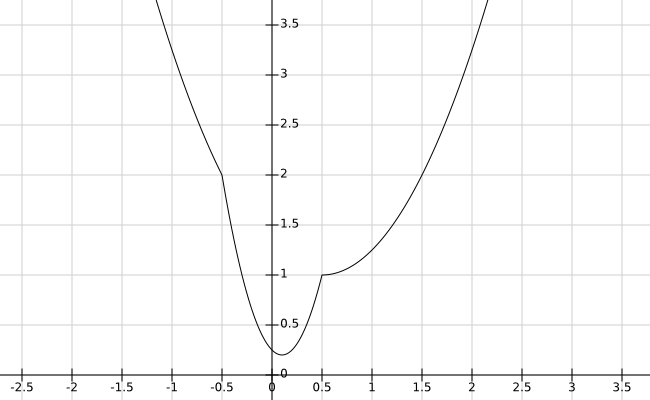
\includegraphics[width=\textwidth]{img/f_1.png}
                            \caption{$(x-\frac{1}{2})^{2} + \min(4x^{2}, 1)$}
                        \end{framed}
                    \end{subfigure}
                    \begin{subfigure}[b]{0.49\textwidth}
                        \begin{framed}
                            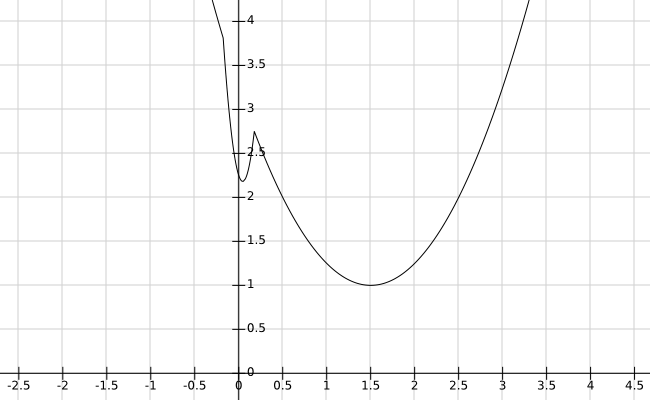
\includegraphics[width=\textwidth]{img/f_2.png}
                            \caption{$(x-\frac{3}{2})^{2} + \min(32x^{2}, 1)$}
                        \end{framed}
                    \end{subfigure}
                    \begin{subfigure}[b]{0.49\textwidth}
                        \begin{framed}
                            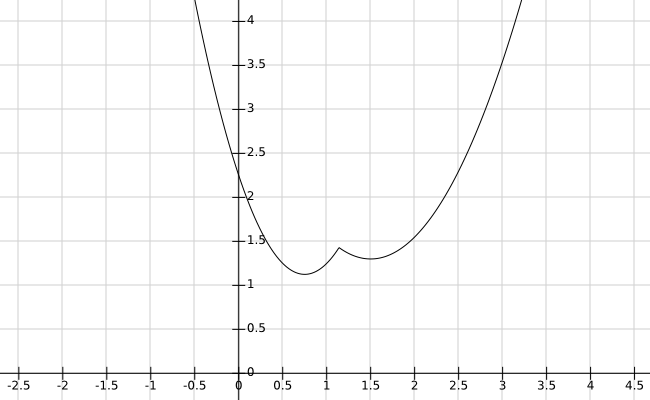
\includegraphics[width=\textwidth]{img/f_4.png}
                            \caption{$(x-\frac{3}{2})^{2} + \min(x^{2}, 1.3)$}
                        \end{framed}
                    \end{subfigure}
                    \begin{subfigure}[b]{0.49\textwidth}
                        \begin{framed}
                            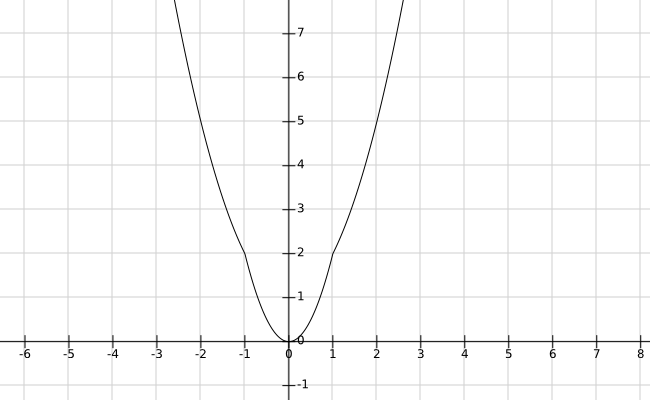
\includegraphics[width=\textwidth]{img/f_5.png}
                            \caption{$x^{2} + \min(x^{2}, 1)$}
                        \end{framed}
                    \end{subfigure}
                    \caption[Plot of the objective function within a minimum function.]{It happens, like in (a) or (d), that the objective function of the minimization problem only attains one minimum. In (c) we have two minima, but the global minimum is attained, where $|\tilde{x}_{i,j}| \le \sqrt{\frac{\nu}{\lambda}(1 + 2\gamma\lambda)}$. In (b), the global minimum is attained in the region, in which $|\tilde{x}_{i,j}| > \sqrt{\frac{\nu}{\lambda}(1 + 2\gamma\lambda)}$.}
                    \label{fig:objective_function}
                % \end{framed}
            \end{figure}

            According to \cite{Strekalovskiy-Cremers-eccv14}, there exists no theorem of convergence for this framework. Despite that fact, they show the boundedness of $u^{n}$ in the piecewise smooth case, meaning $\lambda < \infty$. This is summarized in the following proposition.
            \begin{proposition}
                The sequence $(u^{n}, p^{n})$ generated by algorithm \ref{alg:realtime_primal_dual_algorithm} is bounded and thus compact for $\lambda < \infty$, for instance it has a convergent subsequence.
            \end{proposition}

            The proof can be found in the supplementary material of \cite{Strekalovskiy-Cremers-eccv14}. Note, that in the case of this suggested framework, we also followed \cite{Strekalovskiy-Cremers-eccv14} with their proposed stopping criterion, evaluating once every ten iterations
                \begin{equation}
                    ||u^{n+1} - u^{n}|| \le \varepsilon,
                    \label{eq:stop_realtime_model}
                \end{equation}
            with $\varepsilon = 5 \cdot 10^{-5}$ and define the underlying norm by
                $$
                    ||\tilde{u}|| := \frac{1}{|\Omega|} \sum_{k = 1}^{3} \sum_{i = 1}^{N} \sum_{j = 1}^{M} |\tilde{u}_{i,j,k}|.
                $$
            Here, $k$ resembles the number of color channels. We let $k = 1, 2, 3$, for color images. If we consider grayscaled images we have $k = 1$.\\

        % subsubsection the_proximity_operators_of_the_tvl1_model (end)

    % section the_mumford_shah_functional (end)

    In this chapter we provided a framework to solve variational problems, as well as a possibility to minimize the Mumford-Shah functional. Applying this framework to images and compare the results is part of chapter \ref{cha:applications_to_imaging}. First, we want to show a second approach to minimize the Mumford-Shah functional.

% chapter convex_optimization_of_the_rof_tvl1_and_mumford_shah_models (end)

\chapter{Minimizing the Mumford-Shah Functional} % (fold)
\label{cha:minimizing_the_mumford_shah_functional}

    As we revisit the Mumford-Shah functional, we also rewrite definition \ref{def:the_mumford_shah_functional} to be consistent with the publication of Pock, Cremers, Bischof and Chambolle in \cite{Pock-et-al-iccv09}, which we mainly follow in this chapter. If other results are taken into account, we make this clear.

    \begin{definition}[Mumford-Shah Functional] % (fold)
    \label{def:the_mumford_shah_functional_revisited}

        Let $\Omega \subseteq \mathbb{R}^{2}$ be a rectangular image domain. In order to approximate an input image $f: \Omega \longrightarrow [0, 1]$ in terms of a piecewise smooth function $u: \Omega \longrightarrow [0, 1]$, Mumford and Shah suggested to minimize the functional
            
            \begin{equation}
                E_{MS}(u) = \lambda \int_{\Omega} (f - u)^{2} dx + \int_{\Omega \setminus S_{u}} |\nabla u|^{2} dx + \nu \mathcal{H}^{1}(S_{u}),
            \label{eq:the_mumford_shah_functional_revisited}
            \end{equation}
        
        where $\lambda, \nu > 0$ are weighting parameters, $S_{u} = S^{1}_{u} \cup ... \cup S^{N}_{u}$ and $\mathcal{H}^{1}(S_{u})$ denotes the one-dimensional Hausdorff-measure of the curves in $S_{u}$.

    \end{definition}
    % definition the_mumford_shah_functional (end)

    The difference to chapter \ref{cha:the_rof_tvl1_and_mumford_shah_functional} is, that we interchanged the set $K = K_{1} \cup ... \cup K_{N}$ with $S_{u} = S^{1}_{u} \cup ... \cup S^{N}_{u}$ and instead of computing $|K|$, we use the more general notation of measure theory. In the case, where $u \in \Omega \subseteq \mathbb{R}^{2}$, the one-dimensional Hausdorff-measure of $S_{u}$ is nothing but $|S_{u}|$. Another difference to definition \ref{def:the_mumford_shah_functional} is the parameter $\lambda$, which handles the tradeoff between the data fidelity term and the first term in the regularizer. It is swapped and controls now the term where the image $f$ enters the functional. As mentioned in the previous chapter, this functional is non-convex. The idea to derive a convex saddle-point representation of the Mumford-Shah functional is to make use of some results presented by Alberti, Bouchitte and Dal Maso. They applied convex relaxation techniques to approximate the Mumford-Shah functional by a convex maximization problem.

    \section{Convex Relaxation} % (fold)
    \label{sec:convex_relaxation}

        In order to state a convex relaxed model, we need to introduce the characteristic or level set function.

        \begin{definition}
        \label{def:characteristic_function}
            Let $\Omega \subseteq \mathbb{R}^{2}$ denote the image plane and let $u \in SBV(\Omega)$. The upper level sets of $u$ are denoted by the characteristic function $\mathds{1}_{u}: \Omega \times \mathbb{R} \longrightarrow \{ 0, 1 \}$ of the subgraph of $u$:
                \begin{equation}
                    \mathds{1}_{u}(x, t) =
                        \left\{
                            \begin{array}{l l}
                                1, & \quad \text{if $t < u(x)$}, \\
                                0, & \quad \text{else}.
                            \end{array}
                        \right.
                \label{eq:characteristic_function}
                \end{equation}
        \end{definition}

        In figure \ref{fig:characteristic_function} one can see an example with a characteristic function in $\mathbb{R}^{2}$ for a function $u \in SBV(\Omega)$. So, for a one-dimensional signal $u(x)$ the characteristic function becomes two-dimensional. In our case, as we consider two-dimensional images, the characteristic function adds another label space and we then act in a three-dimensional space.

        \begin{figure}[!ht]
            \centering
            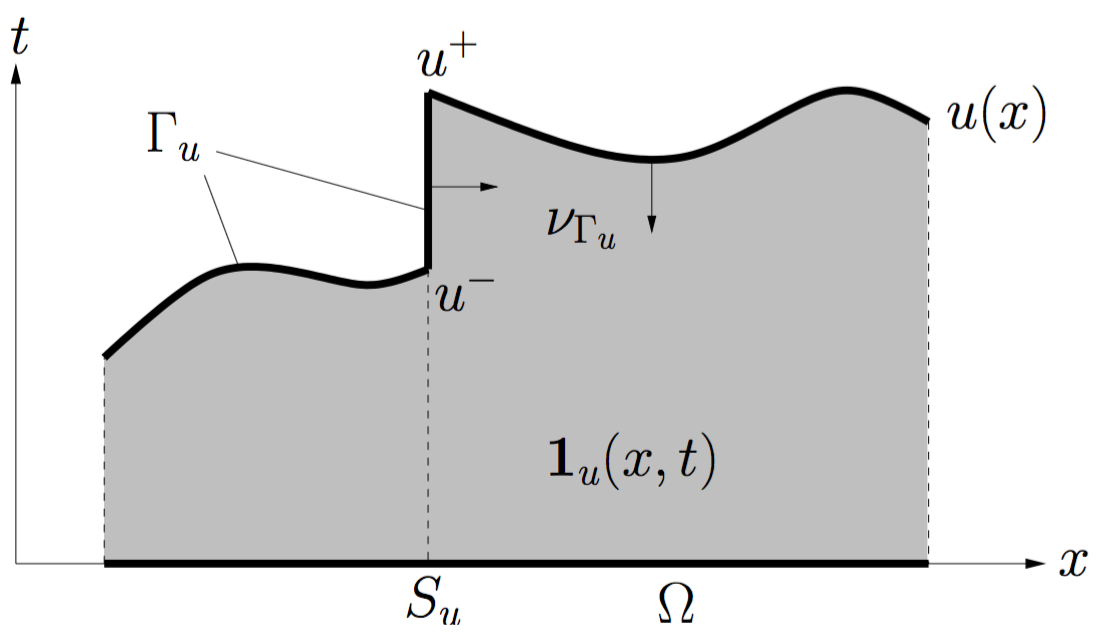
\includegraphics[width=0.7\textwidth]{img/char_func.png}
            \caption[Characteristic Function of a SBV function.]{\label{fig:characteristic_function} This picture (taken from \cite{Pock-et-al-iccv09}) shows the characteristic function $\mathds{1}_{u}(x, t)$ of a function $u(x) \in SBV(\Omega)$.}
        \end{figure}

        The gray shaded area is the part where $\mathds{1}_{u}(x, t) = 1$. Otherwise, the characteristic function is set to zero. The upper interface of the gray domain is denoted by $\Gamma_{u}$. This set is the set which holds all parts of the function $u(x)$ and each curve $S_{u}$ connecting the points $u^{-}$ and $u^{+}$. Additionally, the notation $\nu_{\Gamma_{u}}$ denotes the normals on $\Gamma_{u}$.

        Using $\mathds{1}_{u}(x, t)$, one can find in \cite{Alberti-et-al-lnss} and \cite{Alberti-et-al-cvpde} the proposed method of Alberti, Bouchitte and Dal Maso, to approximate the Mumford-Shah energy by a convex maximization problem. For a proof of this concept we refer to these two publications. We state this theorem in the fashion of \cite{Pock-et-al-iccv09}.

        \begin{theorem}[Convex Relaxation of the Mumford-Shah Functional]
        \label{convex_relaxation_of_the_mumford_shah_functional}
            For a function $u \in SBV(\Omega)$ the Mumford Shah functional can be written as
                \begin{equation}
                    E(u) = \sup_{\varphi \in K} \int_{\Omega \times \mathbb{R}} \varphi D\mathds{1}_{u}, \label{eq:convex_relaxed_ms}
                \end{equation}
            with a convex set
                \begin{eqnarray}
                    K = \bigg\{ \varphi \in C^{0}(\Omega \times \mathbb{R}, \mathbb{R}^{3}) &:& \varphi^{t}(x, t) \ge \frac{\varphi^{x}(x,t)^{2}}{4} - \lambda(t - f(x))^{2}, \\
                    &&\bigg| \int^{t_{2}}_{t_{1}} \varphi^{x}(x,s)ds \bigg| \le \nu \bigg\}, \label{eq:set_k_continuous}
                \end{eqnarray}
            where the inequalities in the definition of $K$ hold for all $x \in \Omega$ and for all $t, t_{1}, t_{2} \in \mathbb{R}$.
        \end{theorem}

        \begin{remark}
            \begin{itemize}
                \item In the theorem we used, that we represent the vector $\varphi$ by $\varphi(x, t) = \left( \varphi^{x}(x,t), \varphi^{t}(x,t) \right)^{T}$, where $\varphi(x,t) \in \mathbb{R}^{3}$, $\varphi^{x}(x,t) \in \mathbb{R}^{2}$ and $\varphi^{t}(x,t) \in \mathbb{R}$.
                \item The idea to approximate the Mumford-Shah functional is, to maximize the flux of a vector field $\varphi$ through the interface $\Gamma_{u}$. The advantage of this technique is, to get a convex representation of the Mumford-Shah functional and for this we derive in the following a convex saddle-point formulation. Then we can - again - make use of the primal-dual algorithm to solve the optimization problem.
            \end{itemize}
        \end{remark}

        Our goal is to minimize \ref{eq:convex_relaxed_ms}. We seek to solve
            $$
                \min_{u} E(u) = \min_{u} \left( \sup_{\varphi \in K} \int_{\Omega \times \mathbb{R}} \varphi D\mathds{1}_{u} \right),
            $$
        but, substitute $\mathds{1}_{u}$ by a function
            \begin{equation}
                v(x, t): \Omega \times \mathbb{R} \longrightarrow [0, 1] \,\, \textnormal{and} \,\, \lim_{t \rightarrow -\infty} v(x, t) = 1, \, \, \, \lim_{t \rightarrow +\infty} v(x, t) = 0,
            \label{eq:generic_functions}
            \end{equation}
        to compute the minimal energy of the Mumford-Shah functional. Overall, we are going to face the following convex optimization problem:
            \begin{equation}
                \min_{v \in [0, 1]} \sup_{\varphi \in K} \langle v, D\varphi \rangle = \min_{v \in [0, 1]} \sup_{\varphi \in K} \int_{\Omega \times \mathbb{R}} \varphi Dv.
                \label{eq:continous_saddle_point_problem}
            \end{equation}

        According to \cite{Pock-et-al-iccv09} there is no proof, that finding an optimal pair $(v^{\ast}, \varphi^{\ast})$ for the optimization problem \ref{eq:continous_saddle_point_problem} leads to the global minimizer of equation \ref{eq:the_mumford_shah_functional_revisited}. Further, they state that only if $v^{\ast}$ is binary one gets indeed the global minimum of the Mumford-Shah functional. Despite that fact, solving equation \ref{eq:continous_saddle_point_problem} leads to high-quality approximations $u$ of an input image $f$.

        In the next section we consider the optimization problem \ref{eq:continous_saddle_point_problem} in the discrete version. Additionally, we propose the corresponding operators and compute the proximity operators.

    % section convex_relaxation (end)

    \section{Discrete Setting} % (fold)
    \label{sec:discrete_setting_ms}

        Using the characteristic function and substitute it by the function $v$ means, that we are adding an additional space to our two dimensional image domain. This extra label space needs to be considered in the discrete setting. In \cite{Pock-et-al-iccv09} they consider $\Omega = [0, 1]^{2}$ and for that the subgraph of $u$ to be in $[0, 1]^{3}$. This would imply that we discetize these two spaces by adding a step-size $h$, where for instance $h_{N} = \frac{1}{N}$ or $h_{M} = \frac{1}{M}$. Further, they consider all their operators without having this additional step-size. To be not confusing, we propose all our spaces and operators without a step size. Then the image domain is $\Omega = \{1, 2, ..., N\} \times \{1, 2, ..., M\}$ and the subgraph of the function $u: \mathbb{R}^{2} \longrightarrow [0, 1]$ is defined in the cube $\Omega \times \{1, 2, ..., S\}$. In this discrete setting we define the pixel grid $\mathcal{G}$ with size $N \times M \times S$ and the following notation
            $$
                \mathcal{G} = \bigg\{ (i , j , k ): i = 1, 2, ..., N, j = 1, ..., M, k = 1, 2, ..., S \bigg\},
            $$
        where $i, j, k$ are the discrete locations of each voxel. For a reformulation of \ref{eq:continous_saddle_point_problem} we also need to define the corresponding discrete versions of $v, \varphi$. So, let $u \in X: \mathcal{G} \longrightarrow [0, 1]$ and $p \in Y: \mathcal{G} \longrightarrow \mathbb{R}^{3}$ be the discrete versions of the continous functions in equation \ref{eq:continous_saddle_point_problem}, where $u$ corresponds to $v$ and $p$ to $\varphi$. If we replace the inner-product for infinite dimensions in equation \ref{eq:continous_saddle_point_problem} by the inner-product for finite dimensions, we are going to face the saddle-point problem
            \begin{equation}
                \min_{u \in C} \max_{p \in K} \langle Au, p \rangle.
            \label{eq:mumford_shah_saddle_point_problem}
            \end{equation}
        This notation looks now familiar to us. Here, $A$ is the linear operator, earlier denoted with $K$. The set $C$ of the minimization is defined as
            \begin{equation}
                C = \{ u \in X: u(i,j,k) \in [0,1], u(i, j, 1) = 1, u(i, j, S) = 0 \}.
            \end{equation}
        To take the limits of the function $v$ into account in its discrete version $u$, we set the values in the first label space to $1$ and those in the S-th label space to $0$. We also model in the set $C$, that the approximation $u$ maps into $[0, 1]$.
        The discrete version of the set $K$ from equation \ref{eq:set_k_continuous} has the following representation:
            \begin{eqnarray}
                K = \{ p = (p^{x}, p^{t})^{T} \in Y &:& p^{t}(i,j,k) \ge \frac{||p^{x}(i,j,k)||_{2}^{2}}{4} - \lambda(\frac{k}{S} - f(i,j))^{2}, \label{eq:local_constraint} \\
                &&\left| \sum_{k_{1} \le k \le k_{2}} p^{x}(i,j,k) \right| \le \nu \}, \label{eq:non_local_constraint}
            \end{eqnarray}
        whereas we define $p^{x}(i,j,k) := (p^{1}(i,j,k), p^{2}(i,j,k))^{T}$ and $p^{t}(i,j,k) := p^{3}(i,j,k)$ for a $p(i,j,k) \in \mathbb{R}^{3}$. For this, $p^{x} \in \mathbb{R}^{N \cdot M \cdot S \cdot 2}$ and $p^{t} \in \mathbb{R}^{N \cdot M \cdot S}$. The constraint in equation \ref{eq:local_constraint} goes pointwise for all $(i, j, k) \in \mathcal{G}$. The second constraint is more involved, since the constraint in \ref{eq:non_local_constraint} holds for all $i = 1, ..., N$, $j = 1, ..., M$ and all possible combinations $(k_{1}, k_{2})$ for all $k_{1}, k_{2} = 1, ..., S$. What looks like having a set $K$ with two constraints, turns out that the set $K$ is an intersection of a couple of convex sets. Namely, one has that for a fixed voxel $(i, j, k)$ one can compute $\frac{S (S - 1)}{2} + S + 1$ many convex sets. This number rises from the fact, that taking into account all possible combinations $(k_{1}, k_{2})$ over all levels $S$ and adding the local-constraint, yields
            $$
                \binom{S}{2} + S + 1 = \frac{n!}{k! \cdot (n-k)!} + S + 1 = \frac{S(S-1)}{2} + S + 1.
            $$
        The large amount of several convex sets will lead us to a long run-time in the suggested framework in \cite{Pock-et-al-iccv09}. Before we discuss this in detail, we first continue with the definitions of the discrete setting.

        \begin{remark}
            In addition to discretize the variable $t$ in \ref{eq:set_k_continuous} one gets $\frac{k}{S}$ in the discrete version of \ref{eq:local_constraint}. Note, that $t$ is a value in the continuous setting, which determines at which point the characteristic function vanishes, i.e. is set to zero. The bound on the norm $L$ depends on the discrete gradient operator, like in propositions \ref{prop:bound_on_the_norm} or \ref{prop:bound_on_the_norm_ms}. In \cite{Pock-et-al-iccv09} they proposed to set the discrete version of $t$ to $\frac{k}{L}$, which is a mistake.
        \end{remark}

        We further need to define the representation of the linear operator $A$. It is the same as found in section \ref{sec:discrete_setting}, namely the discrete gradient operator, but extended to the additional label space.

        \begin{definition}[Discrete gradient operator] % (fold)
        \label{def:discrete_gradient_operator_ms}

            We define the discrete gradient of $u \in X$ by $\nabla u = ((\partial_{i}u)_{i,j,k}, (\partial_{j}u)_{i,j,k}, (\partial_{k}u)_{i,j,k})^{T}$ using forward differences with Neumann boundary conditions, i.e
                \begin{eqnarray}
                    &(\partial_{i}u)_{i,j,k} =&
                        \begin{dcases*}
                            u_{i+1, j, k} - u_{i, j, k} & \textnormal{if $i < N$} \\
                            0 & \textnormal{if $i = N$}
                        \end{dcases*}
                    \notag
                    (\partial_{j}u)_{i, j, k} =
                        \begin{dcases*}
                            u_{i, j+1, k} - u_{i, j, k} & \textnormal{if $j < M$} \\
                            0 & \textnormal{if $j = M$}
                        \end{dcases*}
                    \notag \\
                    &(\partial_{k}u)_{i, j, k} =&
                        \begin{dcases*}
                            u_{i, j, k+1} - u_{i, j, k} & \textnormal{if $k < S$} \\
                            0 & \textnormal{if $k = S$}
                        \end{dcases*}
                    \notag
                \end{eqnarray}

        \end{definition}
        % definition discrete_gradient_operator (end)

        Again we have $\nabla^{T}: Y \longrightarrow X$ as the discrete divergence operator, with $-\nabla^{T} = \textnormal{div}$, as seen before.

        \begin{definition}[Discrete divergence operator] % (fold)
        \label{def:discrete_divergence_operator_ms}

            We define the discrete divergence of $p \in Y$ by $\nabla^{T} p = (\partial_{i}p^{1})_{i, j, k} + (\partial_{j}p^{2})_{i, j, k} + (\partial_{k}p^{3})_{i, j, k}$ using backward differences with Dirichlet boundary conditions, i.e
                \begin{eqnarray}
                    &(\partial_{i}p^{1})_{i, j, k} =&
                        \begin{dcases*}
                            p^{1}_{i, j, k} - p^{1}_{i-1, j, k} & \textnormal{if $1 < i < N$} \\
                            p^{1}_{i, j, k} & \textnormal{if $i = 1$} \\
                            -p^{1}_{i-1, j, k} & \textnormal{if $i = N$}
                        \end{dcases*}
                    \notag
                    (\partial_{j}p^{2})_{i, j, k} =
                        \begin{dcases*}
                            p^{2}_{i, j, k} - p^{2}_{i, j-1, k} & \textnormal{if $1 < j < M$} \\
                            p^{2}_{i, j, k} & \textnormal{if $j = 1$} \\
                            -p^{2}_{i, j-1, k} & \textnormal{if $j = M$}
                        \end{dcases*}
                    \notag \\
                    &(\partial_{k}p^{3})_{i, j, k} =&
                        \begin{dcases*}
                            p^{3}_{i, j, k} - p^{3}_{i, j, k-1} & \textnormal{if $1 < k < S$} \\
                            p^{3}_{i, j, k} & \textnormal{if $k = 1$} \\
                            -p^{3}_{i, j, k-1} & \textnormal{if $k = S$}
                        \end{dcases*}
                    \notag
                \end{eqnarray}

        \end{definition}
        % definition discrete_gradient_operator (end)

        \begin{proposition}[Bound on the norm of $\nabla$] % (fold)
            \label{prop:bound_on_the_norm_ms}

            The bound on the norm of the proposed discrete linear operator is given by
                $$
                    L^{2} = ||\nabla||^{2} = ||\nabla^{T}||^{2} \le 12.
                $$
        \end{proposition}
        % proposition bound_on_the_norm (end)

        \begin{proof}
        	The proof is the same as in section \ref{sec:discrete_setting} by adding the additional discretization variable $p^{3}_{i,j,k}$.\qed
        \end{proof}

    % section discrete_setting (end)

    \section{Primal and Dual Formulation} % (fold)
    \label{sub:primal_and_dual_formulation}

    	Recalling equation \ref{eq:mumford_shah_saddle_point_problem} and setting $A = \nabla$, we have that a minimizer of the Mumford-Shah functional can be computed by solving
    		\begin{equation}
    			\min_{u \in C} \max_{p \in K} \langle \nabla u, p \rangle = \min_{u \in C} \max_{p \in K} \langle \nabla u, p \rangle - \delta_{K}(p) + \delta_{C}(u).
    			\label{eq:primal_dual_mumford_shah}
    		\end{equation}

    	As in the chapter before, we first want to formulate this saddle-point problem in the primal and the dual version. Afterwards, we want to compute the proximity operators for the corresponding functions $G(u) = \delta_{C}(u)$ and $F^{\ast}(p) = \delta_{K}(p)$.

        First we compute the primal formulation of the Mumford-Shah model. Therefore, it is left to determine $F$ from $F^{\ast}$. Assume the function $F(g)$ to be convex, then the Legendre-Fenchel conjugate is given by
            $$
                F^{\ast}(p) = \sup_{g \in X} \left( \langle g, p \rangle - F(g) \right).
            $$
        For $F$ convex we observe on the other hand, with equality $F^{\ast\ast} = F$ holding, that
            $$
                F(g) = \sup_{p \in Y} \left( \langle g, p \rangle - F^{\ast}(p) \right) = \sup_{p \in Y} \left( \langle g, p \rangle - \delta_{K}(p) \right).
            $$
        We want to compute $F(g)$ and show that the function $F$ is indeed convex. Computing $F$ means solving the convex problem
            $$
                \sup_{p \in Y} \left( \langle g, p \rangle - \delta_{K}(p) \right) = \sup_{p \in K} \langle g, p \rangle.
            $$
        Assume, $\hat{p} \in -\min\limits_{p \in K} \langle p, g \rangle$, then we have with proposition \ref{prop:zero_element_of_subgradient}
            $$
                \max_{p \in K} \langle g, p \rangle \Longleftrightarrow -\min\limits_{p \in K} \langle p, g \rangle \Longleftrightarrow 0 \in \partial_{p} \left( \langle g, \hat{p} \rangle \right) \Longleftrightarrow 0 \in g \Longrightarrow g = 0.
            $$
        But, this means, if $g = 0$ then $F(g) = 0$. If $g < 0$ holds, then the only choice to attain a maximal value is to let $p$ go to $- \infty$. But if $g > 0$ then $p \to \infty$, reversely. For an arbitray argument of $F$, we set
            $$
                F(u) =
                    \begin{dcases*}
                        u & \textnormal{if $u = 0$,} \\
                        \infty & \textnormal{else.}
                    \end{dcases*}
            $$
        This is nothing but the indicator function of a single point and for this a convex function. Then for the primal formulation we get
            \begin{eqnarray}
                \min_{u \in X} F(\nabla u) + G(u) &\Longleftrightarrow& \min_{u \in C} G(u) \notag \\
                &\textnormal{s.t.}& \,\,\, \nabla u = 0. \notag
            \end{eqnarray}

    	Finally, we also want to evaluate the dual formulation of the Mumford-Shah saddle-point problem. We need to compute the Legendre-Fenchel conjugate of $G$. Since $G$ is the indicator function of the set $C$ we can make use of example \ref{ex:legendre_fenchel_conjugate_example} 1. and observe
            $$
                G^{\ast}(p) = \delta^{\ast}_{C}(p) = \sup\limits_{u \in C} \langle p, u \rangle,
            $$
        which is the support function of $C$. Overall, with $K^{\ast} = \nabla^{T} = -\textnormal{div}$ we obtain the dual problem by
        	\begin{equation}
        		\max_{p \in Y} -(G^{\ast}(-K^{\ast}p) + F^{\ast}(p)) = \max_{p \in Y} -(\sup\limits_{u \in C} \langle -\nabla^{T}p, u \rangle + \delta_{K}(p)) = \max_{p \in K} -(\sup\limits_{u \in C} \langle \textnormal{div}(p), u \rangle).
        	\label{eq:dual_mumford_shah_old}
        	\end{equation}
        Now, assume that after the n-th iteration of the primal-dual algorithm we computed a $p^{n} \in K$. Then we can rewrite equation \ref{eq:dual_mumford_shah_old} into
            \begin{equation}
                -\max_{u \in C} \langle \nabla^{T}p^{n}, u \rangle = \min_{u \in C} \langle \nabla^{T}p^{n}, u \rangle.
            \label{eq:dual_mumford_shah}
            \end{equation}
        
        It is left to compute the proximity operators. Since, the proximity operator of the indicator function is a euclidean projection onto the corresponding set, we need to describe how a projection on $C$ and $K$ can be derived. But first, we rewrite the primal-dual algorithm \ref{alg:primal_dual_algorithm} to be consistent with \cite{Pock-et-al-iccv09}.

    		\begin{algorithm}\label{alg:primal_dual_cremers}
                Choose $(u^{0}, p^{0}) \in C \times K$ and let $\bar{u}^{0} = u^{0}$. We choose $\tau, \sigma > 0$. Then, we let for each $n \ge 0$
                    \begin{equation}
                        \left\{ 
                            \begin{array}{l l}
                              p^{n+1} = \Pi_{K} (p^{n} + \sigma K \bar{u}^{n}) \\
                              u^{n+1} = \Pi_{C} (u^{n} - \tau K^{*} p^{n+1}) \\
                              \bar{u}^{n+1} = 2u^{n+1} - u^{n}.
                            \end{array}
                        \right.
                    \end{equation}
            \end{algorithm}

        Here we denote $\Pi_{K}$ and $\Pi_{C}$ as the (euclidean) projections on the sets $K$ and $C$. How we compute such projections will be discussed in the next section.

    \section{Projection onto the sets $C$ and $K$} % (fold)
    \label{sec:projection_onto_the_sets_C_and_K}

        We start with the projection onto the set $C$ and go on by providing an algorithm to project onto the set $K$.

        \subsection{Projection onto $C$}

        The projection onto $C$ can efficiently be computed. By definition of the proximity operator we have
            $$
                u = \arg\min_{u \in X} \frac{||u-\tilde{u}||_{2}^{2}}{2} + \tau \delta_{C}(u) = \arg\min_{u \in C} \sum_{i = 1}^{N} \sum_{j = 1}^{M} \sum_{k = 1}^{S} \frac{u_{i,j,k} - \tilde{u}_{i,j,k})^{2}}{2} = \Pi_{C}(\tilde{u}).
            $$
        As this projection goes pointwise, assume that $\tilde{u}_{i,j,k} \in C$ for a voxel $(i,j,k)$. Then the best choice for $u_{i,j,k}$ is to set $u_{i,j,k} = \tilde{u}_{i,j,k}$, since the term  is then equal to zero, for which the quadratic function is minimal. On the other hand, if $\tilde{u}_{i,j,k} \notin C$, the euclidean distance to $C = [0, 1]$ is the shortest distance $\tilde{u}_{i,j,k}$ onto the bound of $C$. This means if $\tilde{u}_{i,j,k} < 0$ then the shortest distance from $\tilde{u}_{i,j,k}$ to $C$ is to set $u_{i,j,k} = 0$. Reversely, if $\tilde{u}_{i,j,k} > 1$ then the euclidean distance to $C$ is given by setting $u_{i,j,k} = 1$. This idea is also illustrated in figure \ref{fig:projection_onto_c}. For an arbitrary intervall $[a, b]$ we have the following algorithm:

        \begin{algorithm}[Clipping]
            The projection of a point $u^{n} \in \mathbb{R}$ onto the intervall $[a, b]$, where $a,b \in \mathbb{R}$ and $a < b$ is given by
                \begin{equation}
                    u^{n+1} = \min\{b, \max \{ a, u^{n} \} \}
                    \label{eq:clipping}
                \end{equation}
        \end{algorithm}

        \begin{figure}[!ht]
            \centering
            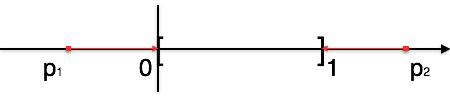
\includegraphics[width=0.9\textwidth]{img/projection_onto_c.png}
            \caption[Clipping onto the set $C$.]{\label{fig:projection_onto_c} A point $p_{1} < 0$ is clipped to $0$, whereas a point $p_{2} > 1$ is clipped to $1$.}
        \end{figure}

        \begin{remark}
            \label{rem:clipping}
            \begin{itemize}
                \item By projecting onto $C$, we also need to take care about the limits in \ref{eq:generic_functions}. For that we set $u(i, j, 1) = 1$ and $u(i, j, S) = 0$ in each projection.
                \item In the case of our framework - acting in a discrete cube $\mathcal{G}$ - equation \ref{eq:clipping} can be regarded as
                    $$
                        u^{n+1}_{i,j,k} = \min\{1, \max \{ 0, u^{n}_{i,j,k} \} \},
                    $$
                for all $i = 1, ..., N$, $j = 1, ..., M$ and $k = 1, ..., S$.
            \end{itemize}
        \end{remark}

        \subsection{The projection onto $K$} % (fold)
        \label{sub:the_projection_onto_K}

            The projection onto $K$ is more involved, since $K$ takes into account local and non-local constraints. In other words, the set $K$ is an intersection of several convex sets. The projection onto the intersection of convex sets can be done by Dykstra's projection algorithm. The idea behind this algorithm is to project a point $x$ onto each set seperately in an iteration step $n$. Then as $n \to \infty$ the algorithm finds a point $\hat{x}$ in $K$, for which the distance $||x - \hat{x}||_{2}$ is minimal. The full scheme was first proposed by Boyle and Dykstra in \cite{dykstra-et-al-aors14}, where one can also find a proof of convergence for the proposed algorithm. We follow the notation of Cremers and Kolev in \cite{Cremers-Kolev-pami11}.

            \begin{algorithm}
            \label{alg:dykstra}
                Consider $P$ convex sets $X_{i}$ with $\mathbb{R}^{n} \ni X = X_{1} \cap X_{2} \cap ... \cap X_{P}$. Let $\Pi_{i}$ denote the projection onto the i-th set for $i = 1, ..., P$. And let $u_{c} \in \mathbb{R}^{n}$ be the current estimate with $u_{c} \notin X$, $u_{i}^{k} \in \mathbb{R}^{n}$ for $i = 0, ..., P$ and $v_{i}^{k} \in \mathbb{R}^{n}$ for $i = 1, ..., P$ and $k = 1, 2, ...$, where $k$ denotes the number of iterations. Then the algorithm finds the (only) $u^{\ast} \in X$.
                For $k = 1, 2, ...$ set $u^{0}_{P} = u_{c}$ and $v^{0}_{i} = 0$ for all $i = 1, ..., P$. Then iterate until convergence (e.g. $||u_{0}^{k} - u_{P}^{k}||_{2} \le \varepsilon$ with $\varepsilon$ small):
                \begin{eqnarray}
                    &u_{0}^{k} = &u_{P}^{k-1}, \notag \\
                    &\textnormal{for} \,\, &i = 1, 2, ..., P: \notag \\
                    &&u_{i}^{k} = \Pi_{i}(u_{i-1}^{k} - v_{i}^{k-1}), \notag \\
                    &&v_{i}^{k} = u_{i}^{k} - (u_{i-1}^{k} - v_{i}^{k-1}). \notag
                \end{eqnarray}
            \end{algorithm}
            
            Now, that we know, how the projection onto the entire set $K$ can be established, we need to discuss how a projection onto the subsets of $K$ can be computed.

        % subsection the_projection_onto_K (end)

        \subsection{Decomposition of $K$} % (fold)
        \label{sub:decomposition_of_K}
            
            We will decompose the set $K$ into sets $K_{p}$ and $K_{nl}$, where the first resembles the local, or more precisely, a parabola constraint and the second corresponds to the non-local constraint. Overall, we have $K = K_{p} \cap K_{nl}$ with
                $$
                    K_{p} = \bigg\{ p^{t}(i, j, k) \ge \frac{||p^{x}(i, j, k)||^{2}}{4} - \lambda(\frac{k}{S} - f(i,j))^{2} \bigg\},
                $$
            for all $i = 1, ..., N$, $j = 1, ..., M$ and $k = 1, ..., S$. And for the non-local constraint we have
                $$
                    K_{nl} = \bigg\{ \left| \sum_{k_{1} \le k \le k_{2}} p^{x}(i, j, k) \right| \le \nu \bigg\},
                $$
            again for all $i = 1, ..., N$ and $j = 1, ..., M$, and additionally for all combinations $(k_{1}, k_{2})$ with $1 \le k_{1} \le k_{2} \le S$. We will now deduce the projection onto these two sets. Let us start with the projection onto the parabola constraint.

        % subsection decomposition_of_K (end)

        \subsection{Projection onto $K_{p}$}

            Since, the projection onto the set $K_{p}$ goes pointwise we want to drop the indices $(i, j, k)$. Note that we do not necessarily need that $p^{x}$ is an element of $\mathbb{R}^{2}$. The following derivation holds for a larger class of problems, namely having $p^{x} \in \mathbb{R}^{n}$. Let $\alpha > 0$, $p^{x} \in \mathbb{R}^{n}$, $p^{t} \in \mathbb{R}$ and $p = (p^{x}, p^{t})^{T} \in \mathbb{R}^{n} \times \mathbb{R}$. Assume that $p_{0}^{t} < \alpha ||p_{0}^{x}||_{2}^{2}$ holds for a point $p_{0} \in \mathbb{R}^{n}\times\mathbb{R}$. Then the projection of $p_{0}$ onto the parabola $\alpha ||p_{0}^{x}||_{2}^{2}$ can be written as the following minimization problem:
                \begin{eqnarray}
                    &\min\limits_{p \in \mathbb{R}^{n} \times \mathbb{R}}& \frac{1}{2} ||p - p_{0}||_{2}^{2} \notag \\
                    &\textnormal{subject to}& p^{t} \ge \alpha||p^{x}||_{2}^{2}. \notag
                \end{eqnarray}
            To find the solution of this optimization problem we introduce a Lagrange Multiplier $\mu \in \mathbb{R}$ and define the Lagrangian as
                $$
                    \mathcal{L}(p, \mu) = \frac{||p - p_{0}||_{2}^{2}}{2} - \mu \left( p^{t} - \alpha||p^{x}||_{2}^{2} \right).
                $$
            We are seeking to minimize $\mathcal{L}(p, \mu)$ over all $p$ and $\mu$. The minimization problem we consider is convex, because the cost function is convex, the inequality constraint is convex and the feasible set $\mathbb{R}^{n} \times \mathbb{R}$ is also convex. For that, we know that computing a critical point of the Lagrangian function $\mathcal{L}$ also leads to a global optimum of the optimization problem itself. We compute a critical point by
                \begin{equation}
                    \nabla \mathcal{L}(p, \mu) =
                    \begin{pmatrix}
                        \partial_{p^{x}} \mathcal{L}(p, \mu) \\
                        \partial_{p^{t}} \mathcal{L}(p, \mu) \\
                        \partial_{\mu} \mathcal{L}(p, \mu)
                    \end{pmatrix} = 
                    \begin{pmatrix}
                        p^{x} - p_{0}^{x} + \mu 2 \alpha p^{x} \\
                        p^{t} - p_{0}^{t} - \mu \\
                        p^{t} - \alpha||p^{x}||_{2}^{2}
                    \end{pmatrix}
                    = 0. \label{eq:linearSystem}
                \end{equation}
            This means, we need to solve a linear system. In the first equation we get
                \begin{equation}
                    p_{0}^{x} = (\mu 2 \alpha + 1) p^{x} \Longleftrightarrow p^{x} = \frac{p_{0}^{x}}{\mu 2 \alpha + 1}, \label{eq:1stequ}
                \end{equation}
            and the second equation leads us to
                \begin{equation}
                    p^{t} = p_{0}^{t} + \mu. \label{eq:2ndequ}
                \end{equation}
            In the following we discuss two different possibilities how the system \ref{eq:linearSystem} can be solved.
            \begin{enumerate}
                \item Plugging the equalities \ref{eq:1stequ} and \ref{eq:2ndequ} into the third line of equation \ref{eq:linearSystem}, we observe
                \begin{eqnarray}
                    p^{t} - \alpha||p^{x}||_{2}^{2} &\Longleftrightarrow& p_{0}^{t} + \mu - \alpha \bigg|\bigg|\frac{p_{0}^{x}}{\mu 2 \alpha + 1}\bigg|\bigg|_{2}^{2} = 0 \notag \\
                    &\Longleftrightarrow& p_{0}^{t} + \mu - \frac{\alpha}{(\mu 2 \alpha + 1)^{2}} ||p_{0}^{x}||_{2}^{2} = 0 \notag \\
                    &\overbrace{\Longleftrightarrow}^{\cdot (\mu2\alpha + 1)^{2}}& (\mu 2 \alpha + 1)^{2} p_{0}^{t} + (\mu 2 \alpha + 1)^{2} \mu - \alpha ||p_{0}^{x}||_{2}^{2} = 0 \notag \\
                    &\Longleftrightarrow& (4 \mu^{2} \alpha^{2} + 4 \mu \alpha + 1) p_{0}^{t} + 4 \mu^{3} \alpha^{2} + 4 \mu^{2} \alpha + \mu - \alpha ||p_{0}^{x}||_{2}^{2} = 0 \notag \\
                    &\Longleftrightarrow& 4 \alpha^{2} \mu^{3} + \mu^{2} (4 \alpha^{2} p_{0}^{t} + 4 \alpha) + \mu (4 \alpha p_{0}^{t} + 1) + p_{0}^{t} - \alpha ||p_{0}^{x}||_{2}^{2} = 0. \notag
                \end{eqnarray}
                To solve this, we define a function
                    $$
                        h(\mu) = 4 \alpha^{2} \mu^{3} + \mu^{2} (4 \alpha^{2} p_{0}^{t} + 4 \alpha) + \mu (4 \alpha p_{0}^{t} + 1) + p_{0}^{t} - \alpha ||p_{0}^{x}||_{2}^{2},
                    $$
                for which we are seeking for the zeroes. Computing the zeroes can efficiently be established by using Newton's algorithm
                    $$
                        \mu^{k+1} = \mu^{k} - \frac{h(\mu)}{h^{'}(\mu)},
                    $$
                for $k = 1, 2, ...$, until convergence. The first derivative of $h$ is given by
                    $$
                        h^{'}(\mu) = 12 \alpha^{2} \mu^{2} + 2 \mu (4 \alpha^{2} p_{0}^{t} + 4 \alpha) + (4 \alpha p_{0}^{t} + 1).
                    $$
                Overall, we get the update equation for a $\mu^{k+1}$ with
                    $$
                        \mu^{k+1} = \mu^{k} - \frac{4 \alpha^{2} \mu^{3} + \mu^{2} (4 \alpha^{2} p_{0}^{t} + 4 \alpha) + \mu(4 \alpha p_{0}^{t} + 1) + p_{0}^{t} - \alpha ||p_{0}^{x}||_{2}^{2}}{12 \alpha^{2} \mu^{2} + 2 \mu (4 \alpha^{2} p_{0}^{t} + 4 \alpha) + (4 \alpha p_{0}^{t} + 1)}.
                    $$
                In \cite{Chambolle-et-al-10} they suggest setting $\mu^{0} = \max \{ 0, - \frac{2 p_{0}^{t}}{3} \}$, where they state that Newton's method converges within 7-10 iterations to a quite accurate solution.\\
                The projected vector $p$ of our problem is then given by
                    $$
                        p = \left( \frac{p_{0}^{x}}{\mu 2 \alpha + 1}, p_{0}^{t} + \mu \right),
                    $$
                which we get from equations \ref{eq:1stequ} and \ref{eq:2ndequ}. We did not apply this method to our implementation, since the primal-dual algorithm will be extremley slow in the case of this framework. Having a few iterations of Newton's algorithm in each primal-dual iteration, additionally generates more overhead and for that would decelerate the program. Further, Newton's method is inexact and as it turns out, the second approach to this problem will lead to a exact solution, which can be computed within one loop of straightforward computations.
            \item For the second approach we note that \ref{eq:1stequ} and \ref{eq:2ndequ} hold and the third equation in \ref{eq:linearSystem} can be expressed by
                \begin{equation}
                    p^{t} = \alpha ||p^{x}||_{2}^{2} \Longleftrightarrow p_{0}^{t} + \mu = \alpha ||p^{x}||_{2}^{2}. \label{eq:tmp1}
                \end{equation}
            With equation \ref{eq:1stequ} we can compute the solution of $\mu$ by using
                \begin{eqnarray}
                    p^{x} = \frac{p_{0}^{x}}{\mu 2 \alpha + 1} &\Longleftrightarrow& ||p^{x}||_{2} = \bigg|\bigg| \frac{p_{0}^{x}}{1 + 2 \alpha \mu} \bigg|\bigg|_{2} \notag \\
                    &\Longleftrightarrow& ||p^{x}||_{2} = \frac{1}{1 + 2 \alpha \mu} ||p_{0}^{x}||_{2} \notag \\
                    &\Longleftrightarrow& \frac{1}{1 + 2 \alpha \mu} = \frac{||p^{x}||_{2}}{||p_{0}^{x}||_{2}} \notag \\
                    &\Longleftrightarrow& 1 + 2\alpha\mu = \frac{||p_{0}||_{2}}{||p_{x}||_{2}} \notag \\
                    &\Longleftrightarrow& 2 \alpha \mu = \frac{||p_{0}^{x}||_{2}}{||p^{x}||_{2}} - 1 \notag \\
                    &\Longleftrightarrow& \mu = \frac{1}{2 \alpha} \left( \frac{||p_{0}^{x}||_{2}}{||p^{x}||_{2}} \right) - \frac{1}{2\alpha}. \notag
                \end{eqnarray}
            We then plug the solution of $\mu$ in \ref{eq:tmp1} and observe
                \begin{eqnarray}
                    \alpha ||p^{x}||_{2}^{2} &=& p_{0}^{t} + \frac{1}{2 \alpha} \left( \frac{||p_{0}^{x}||_{2}}{||p^{x}||_{2}} \right) - \frac{1}{2\alpha} \notag \\
                    &\overbrace{\Longleftrightarrow}^{\cdot 2 \alpha ||p^{x}||_{2}}& 2 \alpha^{2} ||p^{x}||_{2}^{3} = 2 \alpha ||p^{x}||_{2} p_{0}^{t} + ||p_{0}^{x}||_{2} - ||p^{x}||_{2} \notag \\
                    &\Longleftrightarrow& 2 \alpha^{2} ||p^{x}||_{2}^{3} + 2\alpha||p^{x}||_{2} - 2\alpha p_{0}^{t} ||p^{x}||_{2} - ||p_{0}^{x}||_{2} = 0. \notag \\
                    &\Longleftrightarrow& 2 \alpha^{2} ||p^{x}||_{2}^{3} + (1 - 2 \alpha p_{0}^{t}) ||p^{x}||_{2} - ||p_{0}^{x}||_{2} = 0. \notag \\
                    &\overbrace{\Longleftrightarrow}^{\cdot 4 \alpha}& 8 \alpha^{3} ||p^{x}||_{2}^{3} + 4 \alpha (1 - 2 \alpha p_{0}^{t}) ||p^{x}||_{2} - 4 \alpha ||p_{0}^{x}||_{2} = 0. \notag \\
                    &\Longleftrightarrow& (2 \alpha ||p^{x}||_{2})^{3} + 2 (1 - 2 \alpha p_{0}^{t}) 2 \alpha ||p^{x}||_{2} - 4 \alpha ||p_{0}^{x}||_{2} = 0. \notag \\
                    &\Longleftrightarrow& t^{3} + 3bt - 2a = 0, \label{eq:cubic}
                \end{eqnarray}
            with $a = 2 \alpha ||p_{0}^{x}||_{2}$, $b = \frac{2}{3}(1 - 2 \alpha p_{0}^{t})$ and $t = 2 \alpha ||p^{x}||_{2}$.\\
            The cubic equation \ref{eq:cubic} in $t$ can efficiently be solved using the analytical formula for solving cubic equations published by J. P. McKelvey in 1984 in \cite{kelvey-ajp}.
            \end{enumerate}

            The result of this work is summarized in the following algorithm. Note, that we already computed the factors $a$ and $b$. The others follow with \cite{kelvey-ajp}.

                \begin{algorithm}
                    \label{alg:projection_on_parabola}
                    If already $p_{0}^{t} \ge \alpha ||p_{0}^{x}||_{2}^{2}$, the solution is given by $(p^{x}, p^{t}) = (p_{0}^{x}, p_{0}^{t})$. Otherwise, with $a = 2 \alpha ||p_{0}^{x}||_{2}$, $b = \frac{2}{3} (1 - 2 \alpha p_{0}^{t})$, and

                        \[
                            d =
                                \begin{dcases*}
                                    a^{2} + b^{3} & \textnormal{if $b \ge 0$}\\
                                    (a - \sqrt{-b}^{3})(a + \sqrt{-b}^{3}) & \textnormal{else,}
                                \end{dcases*}
                        \]
                    we set
                        \[
                            v =
                                \begin{dcases*}
                                    c - \frac{b}{c} \,\, \textnormal{with} \,\, c = \sqrt[3]{a + \sqrt{d}} & \textnormal{if $d \ge 0$}\\
                                    2 \sqrt{-b} \cos \left( \frac{1}{3} \arccos \frac{a}{\sqrt{-b}^{3}} \right) & \textnormal{else}.
                                \end{dcases*}
                        \]
                    If $c = 0$ in the first case, set $v = 0$. The solution is then given by
                        \[
                            p^{x} =
                                \begin{dcases*}
                                    \frac{v}{2\alpha} \frac{p_{0}^{x}}{||p_{0}^{x}||_{2}} & \textnormal{if $p_{0}^{x} \ne 0$}\\
                                    0 & \textnormal{else,}
                                \end{dcases*}
                        \]
                    and $p^{t} = \alpha ||p^{x}||_{2}^{2}$.
                \end{algorithm}

            The above method states that the projection onto the parabola can be done by one cycle of straightforward computations. The implementation of it is simple and computation time is fast. It is left to show, how we project onto $K_{nl}$.

        \subsection{Projection onto $K_{nl}$}

            This set is a combination of non-local constraints, meaning that in a fixed voxel $(i, j, k)$ we sum up for all possible combinations $k_{1} \le k \le k_{2}$ for all $k, k_{1}, k_{2} = 1, ..., S$. For that reason, we can not project pointwise. We make use of a so called soft-shrinkage scheme. Let us first present the algorithm and then give a proof of concept.

            \begin{algorithm}[Soft-Shrinkage Scheme]
            \label{alg:softshrinkage}
                Let $(p^{x}(i,j,k))^{n} \in \mathbb{R}^{2}$ for all iterations $n = 1, 2, ...$. Then the projection $(p^{x}(i,j,k))^{n+1}$ of $(p^{x}(i,j,k))^{n}$ - for a fixed pair $(k_{1}, k_{2})$ with $1 \le k_{1} \le k \le k_{2} \le S$ - is computed by:

                    \[
                        (p^{x}(i,j,k))^{n+1} =
                            \begin{dcases*}
                                (p^{x}(i,j,k))^{n} + \frac{s_{k_{1}, k_{2}} - \tilde{s}_{k_{1}, k_{2}}}{k_{2} - k_{1} + 1} & \textnormal{if $k_{1} \le k \le k_{2}$}, \\
                                (p^{x}(i,j,k))^{n} & \textnormal{else},
                            \end{dcases*}
                    \]
                where $s_{k_{1}, k_{2}}, \tilde{s}_{k_{1}, k_{2}} \in \mathbb{R}^{2}$ with
                    $$
                        \tilde{s}_{k_{1}, k_{2}} = \sum_{k_{1} \le k \le k_{2}} (p^{x}(i,j,k))^{n}
                    $$
                and
                    \[
                        s_{k_{1}, k_{2}} =
                            \begin{dcases*}
                                \tilde{s}_{k_{1}, k_{2}} & \textnormal{if $|\tilde{s}_{k_{1}, k_{2}}| \le \nu$},\\
                                \Pi_{|\cdot| \le \nu}(\tilde{s}_{k_{1}, k_{2}}) = \frac{\nu}{|\tilde{s}_{k_{1}, k_{2}}|} \tilde{s}_{k_{1}, k_{2}} & \textnormal{else}.
                            \end{dcases*}
                    \]
            \end{algorithm}

            Since, this procedure needs a clarification, we need the KKT conditions. Let us introduce these conditions by following the notation, definition and theorem of \cite{Nocedal-Wright}. We consider the optimization problem:
                \begin{equation}
                    \min_{x \in \mathbb{R}^{n}} \, f(x) \,\,\,\,\, \textnormal{subject to} \,\,\,
                    \begin{dcases*}
                        c_{i}(x) = 0 & $i \in \mathcal{E}$, \\
                        c_{i}(x) \ge 0 & $i \in \mathcal{I}$,
                    \end{dcases*}
                    \label{eq:basic_optimization_problem}
                \end{equation}
            where $f$ and for all $i \in \mathcal{E} \cup \mathcal{I}$ the functions $c_{i}$ are smooth, real-valued functions on a subset of $\mathbb{R}^{n}$. Further, $\mathcal{E}$ and $\mathcal{I}$ denote two finite sets of indices. Here, $f$ is the objective function, whereas the $c_{i}$ for $i \in \mathcal{E}$ are the equality constraints and $c_{i}$ with $i \in \mathcal{I}$ the inequality constraints. We further want to define the feasible set $\Omega$. As stated in section \ref{sec:convex_optimization_and_convex_analysis}, this set is the set of all points, which satisfy the constraints $c_{i}$ for all $i$. Then we have
                $$
                    \Omega = \{ x \,\, | \,\, c_{i}(x) = 0, \,\, i \in \mathcal{E}; \,\, c_{i} \ge 0, \,\, i \in \mathcal{I} \}.
                $$
            We rewrite our optimization problem in terms of the set $\Omega$ to
                $$
                    \min_{x \in \Omega} f(x).
                $$
            Additionally, we want to define the so called active set for the constraint functions.
            \begin{definition}[Active Set]
                \label{def:active_set}
                The active set $\mathcal{A}(x)$ at any feasible $x$ consists of the equality constraint indices from $\mathcal{E}$ together with the indices of the inequality constraints $i$, for which $c_{i}(x) = 0$, that is
                    $$
                        \mathcal{A}(x) = \mathcal{E} \cup \{ i \in \mathcal{I} | c_{i}(x) = 0 \}.
                    $$
            \end{definition}

            We call a inequality constraint active if $c_{i} = 0$ and inactive if $c_{i} > 0$, for a $i \in \mathcal{I}$. The definition of the active set is an important basis for the following definition.

            \begin{definition}[LICQ]
                \label{def:licq}
                Given the point $x$ and the active set $\mathcal{A}(x)$, we say that the linear independence constraint qualification (LICQ) holds if the set of active constraint gradients
                    $$
                        \{ \nabla c_{i}(x), \, i \in \mathcal{A}(x) \}
                    $$
                is linearly independent.
            \end{definition}

            Then, we can propose the first-order necessary conditions, which are also well known as the Karush-Kuhn-Tucker (KKT) optimality conditions.

            \begin{theorem}[Karush-Kuhn-Tucker Optimality Conditions]
            \label{the:kkt_conditions}
                Suppose that $x^{\ast}$ is a local solution of equation \ref{eq:basic_optimization_problem}, that the
                functions $f$ and $c_{i}$ are continuously differentiable, and that the LICQ holds at $x^{\ast}$. Then there is a Lagrange multiplier vector $\lambda^{\ast}$, with components $\lambda_{i}^{\ast}, i \in \mathcal{E} \cup \mathcal{I}$, such that the following conditions are satisfied at $(x^{\ast}, \lambda^{\ast})$.
                \begin{subequations}
                    \begin{align}
                        \nabla_{x}\mathcal{L}(x^{\ast}, \lambda^{\ast}) &= 0, \label{eq:stationarity} \\
                        c_{i}(x^{\ast}) &= 0, \,\,\,\,\, \textnormal{for all} \, i \in \mathcal{E}, \\
                        c_{i}(x^{\ast}) &\ge 0, \,\,\,\,\, \textnormal{for all} \, i \in \mathcal{I}, \\
                        \lambda_{i}^{\ast} &\ge 0, \,\,\,\,\, \textnormal{for all} \, i \in \mathcal{I}, \\
                        \lambda_{i}^{\ast}c_{i}(x^{\ast}) &= 0, \,\,\,\,\, \textnormal{for all} \, i \in \mathcal{E} \cup \mathcal{I}.\label{eq:complementary_conditions}
                    \end{align}
                    \label{eq:kkt_conditions}
                \end{subequations}
            \end{theorem}

            \begin{remark}
                The last condition \ref{eq:complementary_conditions} in the theorem is also known as the complementary slackness condition. It implies that either the $i$-th constraint is active or $\lambda_{i}^{\ast} = 0$. It is also possible, that both are zero.
            \end{remark}

        A proof of theorem \ref{the:kkt_conditions} can for instance be found in \cite{Nocedal-Wright}. Let us now proof, that algorithm \ref{alg:softshrinkage} is valid, by using the KKT conditions.

        \begin{proof}
            Let $\tilde{s}_{k_{1}, k_{2}}, s_{k_{1}, k_{2}}, p^{x}(i,j,k), \tilde{p}^{x}(i,j,k) \in \mathbb{R}^{2}$ and $p, \tilde{p} \in \mathbb{R}^{S \times 2}$. Further, let $\tilde{s}_{k_{1}, k_{2}}$ and $ s_{k_{1}, k_{2}}$ have the same form as in algorithm \ref{alg:softshrinkage}. At a fixed point $(i, j)$ and a fixed pair $(k_{1}, k_{2})$ we face the following optimization problem:
            \begin{subequations}
                \begin{align}
                \min\limits_{p \in \mathbb{R}^{2 \times S}} &\frac{1}{2} ||p - \tilde{p}||^{2}_{2} \\
                \textnormal{subject to} \,\,\, &\left| \sum_{k_{1} \le k \le k_{2}} p^{x}(i,j,k) \right| \le \nu. \label{eq:inequalityConstraint}
                \end{align}
                \label{eq:optimization_problem}
            \end{subequations}
            The problem states that we try to find the closest $p$ to $\tilde{p}$ whose components fullfil the inequality constraint in \ref{eq:inequalityConstraint}, which can also be written as
                $$
                    \frac{1}{2} \nu^{2} - \frac{1}{2} \left| \sum_{k_{1} \le k \le k_{2}} p^{x}(i,j,k) \right|^{2} \ge 0.
                $$
            In the following, we drop the indices $(i,j,k)$ and the superscript $x$, since we assume to be at a fixed location $(i,j)$. For this, we denote $p^{x}(i,j,k)$ by $p_{k}$ and $\tilde{p}^{x}(i,j,k)$ by $\tilde{p}_{k}$. Let us introduce a Lagrange multiplier variable $\lambda \in \mathbb{R}_{\ge 0}$ and observe the Lagrange function
                $$
                    \mathcal{L}(p, \lambda) = \left( \sum_{k = 1}^{S} \frac{(p_{k} - \tilde{p}_{k})^{2}}{2} \right) - \lambda \left( \frac{1}{2} \nu^{2} - \frac{1}{2} \left| \sum_{k_{1} \le k \le k_{2}} p_{k} \right|^{2} \right).
                $$
            Now, assume that $p^{\ast} \in \mathbb{R}^{S \times 2}$ is a feasible point, with $\mathbb{R}^{2} \ni p^{\ast}_{k} = \tilde{p}_{k} + \frac{s - \tilde{s}}{k_{2} - k_{1} + 1}$ in its k-th component with $|\tilde{s}_{k_{1}, k_{2}}| > \nu$, satisfying LICQ and being a local solution of system \ref{eq:optimization_problem}, together with a optimal $\lambda^{\ast}$. Then we get with equation \ref{eq:stationarity}:
                $$
                    \nabla_{p} \mathcal{L}(p^{\ast}, \lambda^{\ast}) = \nabla_{p} f(p^{\ast}) - \lambda \nabla_{p} g(p^{\ast}) =
                    \underbrace{\begin{pmatrix}
                        p^{\ast}_{1} - \tilde{p}_{1} \\
                         \\
                        \vdots \\
                         \\
                        \vdots \\
                         \\
                        \vdots \\
                         \\
                        p^{\ast}_{S} - \tilde{p}_{S}
                    \end{pmatrix}}_{\in \mathbb{R}^{S}}
                    - \lambda^{\ast}
                    \underbrace{\begin{pmatrix}
                        0 \\
                        \vdots \\
                        - \sum\limits_{k_{1} \le k \le k_{2}} p^{\ast}_{k} \\
                        \vdots \\
                        - \sum\limits_{k_{1} \le k \le k_{2}} p^{\ast}_{k} \\
                        0 \\
                        \vdots
                    \end{pmatrix}}_{\in \mathbb{R}^{S}}
                    = 0,
                $$
            where the zeroes in the last vector are obtained for all components where $k < k_{1}$ and $k > k_{2}$. This means we set
                $$
                    p^{\ast}_{k} = \tilde{p}_{k} \,\,\, \textnormal{if} \,\, k < k_{1} \,\, \textnormal{and} \,\, k > k_{2}.
                $$
            Considering the i-th line, in which $(\nabla_{p} g(p))_{i} \ne 0$, we get
                $$
                    p^{\ast}_{i} - \tilde{p}_{i} + \lambda^{\ast} \sum_{k_{1} \le k \le k_{2}} p^{\ast}_{k} = 0.
                $$
            Further, we observe the following identity for the feasible point $p^{\ast}$:
                \begin{eqnarray}
                    \frac{1}{2} \nu^{2} - \frac{1}{2} \left|\sum_{k_{1} \le k \le k_{2}} p^{\ast}_{k}\right|^{2} &=& \frac{1}{2} \nu^{2} - \left|\sum_{k_{1} \le k \le k_{2}} \left( \tilde{p}_{k} + \frac{s_{k_{1}, k_{2}} - \tilde{s}_{k_{1}, k_{2}}}{k_{2} - k_{1} + 1} \right) \right|^{2} \notag \\
                    &=& \frac{1}{2} \nu^{2} - \bigg| \underbrace{\sum_{k_{1} \le k \le k_{2}} \tilde{p}_{k}}_{\overset{(\ast)}{=} \tilde{s}_{k_{1}, k_{2}}} + \underbrace{\sum_{k_{1} \le k \le k_{2}} \frac{s_{k_{1}, k_{2}} - \tilde{s}_{k_{1}, k_{2}}}{k_{2} - k_{1} + 1}}_{\overset{(\ast\ast)}{=} (k_{2} - k_{1} + 1) \left(\frac{s_{k_{1}, k_{2}} - \tilde{s}_{k_{1}, k_{2}}}{k_{2} - k_{1} + 1}\right)} \bigg|^{2} \notag \\
                    &=& \frac{1}{2} \nu^{2} - \frac{1}{2} \underbrace{|s_{k_{1}, k_{2}}|^{2}}_{= \nu^{2}} = 0 \notag
                \end{eqnarray}
            This means, that the inequality constraint is active for $p^{\ast}_{k}$. It is left to show, if the LICQ condition is also fullfild. We can again make us of the equalities in $(\ast)$ and $(\ast\ast)$ of the previous calculation:
                $$
                    (\nabla_{p} g(p^{\ast}))_{i} = - \sum_{k_{1} \le k \le k_{2}} \left( \tilde{p}_{k} + \frac{s_{k_{1}, k_{2}} - \tilde{s}_{k_{1}, k_{2}}}{k_{2} - k_{1} + 1} \right) = -s
                $$
            Because, we only observe one vector, LICQ is always true for this $p^{\ast}$. It is left to compute $\lambda^{\ast}$ and show that it is greater or equal to zero. We get in the i-th line of $\nabla_{p}\mathcal{L}(p^{\ast}, \lambda^{\ast})$:
                \begin{eqnarray}
                    &&p^{\ast}_{i} - \tilde{p}_{i} + \lambda^{\ast} \sum_{k_{1} \le k \le k_{2}} p^{\ast}_{k} = 0 \notag \\
                    &\iff& \tilde{p}_{i} + \frac{s_{k_{1}, k_{2}} - \tilde{s}_{k_{1}, k_{2}}}{k_{2} - k_{1} + 1} - \tilde{p}_{i} + \lambda^{\ast} \left( \underbrace{\sum_{k_{1} \le k \le k_{2}} \left( \tilde{p}_{k} + \frac{s_{k_{1}, k_{2}} - \tilde{s}_{k_{1}, k_{2}}}{k_{2} - k_{1} + 1} \right)}_{= s_{k_{1}, k_{2}}, \,\,\, \textnormal{with}\,(\ast) \& (\ast\ast)} \right) = 0 \notag \\
                    &\iff& \frac{s_{k_{1}, k_{2}} - \tilde{s}_{k_{1}, k_{2}}}{k_{2} - k_{1} + 1} + \lambda^{\ast}s_{k_{1}, k_{2}} = 0 \notag \\
                    &\iff& \frac{\frac{\nu}{|\tilde{s}_{k_{1}, k_{2}}|} \tilde{s}_{k_{1}, k_{2}} - \tilde{s}_{k_{1}, k_{2}}}{k_{2} - k_{1} + 1} + \lambda^{\ast}\frac{\nu}{|\tilde{s}_{k_{1}, k_{2}}|} \tilde{s}_{k_{1}, k_{2}} = 0 \notag \\
                    &\iff& \tilde{s}_{k_{1}, k_{2}} \left( \frac{\frac{\nu}{|\tilde{s}_{k_{1}, k_{2}}|} - 1}{k_{2} - k_{1} + 1} + \lambda^{\ast}\frac{\nu}{|\tilde{s}_{k_{1}, k_{2}}|} \right) = 0 \notag
                \end{eqnarray}
            Since, $|\tilde{s}_{k_{1}, k_{2}}| > \nu$ we can solve the last equality with
                \begin{eqnarray}
                    && \frac{\frac{\nu}{|\tilde{s}_{k_{1}, k_{2}}|} - 1}{k_{2} - k_{1} + 1} + \lambda^{\ast}\frac{\nu}{|\tilde{s}_{k_{1}, k_{2}}|} = 0 \notag \\
                    &\iff& \lambda^{\ast}\frac{\nu}{|\tilde{s}_{k_{1}, k_{2}}|} = \frac{1 - \frac{\nu}{|\tilde{s}_{k_{1}, k_{2}}|}}{k_{2} - k_{1} + 1} \notag \\
                    &\implies& \lambda^{\ast} = \underbrace{\frac{1}{k_{2} - k_{1} + 1}}_{> 0} \left( \underbrace{\frac{|\tilde{s}_{k_{1}, k_{2}}|}{\nu}}_{> 1} - 1 \right) > 0 \notag
                \end{eqnarray}
            Applying this procedure to each pair $(k_{1}, k_{2})$ and all pixel positions $(i, j)$ with $i = 1, ..., N, j = 1, ..., M$, we observe the algorithm.\qed
        \end{proof}

    We presented projection methods to project onto the sets $C$ and $K$. As we will see in chapter \ref{cha:applications_to_imaging} this approach needs a huge amount of memory and is extremley slow, even on a GPU. In the next section, we will present an alternative approach, which yields a faster computation time.

    % section projection_on_the_sets_C_and_K (end)

    \section{An Alternative Approach using Lagrange Multiplier} % (fold)
    \label{sec:an_alternative_approach_using_lagrangre_multipliers}
        
        We now present an alternative approach to solve the discrete Mumford-Shah functional of subsection \ref{sub:primal_and_dual_formulation}. The idea is to decouple the set $K_{nl}$ to derive another saddle-point problem, which can be solved with the primal-dual algorithm \ref{alg:primal_dual_algorithm}. Recalling the original problem
            \begin{equation}
                \min_{u \in C} \max_{p \in K} \langle Au, p \rangle,
                \label{eq:standard_form}
            \end{equation}
        where we maximized over the whole set $K$, defined in equations \ref{eq:local_constraint} and \ref{eq:non_local_constraint}. As discussed in section \ref{sec:discrete_setting_ms}, this set is an intersection of several convex sets. We projected onto the non-local constraint, defined as
            $$
                K_{nl} = \left\{ \left| \sum_{k_{1} \le k \le k_{2}} p^{x}(i, j, k) \right| \le \nu \right\} \,\,\, \forall i, j, k_{1} \le k \le k_{2},
            $$
        for all $i = 1, ..., N$, $j = 1, ..., M$ and all combinations $(k_{1}, k_{2})$ with $1 \le k_{1} \le k_{2} \le S$, using a soft-shrinkage scheme. This scheme was part of Dykstra's projection algorithm. This meant an iterative scheme in each primal-dual iteration step with several projections onto $K_{nl}$. We want to derive a program with a speed up compared to the originally suggested framework in \cite{Pock-et-al-iccv09}. We do this by decoupling the non-local constraint. We note that in the following we drop the index representation for $p^{x}$. Instead of writing $p^{x}(i, j, k)$ we denote this by $p^{x}_{k}$ for a pair $(i,j)$ and all $k$. Decoupling means, that we substitute $\sum\limits_{k_{1} \le k \le k_{2}} p^{x}_{k}$ by $s_{k_{1}, k_{2}}$ and introduce an additional constraint to take the bound on $\nu$ into account. We have
            \begin{equation}
                K_{nl} = \left\{ |s_{k_{1}, k_{2}}| \le \nu \,\,\, \textnormal{subject to} \,\,\, s_{k_{1}, k_{2}} = \sum_{k_{1} \le k \le k_{2}} p^{x}_{k} \right\},
                \label{eq:non_local_constraint_reloaded}
            \end{equation}
        for all combinations $1 \le k_{1} \le k \le k_{2} \le S$, $s_{k_{1}, k_{2}} \in \mathbb{R}^{2}$ and $s \in \mathbb{R}^{N \times M \times I \times 2}$, respectively. Here, $I$ denotes the number, which is computed by $I = \frac{S(S-1)}{2} + S$. This is the number of all non-local constraint sets. We further present an auxiliary variable $\mu_{k_{1}, k_{2}} \in \mathbb{R}^{2}$, which belongs to a $\mu \in \mathbb{R}^{N \times M \times I \times 2}$ and define a new function
            $$
                \mathcal{L}(u, \mu, p, s) = \langle Au, p \rangle + \sum_{k_{1} = 1}^{S} \sum_{k_{2} = k_{1}}^{S} \langle \mu_{k_{1}, k_{2}}, \sum_{k_{1} \le k \le k_{2}} p^{x}_{k} - s_{k_{1}, k_{2}} \rangle,
            $$
        in which we added an enforced term to our original problem, corresponding to the constraint in $K_{nl}$. Taking into account, that the constraint is an equality constraint, we have that $\mu_{k_{1}, k_{2}} \in \mathbb{R}^{2}$ for all $1 \le k_{1} \le k_{2} \le S$. Additionally, we need to make sure, that the inequality $|s_{k_{1}, k_{2}}| \le \nu$ holds. Then we obtain the following equivalence:
            $$
                \min_{u \in C} \max_{p \in K} \langle Au, p \rangle \Longleftrightarrow \min_{\substack{u \in C \\ \mu_{k_{1}, k_{2}}}} \max_{\substack{p \in K_{p} \\ |s_{k_{1}, k_{2}}| \le \nu}} \mathcal{L}(u, \mu, p, s),
            $$
        which complies to
            $$
                \min_{u \in C} \max_{p \in K} \langle \nabla u, p \rangle \Longleftrightarrow \min_{\substack{u \in C \\ \mu_{k_{1}, k_{2}}}} \max_{\substack{p \in K_{p} \\ |s_{k_{1}, k_{2}}| \le \nu}} \langle \nabla u, p \rangle + \sum_{k_{1} = 1}^{S} \sum_{k_{2} = 1}^{S} \langle \mu_{k_{1}, k_{2}}, \sum_{k_{1} \le k \le k_{2}} p^{x}_{k} - s_{k_{1}, k_{2}} \rangle,
            $$
        if we use $A = \nabla$ as before. Let us proof this equivalence in the general case, where $A$ resembles a linear operator.

        \begin{proof}
            As we did not change either the properties on $u$ nor the set $C$, we assume for the rest of the proof, that we found an optimal value $u^{\ast}$. Further, assume we have a optimal value $s^{\ast}$, for which $|s^{\ast}_{k_{1}, k_{2}}| \le \nu$ for all possible combinations $(k_{1}, k_{2})$. Then, we do a case analysis:
            \begin{enumerate}
                \item If equality $\sum_{k_{1} \le k \le k_{2}} p^{x}_{k} = s^{\ast}_{k_{1}, k_{2}}$ holds, the saddle-point problem reduces to
                    $$
                        \max_{p \in K_{p}} \langle Au^{\ast}, p \rangle,
                    $$
                and with $\left| \sum_{k_{1} \le k \le k_{2}} p^{x}_{k} \right| = |s_{k_{1}, k_{2}}| \le \nu$, it is only left to project onto the parabola, like in the original problem. If the equality does not hold, we distinguish between two other cases:
                \begin{enumerate}
                    \item Let $\left| \sum_{k_{1} \le k \le k_{2}} p^{x}_{k} \right| < |s^{\ast}_{k_{1}, k_{2}}|$, but as $|s^{\ast}_{k_{1}, k_{2}}| \le \nu$ we already obtain, that $\left|\sum_{k_{1} \le k \le k_{2}} p^{x}_{k}\right| \le \nu$. Since, the conditions according to the set $K_{nl}$ are met, we set $\mu_{k_{1}, k_{2}} = 0$. We get again
                        $$
                            \max_{p \in K_{p}} \langle Au^{\ast}, p \rangle.
                        $$
                    \item Now, let $\left| \sum_{k_{1} \le k \le k_{2}} p^{x}_{k} \right| > |s^{\ast}_{k_{1}, k_{2}}|$.
                    From our assumption that $|s^{\ast}_{k_{1}, k_{2}}| \le \nu$, the only choice we have is to set $\sum_{k_{1} \le k \le k_{2}} p^{x}_{k} = s^{\ast}_{k_{1}, k_{2}}$. With this we observe again
                        $$
                            \max_{p \in K_{p}} \langle Au^{\ast}, p \rangle,
                        $$
                    and the $\mu_{k_{1}, k_{2}}$ can be chosen arbitrarily. This shows, the equivalence of the two problems.
                \end{enumerate}
            \end{enumerate}\qed
        \end{proof}

        As discussed in section \ref{sec:the_general_saddle_point_problem}, solving the saddle-point problem is equivalent to solving the primal problem, a minimization problem in the primal variable, or solving the dual problem, a maximization problem in the dual variable. Doing a gradient descent in the primal and a gradient ascent in the dual variable means, we need to estimate the direction of the steepest descent and ascent, respectively. For that we compute $\nabla \mathcal{L}(u, \mu, p, s)$ and use the partial derivatives with respect to $u, \mu, p$ and $s$ in the corresponding update equations. We compute
            \begin{eqnarray}
                \frac{\partial \mathcal{L}(u, \mu, p, s)}{\partial u} &=& A^{T} p \\
                \frac{\partial \mathcal{L}(u, \mu, p, s)}{\partial s_{k_{1}, k_{2}}} &=& -\sum_{k_{1} = 1}^{S} \sum_{k_{2} = 1}^{S} \mu_{k_{1}, k_{2}} \\
                \frac{\partial \mathcal{L}(u, \mu, p, s)}{\partial \mu_{k_{1}, k_{2}}} &=& \sum_{k_{1} = 1}^{S} \sum_{k_{2} = 1}^{S} \left( \sum_{k_{1} \le k \le k_{2}} p^{x}_{k} - s_{k_{1}, k_{2}} \right) \\
                \frac{\partial \mathcal{L}(u, \mu, p, s)}{\partial p} &=& Au + \hat{p}.
            \end{eqnarray}

        As a last step we need to verify, how $\hat{p}$ is computed. We therefore consider the partial derivative in the l-th component in the direction $p$.

            \begin{eqnarray}
                \frac{\partial \mathcal{L}(u, \mu, p, s)}{\partial p_{l}} &=& (Au)_{l} + \frac{\partial}{\partial p_{l}} \left(\sum_{k_{1} = 1}^{S} \sum_{k_{2} = k_{1}}^{S} \langle \mu_{k_{1}, k_{2}}, \sum_{k_{1} \le k \le k_{2}} p^{x}_{k} - s_{k_{1}, k_{2}} \rangle \right) \notag \\
                &=& (Au)_{l} + \frac{\partial}{\partial p_{l}} \left(\sum_{k_{1} = 1}^{S} \sum_{k_{2} = k_{1}}^{S} \langle \mu_{k_{1}, k_{2}}, \sum_{k_{1} \le k \le k_{2}} p^{x}_{k} \rangle - \langle \mu_{k_{1}, k_{2}}, s_{k_{1}, k_{2}} \rangle \right) \notag \\
                &=& (Au)_{l} + \frac{\partial}{\partial p_{l}} \left(\sum_{k_{1} = 1}^{S} \sum_{k_{2} = k_{1}}^{S} \langle \mu_{k_{1}, k_{2}}, \sum_{k_{1} \le k \le k_{2}} p^{x}_{k} \rangle \right) \notag \\
                &=& (Au)_{l} + 
                    \begin{pmatrix}
                        \sum\limits_{k_{1} = 1}^{l} \sum\limits_{k_{2} = l}^{S} \mu_{k_{1}, k_{2}}^{1} \\
                        \sum\limits_{k_{1} = 1}^{l} \sum\limits_{k_{2} = l}^{S} \mu_{k_{1}, k_{2}}^{2} \\
                        0
                    \end{pmatrix}.\notag
            \end{eqnarray}
        With this it follows
            $$
                \tilde{p} =
                    \begin{pmatrix}
                        \sum\limits_{k_{1} = 1}^{l} \sum\limits_{k_{2} = l}^{S} \mu_{k_{1}, k_{2}}^{1} \\
                        \sum\limits_{k_{1} = 1}^{l} \sum\limits_{k_{2} = l}^{S} \mu_{k_{1}, k_{2}}^{2} \\
                        0
                    \end{pmatrix}
            $$
        Recalling, that we computed $I = \frac{S(S-1)}{2} + S$ and having these four estimated updates, we observe the new formulation for our primal-dual algorithm:
            \begin{algorithm}
                \label{alg:mumford_shah_lagrange_multiplier}
                Choose $(u^{0}, p^{0}, \mu^{0}, s^{0}) \in C \times K_{p} \times \mathbb{R}^{2 \times N \times M \times I} \times \mathbb{R}^{2 \times N \times M \times I}$ and let $\bar{x}^{0} = u^{0}, \bar{\mu}^{0} = \mu^{0}$. We choose $\tau_{u} = \frac{1}{6}, \tau_{\mu} = \frac{1}{2 + Z}, \sigma_{p} = \frac{1}{3 + S}, \sigma_{s} = 1$. Then, we let for each $n \ge 0$
                    \begin{equation}
                        \left\{ 
                            \begin{array}{l l}
                              p^{n+1} = \Pi_{K_{p}} (p^{n} + \sigma_{p} (A \bar{u}^{n} + \tilde{p})) \\
                              s_{k_{1}, k_{2}}^{n+1} = \Pi_{|\cdot| \le \nu} (s_{k_{1}, k_{2}}^{n} - \sigma_{s} \bar{\mu}_{k_{1}, k_{2}}^{n}) \\
                              u^{n+1} = \Pi_{C} (u^{n} - \tau_{u} A^{*} p^{n+1}) \\
                              \mu_{k_{1}, k_{2}}^{n+1} = \mu_{k_{1}, k_{2}}^{n} + \tau_{\mu} \left( \sum_{k_{1} \le k \le k_{2}} p^{x}_{k} - s_{k_{1}, k_{2}}^{n+1} \right) \\
                              \bar{u}^{n+1} = 2u^{n+1} - u^{n} \\
                              \bar{\mu}_{k_{1}, k_{2}}^{n+1} = 2\mu_{k_{1}, k_{2}}^{n+1} - \mu_{k_{1}, k_{2}}^{n}.
                            \end{array}
                        \right.
                    \end{equation}
            \end{algorithm}

        We suggest to set $Z$ in the computation of $\tau_{\mu}$ to a value of $150$. In our framework we find this as a viable value. It is left to show, how we can extract the approximation $u$ from the three-dimensional cube.

    \section{Computing the 0.5-Isosurface} % (fold)
    \label{sec:computing_the_0_5_isosurface}
        
        We approximated the image $g$ in a cube and stored the result in the variable $u$. As $u$ is a three-dimensional object, we need a framework to extract the two-dimensional approximation. Therefore, we make use of the 0.5-isosurface. The idea is to interpolate at each pixel position $(i,j)$ the corresponding channel for $k = 1, ..., S$ by thresholding at $0.5$. Before we propose the whole procedure, let us first explain how the interpolation with a threshold at $0.5$ can be derived.

        \begin{remark}[Linear Newton Interpolation]
            Recalling the linear Newton interpolation scheme, we can compute a function $u(x)$ by a convex combination of two pairs $(x_{0}, u(x_{0}))$ and $(x_{1}, u(x_{1}))$. The formula was given by
                $$
                    u(x) = u(x_{0}) + \frac{u(x_{1} - u(x_{0}))}{x_{1} - x_{0}}\left( x - x_{0} \right).
                $$
        \end{remark}

        The idea is to iterate for all $k = 1, ..., S$ at a fixed pair $(i,j)$, until we find a value at the position $x_{0} = \frac{k}{S}$, which fullfils the inequality $u(x_{0}) > 0.5$. And additionally, find a value $x_{1} = \frac{k+1}{S}$, together with $u(x_{1}) \le 0.5$. Then we can compute the function $u$ at $0.5$, namely $u(0.5)$, using Newton's linear interpolation formula by
            \begin{eqnarray}
                u(0.5) &=& \frac{k}{S} + \frac{\frac{k+1}{S} - \frac{k}{S}}{x_{1} - x_{0}} \left( 0.5 - x_{0} \right) \notag \\
                &=& \frac{k}{S} + \frac{1}{S} \frac{0.5 - x_{0}}{x_{1} - x_{0}} \notag \\
                &=& \frac{1}{S} \left( k + \frac{0.5 - x_{0}}{x_{1} - x_{0}} \right) \notag
            \end{eqnarray}
        Overall, we propose the following algorithm to compute the 0.5-isosurface:
        \begin{algorithm}[0.5-isosurface]
            \label{alg:0.5_isosurface}
            At a fixed pair $(i,j)$, holding for all $i = 1, ..., N$ and $j = 1, ..., M$, iterate from $1, ..., S-1$ and evaluate $u(i,j,k)$ and $u(i,j,k+1)$, respectively. If we find a combination, such that
                $$
                    u(i,j,k) > 0.5 \,\,\, \textnormal{and} \,\,\, u(i,j,k+1) \le 0.5,
                $$
            we set
                $$
                    \hat{u}(i,j) = \frac{1}{S} \left( k + \frac{0.5 - u(i,j,k)}{u(i,j,k+1) - u(i,j,k)} \right),
                $$
            and stop the loop. If we did not find such a pair, we set
                $$
                    \hat{u}(i,j) = u(i, j, k+1).
                $$
            Here $\hat{u}$ denotes the two-dimensional approximation of our input image $g$.
        \end{algorithm}

        Note, that this algorithm is also applicable in other frameworks, so it is not bounded to our specific problem.

    % section computing_the_0_5_isosurface (end)

    \section{Determination of Convergence} % (fold)
    \label{sec:determination_of_convergence}
    
        As a convergence criterion, we adapted the idea of the real-time minimizer framework. But, we need to take into account that for the variable $u$ in the underlying algorithm, we have $u \in C$. This means, we need to modify the stopping criterion a bit. We evaluate once every ten iterations
                $$
                    ||u^{n+1} - u^{n}|| \le \varepsilon,
                $$
            with $\varepsilon = 5 \cdot 10^{-5}$. In this framework, the norm is computed by
                $$
                    ||\tilde{u}|| = \frac{1}{N \cdot M \cdot S} \sum_{i = 1}^{N} \sum_{j = 1}^{M} \sum_{k = 1}^{S} |\tilde{u}_{i,j,k}|.
                $$
            If we consider color valued images, we need a fourth loop over all $l = 1, 2, 3$ to take all color channels into account.\\

    % section stopping_criterion (end)

    Decoupling of the set $K$ into $K_{p}$ and $K_{nl}$, applying a Lagrange formalism and rewriting the original saddle-point problem yields to a new version to minimize the Mumford-Shah functional. As we will see in chapter \ref{cha:applications_to_imaging}, this approach is far more applicable and leads to a better run-time.

% chapter minimizing_the_mumford_shah_functional (end)

\chapter{Applications to Imaging} % (fold)
\label{cha:applications_to_imaging}

    We now present applications to imaging for the proposed models. We consider image cartooning by using the real-time minimizer for the Mumford-Shah model. The ROF and TVL1 model are taken into account, when we show denoising. A modified version of the ROF model is considered in the image inpainting case, which is the most impressive application of the proposed models. At the end of this chapter we compare the two approaches to minimize the convex relaxed Mumford-Shah functional, namely using Dykstra's projection algorithm and the Lagrange Multiplier method. All input images, which are used in this chapter, can be found in the appendix, together with their size.

    \section{Linearized Storage of Images and PSNR} % (fold)
    \label{sec:linearized_storage_of_images_and_psnr}
        
        Images in a discrete two-dimensional grid $\mathcal{G}$ of size $N \times M$ can be viewed as matrices. The first element, which can be accessed is the one at the top left corner. Then the values are stored row-wise from the left to the right side. The last element of this matrix is then at the bottom right. We do not store two-dimensional images in matrix form, but use a linearized version. In a programming language like C++, an image $u$ in matrix form would be accessed with
            $$
                u[i][j] = value;
            $$
        where $i$ resembles the i-th row of the pixel grid and $j$ the j-th element in the corresponding column. It also admits, that we allocate a pointer to a pointer array. To access one element, we would need to look up two points in memory. This causes an overhead in each element access. To save computation time we store all data in one vector, where the access of one element is linear. We allocate a vector $u$ of the size $N \cdot M$. We attach each line of the image matrix to this array. Then we access elements by
            $$
                u[j + i \cdot M] = value;
            $$
        This method works well for grayscaled images, where we approximate an input image $g: \mathcal{G} \longrightarrow D = [0, 1]$ by a function $u: \mathcal{G} \longrightarrow D$. So we map from the discret pixel grid $\mathcal{G}$ (see also notation \ref{eq:pixel_grid}) into the range from $0$ to $1$. Instead of using $[0, 1]$, we could also set $D = \{ 0, ..., 255 \}$, where we assume our image and approximation to have 8-bit depth (see remark \ref{rem:continuous_vs_discrete}). Additionally note, that the vector $\bar{u}$ is stored in the same fashion, in the proposed primal-dual algorithm.

        In the case of color images, here RGB (red-green-blue) images, we can extend this kind of linearized storage easily. For that, we assume that each single color channel has its own pixel grid. We have for $k = 1, 2, 3$
            \begin{equation}
                \mathcal{G}_{k} = \bigg\{ (i, j) : i = 1, ..., N \,\, \textnormal{and} \,\, j = 1, ..., M \bigg\}.
                \label{eq:color_pixel_grid}
            \end{equation}
        Overall, we attach each row of each grid separately to the vector $u$ consecutively. Then, we have that $u \in \mathbb{R}^{N \cdot M \cdot C}$, where $C$ resembles the number of color channels, and we access one element by
            $$
                u[j + i \cdot M + k \cdot M \cdot N] = value;.
            $$

        Furthermore, we need to consider the variables $p$ in the primal-dual algorithm. These are also stored as vectors, but with the extension, that for a fixed point $(i, j)$ (or $(i, j, k)$ in the case of color images) we have $p_{i,j(,k)} \in \mathbb{R}^{2}$. We have two possibilities how to handle the storage of these variables. The way, which we choose to use, is to allocate two vectors of the size $N \cdot M ( \cdot C)$ and call them for instance $p_{x}$ and $p_{y}$, respectively.
        Another possibility is to do the same as before: attach the values of $p_{y}$ to these of $p_{x}$ and observe one large array, which can be accessed by
            $$
                p[j + i \cdot M + k \cdot M \cdot N + l \cdot M \cdot N \cdot C] = value;
            $$
        with $l = 1, 2$ or for grayscaled images we observe
            $$
                p[j + i \cdot M + l \cdot M \cdot N] = value;
            $$
        For us, it seemed to be necessary to use the first method, to obtain a readable and maintainable code. To this end, we additionally want to introduce two important formulas used in the following sections. They can also be found in \cite{Bredies}, in german.

        \begin{definition}[MSE and PSNR]
            Let $u, v \in \mathbb{R}^{N \times M}$ be two discrete images. Then the MSE is given by
                \begin{equation}
                    MSE(u,v) = \frac{1}{NM} \sum_{i = 1}^{N} \sum_{j = 1}^{M} (u_{i,j} - v_{i,j})^{2}.
                    \label{eq:mse}
                \end{equation}
            If $u_{i,j}, v_{i,j} \in [0, 255]$, then we define the peak-signal-noise-ratio (PSNR) by
                \begin{equation}
                    PSNR(u, v) = 10 \log_{10} \left( \frac{255^{2}}{MSE(u,v)} \right)\, \textnormal{db}.
                    \label{eq:psnr}
                \end{equation}
        \end{definition}

        The PSNR is used to compare the difference between two images, given in decibel. It is a scaling of the MSE and measures the possible maximal energy of an image to the energy of the image with given noise. If we derive a PSNR over $40$ for two images $u,v$, the human eye can not distinguish between the images $u$ and $v$. For this we say they are almost similar. For more information on this, we refer to \cite{Bredies}.

    % section linearized_storage_of_images (end)

    \section{Image Approximation using the ROF Model} % (fold)
    \label{sec:image_approximation_using_the_rof_model}
        
        In this section we show approximations of input images. Besides we compare run-time and different parameters. We also provide the best estimates of parameters for each model.

        \subsection{Implementation Issues} % (fold)
        \label{sub:implementation_issues}
            
            Let us first discuss some implementation issues. In our framework we implemented the ROF model in C++ on a CPU. Since, the algorithm is quite fast, even on a CPU, parallelization was not necessary.

            We set $K = \nabla$ with the proposed discretization stated in section \ref{sec:discrete_setting}. Further, we consider $u$, $\bar{u}$, etc. being accessed with $u_{i,j,k}$. For the approximation of color images we have that $k = 1, 2, 3$, in the case of grayscaled images $k = 1$. Further, we allocate $u, \bar{u}, g$, such that $u, \bar{u}, g \in [0,255]^{C}$, where $C$ is again the number of color channels.

            \subsubsection{Initialization}
            \label{sub:initialization}

                According to \cite{Chambolle10afirst-order} the algorithm is independent of its initialization. The better the initialization at the beginning, the faster the convergence to a optimal solution. We ran numerous tests to find good initialization values, e.g. setting $u^{0}$ to zero or using the maximal value. It turned out, that the best choice is the input image $g$ itself. For that, we suggest this as the best initialization criterion and make use of it in all our tests.

                % \begin{table}[!ht]
                %     \centering
                %     \begin{tabular}{| l | l | l |}
                %         \hline
                %         Initialization & Iterations & run-time in s \\ \hline\hline
                %         0 & 593 & 5.13 \\ \hline
                %         124 & 575 & 4.88 \\ \hline
                %         255 & 562 & 4.84 \\ \hline
                %         $g$ & 510 & 4.22 \\ \hline
                %     \end{tabular}
                %     \caption[Initial values for the algorithm.]{The best run-time on a CPU can be derived by setting $u^{0} = g$.}
                %     \label{tab:init_compare}
                % \end{table}

            \subsubsection{Computing $p^{n+1} = (\textnormal{Id} + \sigma\,\partial\,F^{\ast})^{-1}(p^{n} + \sigma\,\nabla\bar{u}^{n})$}
            \label{sub:computing_p}

                In each iteration step we need to estimate the gradient of $\bar{u}^{n}$. For this we allocate two variables $dx$ and $dy$ at a given point $(i,j,k)$ and compute under the premise that we discretized $\nabla$ by forward differences with Neumann boundary conditions
                    $$
                        dx = \bar{u}_{i+1,j,k} - \bar{u}_{i,j,k} \,\,\,\,\, \textnormal{and} \,\,\,\,\, dy = \bar{u}_{i,j+1,k} - \bar{u}_{i,j,k},
                    $$
                where we set $dx = 0$ if $i + 1 < N$ and $dy = 0$ if $j + 1 < M$.
                After that, we multiply both values with $\sigma$ and then add the old estimate of $p$, namely $p_{x}^{n}$ and $p_{y}^{n}$ to $dx$ and $dy$, respectively. This means
                    $$
                        dx = dx + p_{x_{i,j,k}}^{n} \,\,\,\,\, \textnormal{and} \,\,\,\,\, dy = dy + p_{y_{i,j,k}}^{n}.
                    $$
                At the end we only need to apply the proximity operator of the function $F^{\ast}$ to the variables $dx$ and $dy$ and save the observed value in $p_{i,j,k}^{n+1}$. We compute
                    $$
                        p_{x_{i,j,k}}^{n+1} = \frac{dx}{\max(1, norm)} \,\,\,\,\, \textnormal{and} \,\,\,\,\, p_{y_{i,j,k}}^{n+1} = \frac{dy}{\max(1, norm)},
                    $$
                where $norm = sqrt(dx*dx+dy*dy)$.
                \begin{algorithm}[Dual Ascent]
                \label{alg:dual_ascent}
                    \begin{lstlisting}
template<typename T>
void dual_asc(T* p_x, T* p_y, T* u_bar, T sigma, int M, int N, int C) {
  T dx, dy, norm;
  int index;
  for (int k = 0; k < C; k++) {
    for (int i = 0; i < N; i++) {
      for (int j = 0; j < M; j++) {
        index = j + i * M + k * N * M;
        dx = i+1<N ? u_bar[j + (i+1) * M + k * N * M]-u_bar[index] : 0;
        dy = j+1<M ? u_bar[(j+1) + i * M + k * N * M]-u_bar[index] : 0;
        dx = p_x[index] + sigma * dx;
        dy = p_y[index] + sigma * dy;
        norm = sqrt(dx*dx+dy*dy);
        p_x[index] = dx / fmax(1.f, norm);
        p_y[index] = dy / fmax(1.f, norm);
      }
    }
  }
}
                    \end{lstlisting}
                    where the template value $T$ is mostly set as float.
                \end{algorithm}

            These few lines of code are used to compute the update on $p_{i,j,k}^{n+1}$ for all $i = 1, ..., N$, $j = 1, ..., M$ and $k = 1(, 2, 3)$. To be able to use this function in another frameworks, like for minimizing the TVL1 energy, we only need to change the last two lines in the for-loops, resembling the proximity operator for $F^{\ast}$.

            \subsubsection{Computing $u^{n+1} = (\textnormal{Id} - \tau\,\partial\,G)^{-1}(u^{n} + \tau\,\nabla^{T}p^{n+1})$}
            \label{sub:computing_u}

                We follow a similar procedure as before: we allocate values $dx$, $dy$ and $sum$, in which we store the sum of the partial derivatives. Note, that we change the minus sign in front of the transposed nabla operator, since $K^{\ast} = \nabla^{T} = -\textnormal{div}$. Using backward differences with Dirichlet boundary conditions, like in definition \ref{def:discrete_divergence_operator}, we compute
                    $$
                        dx = p_{x_{i,j,k}} - p_{x_{i-1,j,k}} \,\,\, \textnormal{and} \,\,\, dy = p_{y_{i,j,k}} - p_{y_{i,j-1,}k} \,\,\, \textnormal{and} \,\,\, sum = \tau \cdot (dx + dy).
                    $$
                We additionally take into account that if $i + 1 < N$ or $j + 1 < M$ we have
                    $$
                        dx = -p_{x_{i-1,j,k}} \,\,\,\,\, \textnormal{or} \,\,\,\,\, dy = -p_{y_{i,j-1,}k}
                    $$
                and if $i > 0$ or $j > 0$ we compute
                    $$
                        dx = p_{x_{i,j,k}} \,\,\,\,\, \textnormal{or} \,\,\,\,\, dy = p_{y_{i,j,k}}.
                    $$
                As we already multiplied the discrete divergence with the parameter $\tau$, it is left to add the previous estimate $u_{i,j,k}^{n}$ by
                    $$
                        sum = u_{i,j,k}^{n} + sum.
                    $$
                In a last step we apply the proximity operator for the function $G$ and observe
                    $$
                        u_{i,j,k}^{n+1} = \frac{sum + \tau\lambda g_{i,j,k}}{1 + \tau\sigma}.
                    $$
                    \begin{algorithm}[Primal Descent]
                    \label{alg:primal_descent}
                        \begin{lstlisting}
template<typename T>
void primal_desc(T* p_x, T* p_y, T* u, T* g, T tau, T lambda, int M, int N, int C) {
  T dx, dy, sum;
  int index;
  for (int k = 0; k < C; k++) {
    for (int i = 0; i < N; i++) {
      for (int j = 0; j < M; j++) {
        index = j + i * M + k * N * M;
        dx = (i+1<N ? p_x[index] : 0.f) -
             (i>0 ? p_x[j + (i-1) * M + k * N * M] : 0.f);
        dy = (j+1<M ? p_y[index] : 0.f) -
             (i>0 ? p_y[(j-1) + i * M + k * N * M] : 0.f);
        sum = tau * (dx + dy);
        sum += u[index];
        u[index] = (sum + tau * lambda * g[index]) / (1.f + tau * lambda);
      }
    }
  }
}
                        \end{lstlisting}
                        where the template value $T$ is mostly set as float.
                    \end{algorithm}

                It is only left to compute the extrapolation step. This is a straightforward computation, since we just add vectors, by
                    $$
                        \bar{u}^{n+1}_{i,j,k} = u^{n+1}_{i,j,k} + \theta (u^{n+1}_{i,j,k} - u^{n}_{i,j,k}).
                    $$
                We can implement this update within one for-loop, since we have that $\bar{u}^{n+1}, u^{n+1}, u^{n} \in \mathbb{R}^{N \cdot M \cdot C}$.

                    \begin{algorithm}[Extrapolation]
                    \label{alg:extrapolation}
                        \begin{lstlisting}
template<typename T>
void extrapolation(T* u_bar, T* u, T* u_prev, T theta, int M, int N, int C) {
  for (int i = 0; i < N*M*C; i++) {
    u_bar[i] = u[i] + theta * (u[i] - u_prev[i]);
    u_prev[i] = u[i];
  }
}
                        \end{lstlisting}
                        where the template value $T$ is mostly set as float.
                    \end{algorithm}

                Note, we store the current estimate $u^{n}$ in a vector $u_{prev}$ , because we need the previous estimate in each step of the extrapolation function. It is only left to show, how we can implement a stopping criterion for the ROF model. Following our suggestion of section \ref{sub:stopping_criterion_rof}, we allocate a $eps = 1E-6$ and two variables to store the energy in the n-th interation step, $nrj\_n$, and in the n+10-th iteration step, $nrj\_10$. Using these variables and the previously defined functions, we observe our primal-dual algorithm in the following fashion:

                    \begin{algorithm}[Primal-Dual Algorithm]
                    \label{alg:primal_dual}
                        \begin{lstlisting}
template<typename T>
void ROF(T* u, T* g, T lambda, T tau, int M, int N, int C, int iter) {
  T sigma = 1.f / (tau * 8.f);
  T theta = 2.f;
  T eps = 1E-6;
  T nrj_n = Stop(u, g, p_x, p_y, lambda);
  T nrj_10;
  T* u_bar = new T[M*N*C];
  T* u_prev = new T[M*N*C];
  T* p_x = new T[M*N*C];
  T* p_y = new T[M*N*C];
  
  for (int i = 1; i <= iter; i++) {
    void dual_asc(p_x, p_y, u_bar, sigma, M, N, C);
    void primal_desc(p_x, p_y, u, g, tau, lambda, M, N, C);
    void extrapolation(u_bar, u, u_prev, theta, M, N, C);
    if (k%10 == 0) {
      nrj_10 = Stop(u, g, p_x, p_y, lambda);
      if (abs(nrj_n - nrj_10) <= eps) {
        break;
      } else {
        nrj_n = nrj_10;
      }
    }
  }

  delete [] u_bar;
  delete [] u_prev;
  delete [] p_x;
  delete [] p_y;
}
                        \end{lstlisting}
                        where the template value $T$ is mostly set as float.
                    \end{algorithm}

                As suggested, in the first remark in \cite{Chambolle10afirst-order} we compute $\sigma$ by
                    $$
                        \sigma = \frac{1}{\tau * L^{2}} = \frac{1}{\tau * 8},
                    $$
                This means we only need to pre-set the parameter $\tau$ and $\lambda$, before we can run the algorithm. We also set $\theta = 1$ to derive the version suggested in the work of Pock and Chambolle (\cite{Chambolle10afirst-order}).

                Further, we need to define the function, which evaluates the current primal-dual ROF energy. The energy itself is given by
                    $$
                        E(u^{n}) = \frac{\lambda}{2} ||u^{n} - g||_{2}^{2} + \langle \nabla u^{n}, p \rangle.
                    $$
                Computationally, we allocate a value $energy = 0$ and temporary variables $dx$ and $dy$. The last two are used to compute the gradient and the multiplication in the inner product for one pair $i,j,k$. In each step of the three inner for-loops, we add to the $energy$ variable
                    $$
                        energy += (dx + dy) \,\,\, \textnormal{and} \,\,\, energy += (lambda/2 * pow(u[X] - g[X], 2)),
                    $$
                where $X$ is computed by $X = j + i * M + k * N * M$. Summarized in a C++-function, we observe:

                    \begin{algorithm}[Stopping Criterion]
                    \label{alg:stop_rof_tvl1}
                        \begin{lstlisting}
template<typename T>
T Stop(T* u, T* g, T* p_x, T* p_y, T lambda, int M, int N, int C) {
    T energy = 0.f;
    T dx, dy;
    int X;
    for (int k = 0; k < C; k++) {
        for (int i = 0; i < N; i++) {
            for (int j = 0; j < M; j++) {
                X = j + i * M + k * N * M;
                dx = i + 1 < N ? u[j + (i+1) * M + k * N * M] - u[X] : 0;
                dy = j + 1 < M ? u[j + 1 + i * M + k * N * M] - u[X] : 0;
                dx *= p_x[X];
                dy *= p_y[X];
                energy += (dx + dy);
                energy += (lambda/2 * pow(u[X] - g[X], 2));
            }
        }
    }
    return energy;
}
                        \end{lstlisting}
                        where the template value $T$ is mostly set as float.
                    \end{algorithm}

                Now, that we know how the implementation of the ROF model can efficiently be realized, we want to compare some outcomes of the algorithm. We started two separate parameter estimations: first we looked for the perfect $\lambda$ for a minimal energy, a fast convergence and a visible good approximation $u$. Afterwards, we estimated the $\tau$, for which the algorithm converges quickly with respect to the optimal $\lambda$.

        \subsection{Estimation of $\lambda$}
        \label{sub:estimation_of_lambda_rof}

            To estimate the possible best $\lambda$ we start testing all values in the range from $0.001$ to $0.01$ by adding in each approximation a factor $0.001$ to the parameter $\lambda$. In figure \ref{fig:rof_lena_first_compare} one can see, that an increasing value for $\lambda$ makes the approximation more vivid. But still, the highest value, namely $\lambda = 0.01$, yields an over-smoothed version.

            \begin{figure}[!ht]
                \centering
                \begin{subfigure}[b]{0.18\textwidth}
                    \includegraphics[width=\textwidth]{img/approximation/rof/rof_start/0001lena.png}
                    \caption{$\lambda = 0.001$}
                \end{subfigure}
                \begin{subfigure}[b]{0.18\textwidth}
                    \includegraphics[width=\textwidth]{img/approximation/rof/rof_start/0002lena.png}
                    \caption{$\lambda = 0.002$}
                \end{subfigure}
                \begin{subfigure}[b]{0.18\textwidth}
                    \includegraphics[width=\textwidth]{img/approximation/rof/rof_start/0003lena.png}
                    \caption{$\lambda = 0.003$}
                \end{subfigure}
                \begin{subfigure}[b]{0.18\textwidth}
                    \includegraphics[width=\textwidth]{img/approximation/rof/rof_start/0004lena.png}
                    \caption{$\lambda = 0.004$}
                \end{subfigure}
                \begin{subfigure}[b]{0.18\textwidth}
                    \includegraphics[width=\textwidth]{img/approximation/rof/rof_start/0005lena.png}
                    \caption{$\lambda = 0.005$}
                \end{subfigure}
                \begin{subfigure}[b]{0.18\textwidth}
                    \includegraphics[width=\textwidth]{img/approximation/rof/rof_start/0006lena.png}
                    \caption{$\lambda = 0.006$}
                \end{subfigure}
                \begin{subfigure}[b]{0.18\textwidth}
                    \includegraphics[width=\textwidth]{img/approximation/rof/rof_start/0007lena.png}
                    \caption{$\lambda = 0.007$}
                \end{subfigure}
                \begin{subfigure}[b]{0.18\textwidth}
                    \includegraphics[width=\textwidth]{img/approximation/rof/rof_start/0008lena.png}
                    \caption{$\lambda = 0.008$}
                \end{subfigure}
                \begin{subfigure}[b]{0.18\textwidth}
                    \includegraphics[width=\textwidth]{img/approximation/rof/rof_start/0009lena.png}
                    \caption{$\lambda = 0.009$}
                \end{subfigure}
                \begin{subfigure}[b]{0.18\textwidth}
                    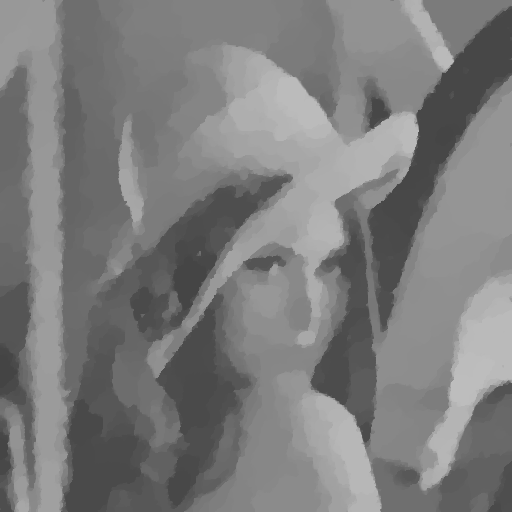
\includegraphics[width=\textwidth]{img/approximation/rof/rof_start/001lena.png}
                    \caption{$\lambda = 0.01$}
                \end{subfigure}
                \caption[First estimate of $\lambda$ for the ROF model.]{Approximation of the Lena image with the ROF model. The higher $\lambda$ the closer the approximation to the original image.}
            \label{fig:rof_lena_first_compare}
            \end{figure}

            It seems not to be appropriable to go one one-thousandth steps and we already learned, that a small parameter does not lead to the desired results. We turn our interest to the other extrem setting. We use the range from $0.1$ to $1$ in one-tenth steps. It not only leads to the perfect fit, it also produces good approximations $u$ of our input image $g$. This can be seen in figure \ref{fig:rof_lena_second_compare} and the estimated values in table \ref{tab:best_fit_compare}.

            \begin{figure}[!ht]
                \centering
                \begin{subfigure}[b]{0.18\textwidth}
                    \includegraphics[width=\textwidth]{img/approximation/rof/rof_start/01lena.png}
                    \caption{$\lambda = 0.1$}
                \end{subfigure}
                \begin{subfigure}[b]{0.18\textwidth}
                    \includegraphics[width=\textwidth]{img/approximation/rof/rof_start/02lena.png}
                    \caption{$\lambda = 0.2$}
                \end{subfigure}
                \begin{subfigure}[b]{0.18\textwidth}
                    \includegraphics[width=\textwidth]{img/approximation/rof/rof_start/03lena.png}
                    \caption{$\lambda = 0.3$}
                \end{subfigure}
                \begin{subfigure}[b]{0.18\textwidth}
                    \includegraphics[width=\textwidth]{img/approximation/rof/rof_start/04lena.png}
                    \caption{$\lambda = 0.4$}
                \end{subfigure}
                \begin{subfigure}[b]{0.18\textwidth}
                    \includegraphics[width=\textwidth]{img/approximation/rof/rof_start/05lena.png}
                    \caption{$\lambda = 0.5$}
                \end{subfigure}
                \begin{subfigure}[b]{0.18\textwidth}
                    \includegraphics[width=\textwidth]{img/approximation/rof/rof_start/06lena.png}
                    \caption{$\lambda = 0.6$}
                \end{subfigure}
                \begin{subfigure}[b]{0.18\textwidth}
                    \includegraphics[width=\textwidth]{img/approximation/rof/rof_start/07lena.png}
                    \caption{$\lambda = 0.7$}
                \end{subfigure}
                \begin{subfigure}[b]{0.18\textwidth}
                    \includegraphics[width=\textwidth]{img/approximation/rof/rof_start/08lena.png}
                    \caption{$\lambda = 0.8$}
                \end{subfigure}
                \begin{subfigure}[b]{0.18\textwidth}
                    \includegraphics[width=\textwidth]{img/approximation/rof/rof_start/09lena.png}
                    \caption{$\lambda = 0.9$}
                \end{subfigure}
                \begin{subfigure}[b]{0.18\textwidth}
                    \includegraphics[width=\textwidth]{img/approximation/rof/rof_start/1lena.png}
                    \caption{$\lambda = 1$}
                \end{subfigure}
                \caption[Second estimate of $\lambda$ for the ROF model.]{Approximation of the Lena image with the ROF Model. Again, the higher $\lambda$ the closer the approximation to the original image.}
            \label{fig:rof_lena_second_compare}
            \end{figure}

            We only consider approximations $u$, which have a PSNR less than 40, compared to the input image $g$. Then there are only the choices $0.1$, $0.2$ and $0.3$. Because the PSNR for $\lambda = 0.3$ is at 39, we also dropped this value. As the energy in the case $\lambda = 0.1$ is significantly smaller as for $\lambda = 0.2$, we choose $\lambda = 0.1$ as our best estimate.

            \begin{table}[!ht]
                \centering
                \begin{tabular}{| l | l | l | l | l | l |}
                \hline
                $\lambda$ & MSE & PSNR & Energy \\ \hline\hline
                0.1 & 23 & 34 & 1,384,210 \\ \hline
                0.2 & 12 & 38 & 1,595,940 \\ \hline
                0.3 & 8 & 39 & 1,717,590 \\ \hline
                0.4 & 6 & 41 & 1,802,040 \\ \hline
                0.5 & 4 & 42 & 1,865,850 \\ \hline
                0.6 & 3 & 43 & 1,916,280 \\ \hline
                0.7 & 3 & 44 & 1,957,350 \\ \hline
                0.8 & 2 & 44 & 1,991,410 \\ \hline
                0.9 & 2 & 45 & 2,020,130 \\ \hline
                1.0 & 2 & 46 & 2,044,670 \\ \hline
                \end{tabular}
                \caption[Overview of values for $\lambda$ for the ROF model.]{The estimates for all $\lambda$ in $\{0.1, 0.2, ..., 1.0\}$.}
                \label{tab:best_fit_compare}
            \end{table}

        To the end of this subsection let us mention that we did not discretize the domain $\Omega$ in this framework. For this, we observe other values for $\lambda$ as proposed in \cite{Chambolle10afirst-order}.

        \subsection{Estimation of $\tau$}
        \label{sub:estimation_of_tau_rof}

            We find, that for $\lambda = 0.1$ the best choice for the time-step is $\tau = 0.63$. This value rises by running tests for $\tau$ starting at $0.01$ and increasing it by $0.01$ until we reach $0.99$. For this test procedure we make use of three different images: Lena (grayscaled) Hepburn (RGB) and Van Gogh (RGB). As table \ref{tab:best_tau_compare} reveals, the suggested value for $\tau$ is always under the first ten estimates, where the table was sorted by the number of iterations and the run-time of the algorithm. We also learn from this table, that the time-step $\tau$ couples with the input image. This means, that $\tau = 0.63$ is a good guess and likely to yield a fast convergence, but does not hold for each and every image. This coupling is not only between the input image $g$ and $\tau$, we further find it between $\lambda$ and $\tau$. One example, how this coupling influences the algorithm is, If we let $\lambda = 0.01$ and using $\tau = 0.63$ we observe 1110 iterations in the primal-dual algorithm. If we compare this with 240 iterations for $\lambda = 0.1$ (table \ref{tab:best_tau_compare}), we see that this coupling has a big influence on finding valid estimates for $\lambda$ and $\tau$ beforehand.

            \begin{table}[!ht]
                \centering
                \begin{tabular}{| l | l | l | l | l | l | l | l | l | l |}
                    \hline
                    \multicolumn{4}{|c|}{Lena Image} & \multicolumn{3}{|c|}{Hepburn Image} & \multicolumn{3}{|c|}{Van Gogh Image} \\ \hline\hline
                    No. & $\tau$ & Iter & Run-Time & $\tau$ & Iter & Run-Time & $\tau$ & Iter & Run-Time \\ \hline
                    1 & 0.63 & 100 & 0.84 & 0.65 & 130 & 2.75 & 0.63 & 90 & 0.87 \\ \hline
                    2 & 0.74 & 120 & 1.03 & 0.9 & 150 & 3.13 & 0.68 & 110 & 1.07 \\ \hline
                    3 & 0.86 & 120 & 1.09 & 0.85 & 160 & 3.35 & 0.76 & 120 & 1.14 \\ \hline
                    4 & 0.94 & 140 & 1.11 & 0.78 & 200 & 4.23 & 0.86 & 140 & 1.36 \\ \hline
                    \vdots &  &  &  &  &  &  &  &  &  \\ \hline
                    10 & 0.63 & 240 & 2.16 & 0.63 & 260 & 5.42 & 0.78 & 190 & 1.72 \\ \hline
                \end{tabular}
                \caption[Best estimate of $\tau$ for the ROF model.]{Setting $\tau = 0.63$ provides a good guess for fast convergence.}
                \label{tab:best_tau_compare}
            \end{table}

            Knowing nothing about the best time-step $\tau$ by initialization of the algorithm, makes the proposed approach a bit incosistent. The coupling makes it not easy to determine the best parameter for $\tau$. This problem is still ongoing research. Nonetheless, having a stable framework like this, to minimize the energy for the ROF model, is a great approach and yields good approximations $u$ of the input images $g$, as figure \ref{fig:best_rof_hepburn} shows for the Audrey Hepburn image.

            \begin{figure}[!ht]
                \centering
                \begin{subfigure}[b]{0.32\textwidth}
                    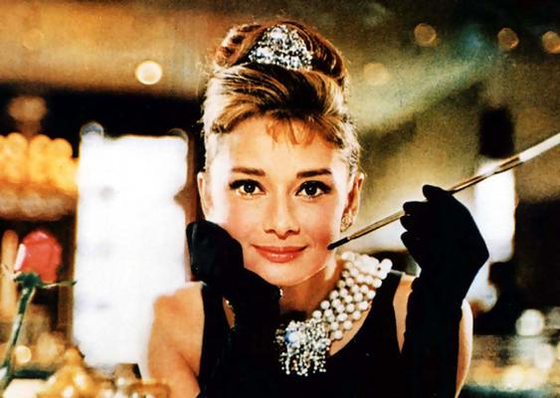
\includegraphics[width=\textwidth]{img/hepburn.png}
                    \caption{The original image of Audrey Hepburn.}
                \end{subfigure}
                \begin{subfigure}[b]{0.32\textwidth}
                    \includegraphics[width=\textwidth]{img/best_rof_hepburn.png}
                    \caption{Approximation using the proposed parameter.}
                \end{subfigure}
                \begin{subfigure}[b]{0.32\textwidth}
                    \includegraphics[width=\textwidth]{img/better_rof_hepburn.png}
                    \caption{Approximation using $\lambda = 0.01$.}
                \end{subfigure}
                \caption[Best approximation using the ROF model with Hepburn image.]{Approximation of the Audrey Hepburn image with the ROF model. In (b) we set $\lambda = 0.1, \tau = 0.63$, where (c) resembles $\lambda = 0.01, \tau = 0.63$.}
                \label{fig:best_rof_hepburn}
            \end{figure}

            Overall, we suggest for the primal-dual algorithm the setting $\theta = 1$, $\lambda = 0.1$ and $\tau = 0.63$, for which we derive the approximation $u$ of $g$ in a reasonable run-time and visibly good results.

    \section{Image Approximation using the TVL1 Model} % (fold)
    \label{sec:image_approximation_using_the_tvl1_model}

        We now turn our focus on the TVL1 model. As this model has a fast CPU version, we also do not provide a parallelized version for a GPU. Additionally, we can adapt a lot of operations from the previous section. The gradient operators and computation of the proximity operator for $F^{\ast}(p) = \delta_{P}(p)$ remain completely the same. The primal-dual algorithm with the extrapolation step is consistent and can be used. The only difference to the ROF model, is the computation of $(\textnormal{Id} + \tau\,\partial\,G)^{-1}(\tilde{u})$ and we need to change the function for our stopping criterion. In equation \ref{eq:prox_g_tvl1} we showed, that this proximity operator is of the form

            $$
                u = (\textnormal{Id} + \tau\,\partial\,G)^{-1}(\tilde{u}) \Longleftrightarrow u_{i, j} = 
                    \begin{dcases*}
                        \tilde{u}_{i,j} - \tau\lambda & \textnormal{if\, $\tilde{u}_{i,j} - g_{i,j} > \tau\lambda$,} \\
                        \tilde{u}_{i,j} + \tau\lambda & \textnormal{if\, $\tilde{u}_{i,j} - g_{i,j} < - \tau\lambda$,} \\
                        g_{i, j} & \textnormal{if\, $|\tilde{u}_{i,j} - g_{i,j}| \le \tau\lambda$}.
                    \end{dcases*}
            $$
        This means, that our update on the variable $u$ or more precisely $u^{n+1}_{i,j,k}$, depends on the current estimate $\tilde{u}$ and the input image $g$. To save run-time, we pre-compute
            $$
                fac = tau*lambda \,\,\, \textnormal{and} \,\,\, est = u^{n}_{i,j,k} - g_{i,j,k}.
            $$
        Since, these values need to be computed in each if-statement, we calculate it once - before the if-statements occur - and make use of the values:
            $$
                u^{n+1}_{i,j,k} = 
                    \begin{dcases*}
                        u^{n}_{i,j,k} - fac & \textnormal{if\, $est > fac$,} \\
                        u^{n}_{i,j,k} + fac & \textnormal{if\, $est < - fac$,} \\
                        g_{i,j,k} & \textnormal{if\, $abs(est) \le fac$}.
                    \end{dcases*}
            $$

        Now, the only thing we need to change in in algorithm \ref{alg:primal_descent} is the last line of code in the inner for-loop. In this line we compute the proximity operator, so we fit the code to the TVL1 model and obtain:

            \begin{algorithm}[Primal Descent]
                \begin{lstlisting}
template<typename T>
void primal_desc(T* p_x, T* p_y, T* u, T* g, T tau, T lambda, int M, int N, int C) {
  T dx, dy, sum;
  int index;
  for (int k = 0; k < C; k++) {
    for (int i = 0; i < N; i++) {
      for (int j = 0; j < M; j++) {
        index = j + i * M + k * N * M;
        dx = (i+1<N ? p_x[index] : 0.f) -
             (i>0 ? p_x[j + (i-1) * M + k * N * M] : 0.f);
        dy = (j+1<M ? p_y[index] : 0.f) -
             (i>0 ? p_y[(j-1) + i * M + k * N * M] : 0.f);
        sum = tau * (dx + dy);
        sum += u[index];
        fac = tau*lambda;
        est = sum - g[i];
        if (est > fac) u[i] = sum - fac;
        if (est < -fac) u[i] = sum + fac;
        if (abs(est) <= fac) u[i] = g[i];
      }
    }
  }
}
                \end{lstlisting}
                where the template value $T$ is mostly set as float.
            \end{algorithm}

            Because, we changed the $L^{2}$ norm in the data fidelity term of the ROF functional to the $L^{1}$ norm, we need to take this into account in the stopping criterion. We only need to substitute the line of code, where the data fidelity term enters the computation of the energy itself. According to the C++-function in \ref{alg:stop_rof_tvl1}, we only change the last line of code in the inner for-loops, from
                $$
                    energy += (lambda/2 * pow(u[X] - g[X], 2)) \,\,\, \textnormal{to} \,\,\, energy += (lambda * (abs(u[X] - g[X]))).
                $$

            These substitutions are all it takes and we are completely set up with the TVL1 model. It is now left to provide good estimates for the input values $\lambda$ and $\tau$. We set again $\theta = 1$ and allocate $u, \bar{u}, g \in [0, 255]^{C}$, where $C$ is the number of color channels.

            \subsection{Estimation of $\lambda$} % (fold)
            \label{sub:estimation_of_lambda_tvl1}

                For the TVL1 model, estimating a good $\lambda$ was an easy task compared to the ROF model. The reason for this is, that in \cite{Chambolle10afirst-order} they proposed this model without the scaling factor $h^{2}$, like we do in this work. They already suggested to set $\lambda = 0.7$. We adapted this idea and tested all values from $0.1$ to $1$ by increasing $\lambda$ for each approximation by $0.1$. This evolution process is shown in figure \ref{fig:tvl1_lena_first_compare}.
                
                \begin{figure}[!ht]
                \centering
                \begin{subfigure}[b]{0.18\textwidth}
                    \includegraphics[width=\textwidth]{img/approximation/tvl1/01lena.png}
                    \caption{$\lambda = 0.1$}
                \end{subfigure}
                \begin{subfigure}[b]{0.18\textwidth}
                    \includegraphics[width=\textwidth]{img/approximation/tvl1/02lena.png}
                    \caption{$\lambda = 0.2$}
                \end{subfigure}
                \begin{subfigure}[b]{0.18\textwidth}
                    \includegraphics[width=\textwidth]{img/approximation/tvl1/03lena.png}
                    \caption{$\lambda = 0.3$}
                \end{subfigure}
                \begin{subfigure}[b]{0.18\textwidth}
                    \includegraphics[width=\textwidth]{img/approximation/tvl1/04lena.png}
                    \caption{$\lambda = 0.4$}
                \end{subfigure}
                \begin{subfigure}[b]{0.18\textwidth}
                    \includegraphics[width=\textwidth]{img/approximation/tvl1/05lena.png}
                    \caption{$\lambda = 0.5$}
                \end{subfigure}
                \begin{subfigure}[b]{0.18\textwidth}
                    \includegraphics[width=\textwidth]{img/approximation/tvl1/06lena.png}
                    \caption{$\lambda = 0.6$}
                \end{subfigure}
                \begin{subfigure}[b]{0.18\textwidth}
                    \includegraphics[width=\textwidth]{img/approximation/tvl1/07lena.png}
                    \caption{$\lambda = 0.7$}
                \end{subfigure}
                \begin{subfigure}[b]{0.18\textwidth}
                    \includegraphics[width=\textwidth]{img/approximation/tvl1/08lena.png}
                    \caption{$\lambda = 0.8$}
                \end{subfigure}
                \begin{subfigure}[b]{0.18\textwidth}
                    \includegraphics[width=\textwidth]{img/approximation/rof/rof_start/09lena.png}
                    \caption{$\lambda = 0.9$}
                \end{subfigure}
                \begin{subfigure}[b]{0.18\textwidth}
                    \includegraphics[width=\textwidth]{img/approximation/rof/rof_start/1lena.png}
                    \caption{$\lambda = 1$}
                \end{subfigure}
                \caption[Best estimate of $\lambda$ for the TVL1 model.]{Approximation of the Lena image with the TVL1 Model.}
            \label{fig:tvl1_lena_first_compare}
            \end{figure}

            As one can see, the value $\lambda = 0.7$ yields reasonable results with less noise, no over-smoothing and sharp edges. The values $0.6$ and $0.8$ would also fit, but we decided to follow Pock and Chambolle (\cite{Chambolle10afirst-order}) with their suggestion.

            % subsection best_ (end)

            \subsection{Estimation of $\tau$} % (fold)
            \label{sub:estimation_of_tau_tvl1}
                
                We apply the same procedure to estimate the best time-step parameter $\tau$ as in subsection \ref{sub:estimation_of_tau_rof}. We use again the images Lena, Hepburn and Van Gogh for the evaluation. There is only one parameter, which appeares under the sixth fastest convergence rates: $\tau = 0.97$, c.f. table \ref{tab:best_tau_compare_tvl1}. For this we suggest to set $\tau = 0.97$. Unfortunatelly, we have again a coupling of the image, $\lambda$ and $\tau$. This means, that using the estimate $\tau = 0.97$ does not guarantee fast convergence with every image.

                \begin{table}[!ht]
                    \parbox{\linewidth}{
                    \centering
                        \begin{tabular}{| l | l | l | l | l | l | l |}
                            \hline
                            & \multicolumn{2}{|c|}{Lena Image} & \multicolumn{2}{|c|}{Hepburn Image} & \multicolumn{2}{|c|}{Van Gogh Image} \\ \hline\hline
                            $\tau$ & Iter & Run-Time & Iter & Run-Time & Iter & Run-Time \\ \hline
                            0.97 & 370 & 3.44 & 580 & 12.66 & 1500 & 15.47 \\ \hline
                        \end{tabular}
                    }
                    \caption[Best estimate of $\tau$ for the TVL1 model.]{The results for the best estimate $\tau = 0.97$.}
                    \label{tab:best_tau_compare_tvl1}
                \end{table}

                In figure \ref{fig:best_tvl1_landscape} we show the result for our suggested framework by setting $\theta = 1, \lambda = 0.7$ and $\tau = 0.97$ using the Landscape image. The underlying image is color valued and it only took $530$ iterations until convergence. In run-time it took about $4.4$ seconds and is for that quite fast. Even though, the TVL1 model yields good approximations, we clearly see, that it is not able to preserve edges well enough. Some contours vanish and we see some over-smoothing in the image itself. If we set $\lambda = 1.2$, we observe much better results, since the higher parameter for $\lambda$ assures, that the approximation is closer to the input image $g$. With this $\lambda$ and again $\tau = 0.97$, we observe $850$ iteration steps in the primal-dual algorithm. Again, the coupling of $\lambda$, $\tau$ and the image $g$ does not ensure a fast convergence.

                \begin{figure}[!ht]
                    \centering
                    \begin{subfigure}[b]{0.32\textwidth}
                        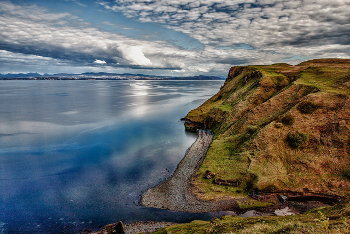
\includegraphics[width=\textwidth]{img/landscape.png}
                        \caption{The original Landscape image.}
                    \end{subfigure}
                    \begin{subfigure}[b]{0.32\textwidth}
                        \includegraphics[width=\textwidth]{img/best_tvl1_landscape.png}
                        \caption{Approximation using the proposed parameter.}
                    \end{subfigure}
                    \begin{subfigure}[b]{0.32\textwidth}
                        \includegraphics[width=\textwidth]{img/better_tvl1_landscape.png}
                        \caption{Approximation using $\lambda = 1.2$.}
                    \end{subfigure}
                    \caption[Best approximation using the TVL1 model with Landscape image.]{Approximation of the Landscape image with the TVL1 model.}
                    \label{fig:best_tvl1_landscape}
                \end{figure}

                The TVL1 model yields good approximations $u$ and as we will see is able to remove Gaussian and salt and pepper noise from images. But, we are also interested in preserving edges in the approximations. For that, the convex relaxed Mumford-Shah model, as seen in section \ref{sec:the_convex_relaxed_mumford_shah_model}, is therefore the right choice.

            % subsection best_tau_estimation (end)
        
    % section image_approximation_using_the_tvl1_model (end)

    \section{Image Approximation using the Real-Time Minimizer} % (fold)
    \label{sec:image_approximation_using_the_real_time_minimizer}
        
        In the case of the real-time minimizer for the Mumford-Shah model, which only has real-time applicability on a GPU, we can again adapt most of the code from the ROF model. Even though, it runs in real-time, we were more interested in the framework itself. For that, we only provide a CPU implementation, which also has a good performance.

        The function $G$ is almost the same as in the ROF model, except the scaling parameter $\frac{\lambda}{2}$. But for that, we only need to exchange one line of code. The line
            $$
                u[index] = (sum + tau * lambda * g[index]) / (1.f + tau * lambda);
            $$
        becomes
            $$
                u[index] = (sum + 2 * tau * g[index]) / (1.f + 2 * tau);.
            $$
        Everything else in algorithm \ref{alg:primal_descent} remains the same. In algorithm \ref{alg:dual_ascent} we need to exchange two lines of code, where we take into account that the proximity operator for $R_{MS}^{\ast}(\tilde{p})$ is computed by
            $$
                p = \left( \textnormal{Id} + \sigma \partial R_{MS}^{\ast} \right)^{-1}(\tilde{p}) \Longleftrightarrow p_{i,j} =
                    \begin{dcases*}
                        \frac{\lambda}{\lambda + \sigma} \tilde{p}, & \textnormal{if $|\tilde{p}| \le \sqrt{\frac{\nu}{\lambda}\sigma(\sigma + 2\lambda)}$,} \\
                        0 & \textnormal{else.}
                    \end{dcases*}
            $$
        For the implementation we make use of the run-time saving method to pre-compute some values and use them afterwards in each calculation. We set $fac = (2 * lambda) / (sigma + 2 * lambda)$, $p_{abs} = |p^{n}_{i,j,k}| = sqrt(dx*dx+dy*dy)$ and compute the bound by $B = sqrt((nu / lambda) * sigma * (sigma + 2 * lambda))$. Then we rewrite the proximity operator to
            $$
                p^{n+1}_{i,j,k} =
                    \begin{dcases*}
                        fac*p^{n}_{i,j,k} & \textnormal{if $p_{abs} \le B$,} \\
                        0 & \textnormal{else.}
                    \end{dcases*}
            $$
        We change the computations, in which we compute $p^{n+1}_{x}$ and $p^{n+1}_{y}$, with respect to the proximity operator of $R_{MS}^{\ast}(\tilde{p}^{n})$.

            \begin{algorithm}[Dual Ascent]
                \begin{lstlisting}
template<typename T>
void dual_asc(T* p_x, T* p_y, T* u_bar, T sigma, T lambda, T nu, int M, int N, int C) {
  T dx, dy;
  int index;
  T fac = (2 * lambda) / (sigma + 2 * lambda);
  T B = sqrt((nu / lambda) * sigma * (sigma + 2 * lambda));
  for (int k = 0; k < C; k++) {
    for (int i = 0; i < N; i++) {
      for (int j = 0; j < M; j++) {
        index = j + i * M + k * N * M;
        dx = i+1<N ? u_bar[j + (i+1) * M + k * N * M]-u_bar[index] : 0;
        dy = j+1<M ? u_bar[(j+1) + i * M + k * N * M]-u_bar[index] : 0;
        dx = p_x[index] + sigma * dx;
        dy = p_y[index] + sigma * dy;
        p_abs = sqrt(dx*dx+dy*dy);
        p_x[index] = p_abs <= B ? fac * dx : 0;
        p_y[index] = p_abs <= B ? fac * dy : 0;
      }
    }
  }
}
                \end{lstlisting}
                where the template value $T$ is mostly set as float.
            \end{algorithm}

        The function to determine convergence, needs to be rewritten. Using the proposed method in equation \ref{eq:stop_realtime_model} we compute after each iteration step of the primal-dual algorithm
            $$
                ||u^{n+1} - u^{n}|| \le \varepsilon,
            $$
        with $\varepsilon = 5 \cdot 10^{-5}$ and with the definition of the underlying norm
            $$
                ||u^{n+1} - u^{n}|| = \frac{1}{N \cdot M} \sum_{k = 1}^{C} \sum_{i = 1}^{N} \sum_{j = 1}^{M} |u_{i,j,k}^{n+1} - u_{i,j,k}^{n}|.
            $$
        As in the extrapolation function, we can compute the norm within one for loop for letting $u^{n}, u^{n+1} \in \mathbb{R}^{N \cdot M \cdot C}$. Overall, we summarize this in the following function:

            \begin{algorithm}[Stopping Criterion]
                    \label{alg:stop_realtime}
                        \begin{lstlisting}
template<typename T>
T Stop(T* u, T* u_n, int M, int N, int C) {
  T energy = 0.f;
    for (int i = 0; i < N*M*C; i++) {
      energy += abs(u[i] - u_n[i]);
    }
  return (energy/(N*M));
}
                    \end{lstlisting}
                    where the template value $T$ is mostly set as float.
                \end{algorithm}

        As we used the second algorithm of section \ref{sec:a_firs_order_primal_dual_algorithm}, namely algorithm \ref{alg:realtime_primal_dual_algorithm}, we additionally propose this version in C++ code:

        \begin{algorithm}[Primal-Dual Algorithm]
        \label{alg:primal_dual_2}
            \begin{lstlisting}
template<typename T>
void RealTimeMinimizer(T* u, T* g, T lambda, T nu, int M, int N, int C, int iter) {
  T tau = 1.f / 4.f;
  T sigma = 1.f / 2.f;
  T theta = 2.f;
  T* u_bar = new T[M*N*C];
  T* u_prev = new T[M*N*C];
  T* p_x = new T[M*N*C];
  T* p_y = new T[M*N*C];

  for (int k = 1; k <= iter; k++) {
    void dual_asc(p_x, p_y, u_bar, sigma, lambda, nu, M, N, C);
    void primal_desc(p_x, p_y, u, g, tau, M, N, C);
    theta = (T)1 / sqrt(1 + 4 * tau); tau *= theta; sigma /= theta;
    void extrapolation(u_bar, u, u_prev, theta, M, N, C);
    if (k%10 == 0) {
      stop = h * ;
      if (Stop(u, u_n, M, N, C) <= 5 * 1E-5) {
        break;
      }
    }
  }

  delete [] u_bar;
  delete [] u_prev;
  delete [] p_x;
  delete [] p_y;
}
            \end{lstlisting}
            where the template value $T$ is mostly set as float.
        \end{algorithm}

        The difference in this framework is, that the primal-dual function does not take the parameter $\tau$ as an argument, since algorithm \ref{alg:realtime_primal_dual_algorithm} suggests, that this value is fixed by initialization. Instead the function takes the second parameter of the corresponding model, namely $\nu$. Additionally, we compute the updates on $\theta, \tau$ and $\sigma$ in each iteration step of the primal-dual algorithm. It is left to present the estimation for the parameters $\lambda$ and $\nu$. For this particular framework we followed Strekalovskiy and Cremers in \cite{Strekalovskiy-Cremers-eccv14} and set $u, \bar{u}, g \in [0,1]^{C}$, where $C$ is again the number of color channels.

        \subsection{Best $\lambda$ and $\nu$ estimation} % (fold)
        \label{sub:best_parameter_estimation_rt}
            
            For this model we have two parameters, which can be combined in a lot of ways. Finding parameters $\lambda$ and $\nu$ take several estimation steps. We will not provide the whole procedure of this process, since it could fill a huge amount of pages. But, we discuss our estimation in a short term and the corresponding results.

            Initially we set $\nu = 0.1$ and seek for $\lambda$ using the Audrey Hepburn image. For the piecewise-constant model, we try several possible $\lambda$ in between $100$ and $1000$. It turns out, that there are no big changes if $\lambda \ge 500$ and so we use the setting $\lambda = 500$. In the piecewise-smooth model, we start with the guess $\lambda = 0.1$, which is too small. By testing each $\lambda$ by an increased value of $0.1$, we find, that at about $1.8$ to $2.2$, there is a good chance for a good fit. Of course, testing then the value $\nu$, has also an influence on $\lambda$ again. Nonetheless, we fix $\lambda = 2$ and test for $\nu$. For the piecewise-smooth case, we start with $0.1$ to $1$ in 0.1-steps. We focus on the PSNR value. We assume that it should be over $30$, but not too close to $40$. A good fit for this setting is $\nu = 0.2$. In figure \ref{fig:realtime_hepburn_compare}, we see, that this setting indeed yields a good smooth approximations $u$. Learning that $\nu$ lies in the range of $0.1$ to $1$, we adapt the value for $\nu$ for the piecewise-constant model. Unfortunately, it turns out, that this setting needs a higher value for $\nu$, to be able to cope with the increased value for $\lambda$ in the minimum function of $R_{MS}$. Testing again each $\nu$ in the range of $0.1$ to $1$ by increasing it by $0.1$ in each estimate, we find that $\nu = 0.7$ is a good choice. See again figure \ref{fig:realtime_hepburn_compare} for this setting.

            \begin{table}[!ht]
                \centering
                \begin{tabular}{| l | l | l | l | l |}
                \hline
                $\lambda$ & $\nu$ & Iterations & Run-Time & PSNR \\ \hline\hline
                2 & 0.2 & 80 & 1.37 & 32 \\ \hline
                500 & 0.7 & 430 & 7.2 & 23 \\ \hline
                \end{tabular}
                \caption[Comparison of $\lambda$ and $\nu$ in the Mumford-Shah real-time framework.]{Best estimates in the piecewise-constant and piecewise-smooth case.}
                \label{tab:best_parameters_rt}
            \end{table}

            The corresponding images to the proposed values for $\lambda$ and $\nu$ can be seen in figure \ref{fig:realtime_hepburn_compare}. The estimated values for the PSNR, number of iterations, run-time and the parameters suggested, can be found in table \ref{tab:best_parameters_rt}.

            \begin{figure}[!ht]
                \centering
                \begin{subfigure}[b]{0.32\textwidth}
                    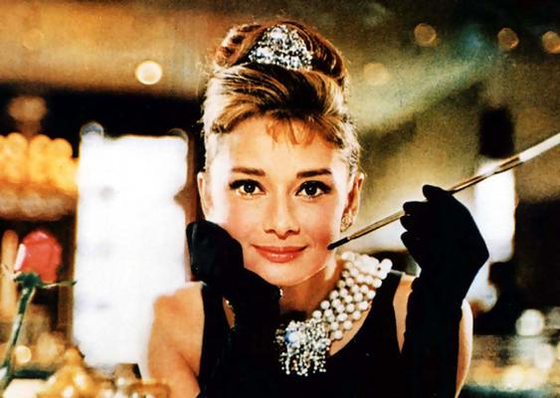
\includegraphics[width=\textwidth]{img/hepburn.png}
                    \caption{Original image.}
                \end{subfigure}
                \begin{subfigure}[b]{0.32\textwidth}
                    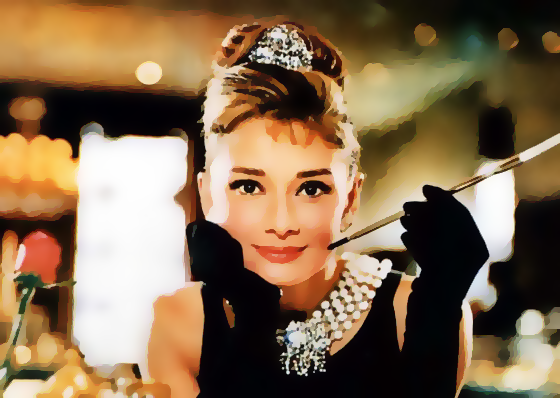
\includegraphics[width=\textwidth]{img/best_pws_hepburn.png}
                    \caption{$\alpha = 2, \lambda = 0.2$}
                \end{subfigure}
                \begin{subfigure}[b]{0.32\textwidth}
                    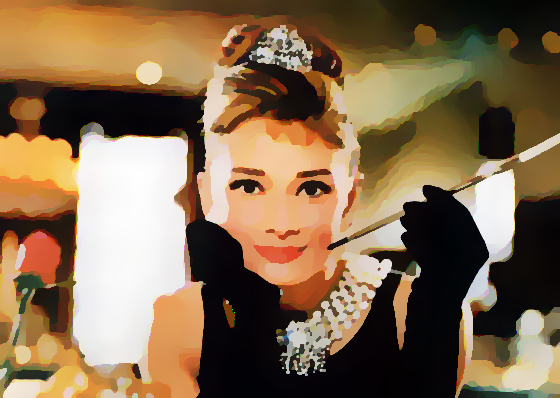
\includegraphics[width=\textwidth]{img/best_pwc_hepburn.png}
                    \caption{$\alpha = 500, \lambda = 0.7$}
                \end{subfigure}
                \caption[Comparing Audrey Hepburn pwc. and pws. using Mumford-Shah.]{Approximation of the Audrey Hepburn image with the piecewise-smooth and piecewise-constant Mumford-Shah model.}
            \label{fig:realtime_hepburn_compare}
            \end{figure}

            Further, there is no need to find a good estimate of the time-step $\tau$, because this value is updated in each iteration seperately and is coupled with the parameter $\theta$. As suggested in algorithm \ref{alg:primal_dual_2} we pre-computed it with $\tau = \frac{1}{2d}$, where $d = 2$, since the dimension of $\Omega$ is two.\\

        % subsection best_parameter_estimation_rt (end)

    % section approximation_using_the_real_time_minimizer (end)

    Now, that we are set up with the pure image approximation and the corresponding implementation issues, let us turn our focus on applications to imaging. We start with one application of the real-time minimizer of the Mumford-Shah functional, namely image cartooning.

    \section{Image Cartooning} % (fold)
    \label{sec:image_cartooning}
        
        In this section we present a technique to turn an input image $g$ into a cartooned image $u$. For this we will make use of the real-time minimizer for the Mumford-Shah functional, presented in section \ref{sec:the_mumford_shah_model}. We further introduce a concept to highlight the edges in the cartooned images, first proposed in \cite{Strekalovskiy-Cremers-eccv14}. For this we make explicit use of the set $K_{MS}$, as modeled in equation \ref{eq:edge_set_k}. We then present cartooned images - piecewise-constant approximations - with edge highlighting.

        % subsection another_data_fidelity_term (end)

        \subsection{Edge Highlighting} % (fold)
        \label{sub:edge_highlighting}
            
            The idea, proposed by Strekalovskiy and Cremers in \cite{Strekalovskiy-Cremers-eccv14}, is to use the edge set $K_{MS}$ in order to highlight edges in the approximation $u$.

            For that, assume that $(i,j) \in K_{MS}$ then we have $|(\nabla u)_{i,j}| \ge \sqrt{\frac{\nu}{\lambda}}$ by definition. This notation is equivalent to
                $$
                    \frac{|(\nabla u)_{i,j}|}{\sqrt{\frac{\nu}{\lambda}}} \ge 1.
                $$
            Further, we compute $|(\nabla u)_{i,j}| \le \sqrt{4} = 2$. This equation holds with the definition for $\nabla$, c.f. definition \ref{def:discrete_gradient_operator}, since
                \begin{eqnarray}
                    |(\nabla u)_{i,j}| &=& \sqrt{(u_{i+1,j} - u_{i,j})^{2} + (u_{i,j+1} - u_{i,j})^{2}} \notag \\
                    &=& \sqrt{u_{i+1,j}^{2} - 2u_{i+1,j}u_{i,j} + u_{i,j}^{2} + u_{i,j+1}^{2} - 2u_{i,j+1}u_{i,j} + u_{i,j}^{2}} \notag \\
                    &=& \sqrt{2u_{i,j}^{2} + u_{i+1,j}^{2} + u_{i,j+1}^{2} - 2u_{i,j}\left(u_{i+1,j} - u_{i,j+1}\right)} \notag \\
                    &\overbrace{\le}^{u \in [0,1]}& \sqrt{2 + 1 + 1} = \sqrt{4} = 2.
                \end{eqnarray}
            And for that
                $$
                    1 \le \frac{|(\nabla u)_{i,j}|}{\sqrt{\frac{\nu}{\lambda}}} \le \frac{2}{\sqrt{\frac{\nu}{\lambda}}}.
                $$
            Applying the logarithm function to each of the terms we get
                $$
                    0 \le \log \left( \frac{|(\nabla u)_{i,j}|}{\sqrt{\frac{\nu}{\lambda}}} \right) \le \log \left( \frac{2}{\sqrt{\frac{\nu}{\lambda}}} \right).
                $$
            If we now divide each term by the one on the rightmost, we observe
                $$
                    0 \le \frac{\log \left( \frac{|(\nabla u)_{i,j}|}{\sqrt{\frac{\nu}{\lambda}}} \right)}{\log \left( \frac{2}{\sqrt{\frac{\nu}{\lambda}}} \right)} \le 1.
                $$
            With these calculations, we now define a $v \in [0, 1]$ by
                $$
                    v := \frac{\log \left( \frac{|(\nabla u)_{i,j}|}{\sqrt{\frac{\nu}{\lambda}}} \right)}{\log \left( \frac{2}{\sqrt{\frac{\nu}{\lambda}}} \right)},
                $$
            then, since $\nu$ and $\lambda$ are constant values, this parameter $v$ only increases if $|(\nabla u)_{i,j}|$ increases and decreases if $|(\nabla u)_{i,j}|$ decreases, because $\sqrt{\frac{\nu}{\lambda}}$ is a constant factor and the logarithm function is monotonically increasing. The value $v$ serves as an edge indicator. The idea is then to multiply each pixel value $u$ by
                $$
                    1 - v \in [0, 1],
                $$
            if $(i, j) \in K_{MS}$. On the other hand, if $(i, j) \notin K_{MS}$ the value $u$ will not be changed. Then points in the image domain $\Omega$ with strong edges are painted darker.

            We implemented this technique of edge highlighting in our framework and tested it against the pure piecewise-constant approximation. Using the proposed values $\lambda = 500$ and $\nu = 0.7$, as suggested in section \ref{sub:best_parameter_estimation_rt}, we visiually compared an approximation with and without edge highlighting.

            \begin{figure}[!ht]
                \centering
                \begin{subfigure}[b]{0.32\textwidth}
                    \includegraphics[width=\textwidth]{img/hepburn.png}
                    \caption{Original image.}
                \end{subfigure}
                \begin{subfigure}[b]{0.32\textwidth}
                    \includegraphics[width=\textwidth]{img/best_pwc_hepburn.png}
                    \caption{Without edge highlighting.}
                \end{subfigure}
                \begin{subfigure}[b]{0.32\textwidth}
                    \includegraphics[width=\textwidth]{img/best_pwc_hepburn_eh.png}
                    \caption{With edge highlighting.}
                \end{subfigure}
                \caption[Cartooning example of Audrey Hepburn.]{Cartooning of the Hepburn image with $\lambda = 500$ and $\nu = 0.7$.}
            \label{fig:cartooning_hepburn_realtime}
            \end{figure}

        Figure \ref{fig:cartooning_hepburn_realtime} shows, that this technique clearly yields darker edges. Since, this highlighting takes place after applying the primal-dual algorithm, it does not slow down the code significantly. Summarizing this method in a C++-function, we have:

            \begin{algorithm}[Edge Highlighting]
                \begin{lstlisting}
template<typename T>
void edging(T* u, T lambda, T nu, int M, int N, int C) {
  for (int k = 0; k < C; k++) {
    for (int i = 0; i < N; i++) {
      for (int j = 0; j < M; j++) {
        int X = j + i * M + k * N * M;
        T dx = i + 1 < N ? u[j + (i+1) * M + k * N * M] - u[X] : 0;
        T dy = j + 1 < M ? u[j + 1 + i * M + k * N * M] - u[X] : 0;
        T norm = sqrt(dx*dx+dy*dy);
        T factor = sqrt(nu/lambda);
        if (norm >= factor) {
          T c = (T)1 / log(2/factor);
          u[X] = (1 - c * log(norm / factor)) * u[X];
        }
      }
    }
  }
}
                \end{lstlisting}
                where the template value $T$ is mostly set as float.
            \end{algorithm}

        % subsection edge_highlighting (end)

        In this section we showed, that the Mumford-Shah realtime minimizer is good in cartooning images and has the advantage of the discrete modeled set $K_{MS}$, which can be used for edge highlighting. But, the real-time framework has another application, namely denoising. We present this case together with the ROF and TVL1 model, respectively, in the next section.

    % section image_cartooning (end)

    \section{Image Denoising} % (fold)
    \label{sec:image_denoising}
        
        As discussed, an image $g$ consists of data and noise. Our goal is to remove the noise from an input image $g$ and get a smooth approximation $u$. We find different kinds of noise on images. The two most common are Gaussian and the so called salt and pepper noise. Where Gaussian noise is relatively easy to remove, salt and pepper noise is more robust, since it resembles extrem values on images. The ROF model and real-time minimizer for the Mumford-Shah model can handle Gaussian noise quite well, but are not able to remove salt and pepper noise accurately. However, the TVL1 model is able to manage both.

            \begin{figure}[!ht]
                \centering
                \begin{subfigure}[b]{0.24\textwidth}
                    \includegraphics[width=\textwidth]{img/images/lena.png}
                    \caption{Original image.}
                \end{subfigure}
                \begin{subfigure}[b]{0.24\textwidth}
                    \includegraphics[width=\textwidth]{img/images/lena_sp_noise.png}
                    \caption{25\% noise.}
                \end{subfigure}
                \begin{subfigure}[b]{0.24\textwidth}
                    \includegraphics[width=\textwidth]{img/denoising/salt_and_pepper_noise/rof/0007lena.png}
                    \caption{$\lambda = 0.007$}
                \end{subfigure}
                \begin{subfigure}[b]{0.24\textwidth}
                    \includegraphics[width=\textwidth]{img/denoising/salt_and_pepper_noise/rof/0008lena.png}
                    \caption{$\lambda = 0.008$}
                \end{subfigure}
                \caption[Salt and pepper denoising example: ROF.]{Salt and pepper denoising of the Lena image with the ROF Model.}
            \label{fig:denoising_lena_rof_sap}
            \end{figure}

        By evaluating a good $\lambda$ for both the ROF and TVL1 model, we tried our estimates of sections \ref{sec:image_approximation_using_the_rof_model} and \ref{sec:image_approximation_using_the_tvl1_model}. It turned out, that these $\lambda$ also fit perfectly to remove noise. The only thing we further tried to evaluate: finding a parameter $\lambda$ for the ROF model, so that it can remove salt and pepper noise. In fact, we found two values by testing all possible $\lambda$ in the range of $0.001$ to $1$ by increasing $\lambda$ in each test by $0.001$. Even though, the results $u$ are not as good as in the TVL1 model (see figure \ref{fig:denoising_lena_tvl1_sap}), the ROF model (figure \ref{fig:denoising_lena_rof_sap}) is able to remove this kind of noise in some sense, but as mentioned, not accurately. We also tested the real-time minimizer for the Mumford-Shah model, but could not find any pair of parameter, able to handle salt and pepper noise.

            \begin{figure}[!ht]
                \centering
                \begin{subfigure}[b]{0.31\textwidth}
                    \includegraphics[width=\textwidth]{img/images/lena.png}
                    \caption{Original image.}
                \end{subfigure}
                \begin{subfigure}[b]{0.31\textwidth}
                    \includegraphics[width=\textwidth]{img/images/lena_sp_noise.png}
                    \caption{25\% noise.}
                \end{subfigure}
                \begin{subfigure}[b]{0.31\textwidth}
                    \includegraphics[width=\textwidth]{img/denoising/salt_and_pepper_noise/tvl1/07lena.png}
                    \caption{$\lambda = 0.7$}
                \end{subfigure}
                \caption[Salt and pepper denoising example: TVL1.]{Salt and pepper denoising of the Lena image with the TVL1 Model.}
            \label{fig:denoising_lena_tvl1_sap}
            \end{figure}

        Comparing the denoising of images afflicted with Gaussian noise, we also compare the ROF model against the TVL1 model and the Mumford-Shah real-time model, figure \ref{fig:denoising_lena_gauss}.

            \begin{figure}[!ht]
                \centering
                \begin{subfigure}[b]{0.24\textwidth}
                    \includegraphics[width=\textwidth]{img/images/lena.png}
                    \caption{Original image}
                \end{subfigure}
                \begin{subfigure}[b]{0.24\textwidth}
                    \includegraphics[width=\textwidth]{img/images/lena_gauss_noise.png}
                    \caption{Noisy image}
                \end{subfigure}
                \begin{subfigure}[b]{0.24\textwidth}
                    \includegraphics[width=\textwidth]{img/denoising/gauss_noise/rof/002lena.png}
                    \caption{ROF: $\lambda = 0.02$}
                \end{subfigure}
                \begin{subfigure}[b]{0.24\textwidth}
                    \includegraphics[width=\textwidth]{img/denoising/gauss_noise/rof/003lena.png}
                    \caption{ROF: $\lambda = 0.03$}
                \end{subfigure}
                \begin{subfigure}[b]{0.24\textwidth}
                    \includegraphics[width=\textwidth]{img/denoising/gauss_noise/tvl1/06lena.png}
                    \caption{TVL1: $\lambda = 0.6$}
                \end{subfigure}
                \begin{subfigure}[b]{0.24\textwidth}
                    \includegraphics[width=\textwidth]{img/denoising/gauss_noise/tvl1/07lena.png}
                    \caption{TVL1: $\lambda = 0.7$}
                \end{subfigure}
                \begin{subfigure}[b]{0.24\textwidth}
                    \includegraphics[width=\textwidth]{img/denoising/gauss_noise/ms/207.png}
                    \caption{MS: $\lambda = 2, \nu = 0.7$}
                \end{subfigure}
                \begin{subfigure}[b]{0.24\textwidth}
                    \includegraphics[width=\textwidth]{img/denoising/gauss_noise/ms/205.png}
                    \caption{MS: $\lambda = 2, \nu = 0.5$}
                \end{subfigure}
                \caption[Removing Gaussian noise using the ROF, TVL1 and Mumford-Shah model.]{Removing Gaussian noise from the Lena image with the ROF, TVL1 and Mumford-Shah model.}
            \label{fig:denoising_lena_gauss}
            \end{figure}

        We see, that the Mumford-Shah model yields not the best approximations. From the evaluation of $\lambda$ and $\nu$, we already know, that we need $\lambda = 2$ for the piecewise-smooth approximation. By finding a suitable value $\nu$ it turns out, that the choice $\nu = 0.5$, as used in the piecewise-constant case, fits well. But also $\nu = 0.7$, as suggested for piecewise-smooth approximations, yields acceptable results. Even, if the noise is removed, the approximation is not comparable to those of the ROF and TVL1 model. These yield denoised approximations, which still preserve edges and areas accurately. In the last section, where we take a look at the convex relaxed Mumford-Shah model, we will see that this formulation is a good choice for removing Gaussian noise. The proposed real-time approach is not well suited for this class of problems.

        Further note, that denoising color valued images is also straightforward. We can apply the proposed methods channel-wise and then derive denoised approximations of, for instance, RGB images.

    % section image_denoising (end)

    \section{Image Inpainting} % (fold)
    \label{sec:image_inpainting}

        Image inpainting is the process to restore or fill lost image data. Images, which have a (huge) data loss, can be inpainted by using a model based on the ROF energy. In this section, we consider a modified version of the ROF model to derive a model for image inpainting. Let
            $$
                \mathcal{D} = \left\{ (i, j) \, | \, 1 \le i \le N, 1 \le j \le M \right\}
            $$
        denote the set of all discrete locations in our image domain. Since, we know that data is missing in the underlying image, we additionally define a set $\mathcal{I} \subseteq \mathcal{D}$, which holds all indices for which we have a data loss. The key idea is to take these two sets into account in the data fidelity term. We still use the total variaton as a regularizer, because we want to penalize jumps in the approximation $u$. But, we approximate $u$ only in terms of existing data. We have
            \begin{equation}
                \min_{u \in X} ||\nabla u||_{1} + \frac{\lambda}{2} \sum_{(i,j) \in \mathcal{D} \setminus \mathcal{I}} (u_{i,j} - g_{i,j})^{2}.
                \label{eq:inpainting_model}
            \end{equation}

        \begin{remark}
            According to Pock and Chambolle in \cite{Chambolle10afirst-order}, we have two choices for setting $\lambda$:
                \begin{enumerate}
                    \item If we set $\lambda \in (0, \infty)$, the approximation $u$ is inpainted and denoised. This means, the data fidelity term not only assures to keep the original data into account, but also removes noise in these regions.
                    \item Setting $\lambda = \infty$ only yields to the inpainting case. So, if we have noisy regions, where no data loss appears, we get no smoothing and noise removement in these areas.
                \end{enumerate}
        \end{remark}

        Using the Legendre-Fenchel conjugate to rewrite this minimization problem into a saddle-point problem remains the same as in section \ref{sec:the_rof_model}, since we set $F(\nabla u) = ||\nabla u||_{1}$ and $G(u) = \frac{\lambda}{2} \sum_{(i,j) \in \mathcal{D} \setminus \mathcal{I}} (u_{i,j} - g_{i,j})^{2}$. We obtain
            \begin{equation}
                \min_{u \in X} \max_{p \in Y} \langle \nabla u, p \rangle  - \delta_{P}(p) + \frac{\lambda}{2} \sum_{(i,j) \in \mathcal{D} \setminus \mathcal{I}} (u_{i,j} - g_{i,j})^{2},
                \label{eq:inpainting_primal_dual}
            \end{equation}
        where $P$ is as in equation \ref{eq:the_set_P}. Then we can identify $F^{\ast}(p) = \delta_{P}(p)$. But this also implies, that the corresponding proximity operator remains the same and we get:
            \begin{equation}
                p = (\textnormal{Id} + \sigma\,\partial\,F^{\ast})^{-1}(\tilde{p}) = \Pi_{P}(\tilde{p}) \Longleftrightarrow p_{i,j} = \frac{\tilde{p}_{i, j}}{\max(1, |\tilde{p}_{i, j}|)}.
            \label{eq:proximity_operator_f_star_inpainting}
            \end{equation}

        If we want to apply our primal-dual algorithm to this model, we further need the proximity operator of the function $G$. In regions $\mathcal{D} \setminus \mathcal{I}$ this operator is again as in the ROF model, since we have no changes in the data term. But, we also need to take the regions $\mathcal{I}$ into account. As we set $G(u) = 0$ at each $(i,j) \in \mathcal{I}$, we compute the proximity operator by
            $$
                (\textnormal{Id} + \tau \partial G)^{-1}(\tilde{u}) = \arg \min_{u \in \mathcal{I}} \frac{||u - \tilde{u}||_{2}^{2}}{2}.
            $$
        Assume that $\hat{u} \in \arg \min_{u \in \mathcal{I}} \frac{||u - \tilde{u}||_{2}^{2}}{2}$ then with proposition \ref{prop:zero_element_of_subgradient} we have
            $$
                0 \in \partial \left( \frac{||u - \tilde{u}||_{2}^{2}}{2} \right) \Longleftrightarrow u = \tilde{u}.
            $$

        Overall, we have pointwise for all $i = 1, ..., N$ and $j = 1, ..., M$ the following equivalence:
            \begin{equation}
                u = (\textnormal{Id} + \tau \partial G)^{-1}(\tilde{u}) \Longleftrightarrow u_{i,j} =
                \begin{dcases*}
                    \tilde{u}_{i.j} & \textnormal{if $(i,j) \in \mathcal{I}$}, \\
                    \frac{\tilde{u}_{i,j} + \tau \lambda g_{i,j}}{1 + \tau\lambda} & \textnormal{else.}
                \end{dcases*}
            \end{equation}
        To extend it for colored images, we apply this procedure channel-wise. Computationally, we do not need to change the code that much. We only need to add an additional if-statement in the dual ascent function. But, of course we need to know where the discrete locations of $\mathcal{I}$ are. A common method would be to use clustering methods to determine the locations $(i,j)$, where data is lost. We mainly followed \cite{Chambolle10afirst-order}, where they already know the indices of the set $\mathcal{I}$ beforehand.

        \begin{figure}[!ht]
            \centering
            \begin{subfigure}[b]{0.30\textwidth}
                \includegraphics[width=\textwidth]{img/images/lena.png}
                \caption{Original image.}
            \end{subfigure}
            \begin{subfigure}[b]{0.30\textwidth}
                \includegraphics[width=\textwidth]{img/inpainting/rof/lena_inpaint.png}
                \caption{Input image $g$.}
            \end{subfigure}
            \begin{subfigure}[b]{0.30\textwidth}
                \includegraphics[width=\textwidth]{img/inpainting/rof/01lena.png}
                \caption{$\lambda = 0.1, \tau = 0.97$}
            \end{subfigure}
            \caption[Inpainting with seventy percent data loss with denoising.]{Inpainting of the Lena image with a data loss of seventy percent and simultanously denoising.}
        \label{fig:inpainting_lena_rof}
        \end{figure}

        We also did not need to estimate a good fit for $\lambda$, since the fit we found in section \ref{sec:image_approximation_using_the_rof_model}, namely $\lambda = 0.1$, worked perfectly. This is also illustrated in figure \ref{fig:inpainting_lena_rof}. We additionally tested the case in which $\lambda = \infty$, see figure \ref{fig:inpainting_lena_rof_pwc}. Indeed, the inpainting process works fine, but as stated above, there was no smoothing in regions without data loss.

        \begin{figure}[!ht]
            \centering
            \begin{subfigure}[b]{0.30\textwidth}
                \includegraphics[width=\textwidth]{img/images/lena.png}
                \caption{Original image.}
            \end{subfigure}
            \begin{subfigure}[b]{0.30\textwidth}
                \includegraphics[width=\textwidth]{img/inpainting/rof/lena_inpaint.png}
                \caption{Input image $g$.}
            \end{subfigure}
            \begin{subfigure}[b]{0.30\textwidth}
                \includegraphics[width=\textwidth]{img/inpainting/rof/pwclena.png}
                \caption{$\lambda = \infty$}
            \end{subfigure}
            \caption[Inpainting with seventy percent data loss without denoising.]{Inpainting of Lena image with a data loss of seventy percent and without denoising, namely $\lambda = \infty$.}
        \label{fig:inpainting_lena_rof_pwc}
        \end{figure}

        At last, we want to find the best choices for $\tau$ in both cases: if $\lambda \in (0, \infty)$ and if $\lambda = \infty$. Not surprisingly, the best $\tau$ are - as in the other models - closer to $1$. But, what we also found: if $\tau$ is too small, it turns out, that the inpainting process was not successful, see figure \ref{fig:unsuccessful_inpainting}. We have no reason for this behaviour, but we assume that a small value for $\tau$ has a large influence in the proximity operator for $G$. So, the original data in $\mathcal{D} \setminus \mathcal{I}$ is weighted too less and for this, the algorithm is not able to fill lost data appropriately.

            \begin{table}[!ht]
                \parbox{.9\linewidth}{
                \centering
                    \begin{tabular}{| l | l | l | l | l | l |}
                        \hline
                        \multicolumn{3}{|c|}{$\lambda \in (0, \infty)$} & \multicolumn{3}{|c|}{$\lambda = \infty$} \\ \hline\hline
                        $\tau$ & Iterations & Run-Time & $\tau$ & Iterations & Run-Time \\ \hline
                        0.97 & 2114 & 22.60 & 0,89 & 1743 & 17.77 \\ \hline
                        0.99 & 2245 & 22.25 & 0,88 & 1761 & 17.97 \\ \hline
                        0.98 & 2254 & 22.58 & 0,86 & 1797 & 18.34 \\ \hline
                        0.95 & 2275 & 22.77 & 0,98 & 2079 & 21.53 \\ \hline
                        0.94 & 2350 & 23.70 & 0,79 & 2116 & 19.16 \\ \hline
                    \end{tabular}
                }
                \caption[Best estimate of $\tau$ for image inpainting.]{This table shows several estimates for reasonable values $\tau$ using the ROF model in image inpainting.}
                \label{tab:best_tau_inpaint}
            \end{table}

        Further, table \ref{tab:best_tau_inpaint} reveals, that the inpainting process takes more iterations, and for that a longer run-time, than pure image approximation or denoising. Even though, this run-time is still applicable in this powerful framework, even on a CPU.

            \begin{figure}[!ht]
                \centering
                \begin{subfigure}[b]{0.30\textwidth}
                    \includegraphics[width=\textwidth]{img/inpainting/rof/lena_inpaint.png}
                    \caption{Input image $g$.}
                \end{subfigure}
                \begin{subfigure}[b]{0.30\textwidth}
                    \includegraphics[width=\textwidth]{img/inpainting/rof/001lena01.png}
                    \caption{$\lambda = 0.1, \tau = 0.01$}
                \end{subfigure}
                \begin{subfigure}[b]{0.30\textwidth}
                    \includegraphics[width=\textwidth]{img/inpainting/rof/001lena100.png}
                    \caption{$\lambda = \infty, \tau = 0.01$}
                \end{subfigure}
                \caption[Unsuccessful inpainting process with small $\tau$.]{Unsuccessful image inpainting of Lena image with $\tau = 0.01$.}
                \label{fig:unsuccessful_inpainting}
            \end{figure}

        Run-time becomes a bigger issue, when talking about the convex relaxed Mumford-Shah functional. It is also able to remove Gaussian noise from images. Extending the model, one could also do image inpainting and segmentation with it. We will see, that it yields much exacter approximations and preserves edges far better than the ROF or TVL1 model, but is not comparable in run-time, although it is parallelized on a GPU.

    % section image_inpainting (end)

    \section{The Convex Relaxed Mumford-Shah Model} % (fold)
    \label{sec:the_convex_relaxed_mumford_shah_model}
        
        We proof in this section, that using the Lagrange Multiplier method for the convex relaxed Mumford-Shah model leads to a run-time speed up of a factor 450 compared to the proposed method in \cite{Pock-et-al-iccv09}.
        We compare the two presented frameworks, namely Dykstra's projection algorithm and the Lagrange multiplier approach to solve this minimization problem. Additionally, we show, that this model is also accurate in removing Gaussian noise. In chapter \ref{cha:minimizing_the_mumford_shah_functional} we presented the Mumford-Shah energy
            $$
                E(u) = \lambda \int_{\Omega} (f - u)^{2} dx + \int_{\Omega \setminus S_{u}} |\nabla u|^{2} dx + \nu \mathcal{H}^{n-1}(S_{u}),
            $$
        which we then rewrote into a saddle-point formulation of the form
            $$
                \min_{v \in [0, 1]} \sup_{\varphi \in K} \langle v, D\varphi \rangle = \min_{v \in [0, 1]} \sup_{\varphi \in K} \int_{\Omega \times \mathbb{R}} \varphi Dv.
            $$

        Overall, we aimed to solve the discrete saddle-point problem 
            $$
                \min_{u \in C} \max_{p \in K} \langle Au, p \rangle,
            $$
        with $A = \nabla$. As mentioned, the suggested method in \cite{Pock-et-al-iccv09} using Dykstra's projection algorithm, together with a soft-shrinkage scheme and clipping, is - even on a GPU - extremely slow. The parallel version takes several minutes to compute minimizers of the Mumford-Shah energy. In section \ref{sec:an_alternative_approach_using_lagrangre_multipliers} we proposed a decoupling of the non-local constraint set $K_{nl}$, used Lagrange Multipliers and proved that we can rewrite the saddle-point formulation into
            $$
                \min_{u \in C} \max_{p \in K} \langle \nabla u, p \rangle \Longleftrightarrow \min_{\substack{u \in C \\ \mu_{k_{1}, k_{2}}}} \max_{\substack{p \in K_{p} \\ |s_{k_{1}, k_{2}}| \le \nu}} \langle \nabla u, p \rangle + \sum_{k_{1} = 1}^{S} \sum_{k_{2} = 1}^{S} \langle \mu_{k_{1}, k_{2}}, \sum_{k_{1} \le k \le k_{2}} p^{x}_{k} - s_{k_{1}, k_{2}} \rangle.
            $$

        We now present the results produced by these two frameworks. It turns out, that both methods result in good approximations $u$ and do not differ significantly. The big difference is the memory consumption and run-time. In \cite{Pock-et-al-iccv09} they proposed their results using a 4GB GPU and $S = 32$ levels. As we only had a 3GB GPU available, we halved this number of levels to $S = 16$ for both algorithms to observe comparable results. Fortunately, shrinking the number of added labels yields to good estimates $u$, too. We used our program for image approximation and denoising. Extending it, the Mumford-Shah functional could also be used for inpainting and segmentation.

        \subsection{Implementation Issues} % (fold)
        \label{sub:implementation_issues_ms}
            
            The implementation to minimize the convex relaxed Mumford-Shah functional with the suggested framework using Dykstra's projection algorithm is quite difficult. One needs to be extremely careful with each line of code. Besides, the lack of run-time (see for instance table \ref{tab:run_time_compare_lagrange_vs_dykstra}) is not worth discussing the implementation issues. For an overview of the code, we refer to \cite{Bauer}. Instead, we provide the necessary computations needed for the Lagrange multiplier approach. This method leads to a acceptable run-time for some applications. Since, the implementation itself is on a GPU, the corresponding C++ code looks slightly different to those of the previous sections. Instead of for-loops, we let each process do one computation on the GPU. For that, the number of loops reduces, but the computations itself remain the same. The advantage of parallelization in this method is the tremendous speed up in run-time. For more information on the CUDA framework we refer to \cite{CUDA}. Let us start by explaining, which variable needs to be allocated in which size.

            Since, we are acting in a three-dimensional grid of size $N \times M \times S$ and make again use of the linearized storage, we allocate $u, ubar, uprev \in \mathbb{R}^{N \cdot M \cdot S \cdot T}$. In this subsection $T$ resembles the number of color channels of the image. So, we apply all our operations channel-wise to our images. Further, we have that at a voxel $(i,j,k)$ we know, that $p_{i,j,k} \in \mathbb{R}^{3}$. For that, we follow the same procedure as in subsection \ref{sub:implementation_issues}, where we allocate three seperate vectors for $p$, namely $p1, p2, p3 \in \mathbb{R}^{N \cdot M \cdot S}$. As we extended our original saddle-point formulation with Lagrange multipliers, we also need to allocate the vectors for $\mu$ and $s$. Recalling, that we earlier computed $I = \frac{S(S-1)}{2} + S$, and have that for a fixed position $(i,j)$ and a fixed combination $(k_{1}, k_{2})$ we set $\mu_{k_{1}, k_{2}}(i,j), s_{k_{1}, k_{2}}(i,j) \in \mathbb{R}^{2}$, then we allocate $mu1, mu2, mubar1, mubar2, muprev1, muprev2, s1, s2 \in \mathbb{R}^{N \cdot M \cdot I}$. At last, we allocate the input image $f \in \mathbb{R}^{N \cdot M}$. We initialize all vectors with zero, except $u$ and $ubar$. Here, we allocate each level with the original image $f$.

            Finally, we need to preset the time-steps, which we take as given in this framework. One could modify these steps, to obtain faster convergence, or even better results. Since, we do not know the impact of the parameters by hard, we suggest to use these as they work perfect in this setting. We compute
                $$
                    \tau_{u} = \frac{1}{6}, \,\,\, \tau_{\mu} = \frac{1}{2 + Z}, \,\,\, \sigma_{p} = \frac{1}{3 + S} \,\,\, \textnormal{and} \,\,\, \sigma_{s} = 1,
                $$
            where $Z = 150$.

            Let us start with the last two lines of algorithm \ref{alg:mumford_shah_lagrange_multiplier}. These are the interpolation steps for the primal variables. We can completely adapt the extrapolation function of \ref{alg:extrapolation}. In this case, we need two loops: one for the variables of $u$ and those of $\mu$. The first loop, is of length $\cdot S \cdot T$, whereas the second loop has $\cdot I \cdot T$. And we parallalize the locations $(i,j)$ for all $i = 1, ..., N$ and $j = 1, ..., M$. We observe the following CUDA kernel:

            \begin{algorithm}[Extrapolation]
            \label{alg:extrapolation_cuda}
                \begin{lstlisting}
__global__ void extrapolate(float* ubar,float* mubar1,float* mubar2,float* uprev,float* muprev1,float* muprev2,float* u,float* mu1,float* mu2,int M,int N,int S,int I,int T)
{
  int j = threadIdx.x + blockDim.x * blockIdx.x;
  int i = threadIdx.y + blockDim.y * blockIdx.y;

  if (j < M && i < N) {
    int K, J;
    for (int c = 0; c < T; c++) {
      for (int k = 0; k < I; k++) {
        K = j+i*M+k*N*M+c*N*M*S;
        J = j+i*M+k*N*M+c*N*M*I;
        if (k<S) {
          ubar[K] = 2.f*u[K]-un[K];
        }
        mubar1[J] = 2.f*mu1[J]-muprev1[J];
        mubar2[J] = 2.f*mu2[J]-muprev2[J];
      }
    }
  }
}
                \end{lstlisting}
            \end{algorithm}

            Note, that this time, we did not store the old estimate on $u$ in $uprev$. This is done in the next function, namely computing the update on the variable $\mu_{k_{1}, k_{2}}$. In this step, we do not need any projection. We only do straightforward computations. For a fixed pair $(k_{1}, k_{2})$ at a fixed $(i,j)$, we evaluate
                $$
                    \sum_{k_{1} \le k \le k_{2}} p_{k}^{x}.
                $$
            This means for our framework, we allocate two temporary variables $t1, t2$ and sum up all values of $p1$ and $p2$ in the range of $k_{1}$ and $k_{2}$. Since, we update $\mu_{k_{1}, k_{2}}$ for all possible combinations $(k_{1}, k_{2})$ and for all pixel locations $(i,j)$, $t1$ and $t2$ are computed at each pair $(i, j, (k_{1}, k_{2}))$. Additionally, we subract these two temporary values of each $s_{k_{1}, k_{2}}$ in every iteration step, multiply the outcomes with $\tau_{\mu}$ and add the old estimate of $\mu_{k_{1}, k_{2}}$ to it. This technical description is summarized in the following CUDA kernel:

            \begin{algorithm}[Update on $\mu$]
                \label{alg:update_on_mu}
                \begin{lstlisting}
__global__ void mu(float* mu1,float* mu2,float* muprev1,float* muprev2,float* s1,float* s2,float* p1,float* p2,int M,int N,int S,int I,int T)
{
  int j = threadIdx.x + blockDim.x * blockIdx.x;
  int i = threadIdx.y + blockDim.y * blockIdx.y;

  if (j < M && i < N) {
    float taumu = 1.f / (2.f + 150.f);
    float t1, t2, c1, c2;
    int J, K, L;
    for (int c = 0; c < T; c++) {
      K = 0;
      for (int k1 = 0; k1 < S; k1++) {
        for (int k2 = k1; k2 < S; k2++) {
          L = j+i*M+K*N*M+c*N*M*I;
          c1 = mu1[L]; c2 = mu2[L];
          t1 = 0.f; t2 = 0.f;
          for (int k = k1; k <= k2; k++) {
            J = j+i*M+k*N*M+c*N*M*S;
            t1+=p1[J];
            t2+=p2[J];
          }
          mu1[L] = c1+taumu*(s1[L]-t1);
          mu2[L] = c2+taumu*(s2[L]-t2);
          muprev1[L] = c1;
          muprev2[L] = c2;
          K++;
        }
      }
    }
  }
}
                \end{lstlisting}
            \end{algorithm}

            Here, we stored the old estimates of $mu1, mu2$ in the variables $muprev1$ and $muprev2$, respectively. The updates on the variable $u$ is rather simple, since it is the same computation as in algorithm \ref{alg:primal_descent}, in which we stored the temporary data in a variable called $sum$. The only thing we need to add is the derivative in the direction of $S$, following definition \ref{def:discrete_divergence_operator_ms}. And, of course the proximity operator, here euclidean projection, is substituted to take the clipping into account. This means, we have to change the code line
                $$
                    u[index] = (sum + tau * lambda * g[index]) / (1.f + tau * lambda);
                $$
            to
                $$
                    u[index] = fmin(1.f, fmax(0.f, sum))
                $$
            where we compute the index values by $index = j + i \cdot M + k \cdot N \cdot M + c \cdot N \cdot M \cdot S$. Further note, that we set $u[index] = 1.f$ if $k = 0$ and $u[index] = 0.f$ if $k = S-1$ to completely follow remark \ref{rem:clipping}.

            \begin{algorithm}[Clipping]
                \label{alg:clipping}
                \begin{lstlisting}
__global__ void clipping(float* u,float* uprev,float* p1,float* p2,float* p3,float tauu,int M,int N,int S,int T)
{
  int j = threadIdx.x + blockDim.x * blockIdx.x;
  int i = threadIdx.y + blockDim.y * blockIdx.y;
  int k = threadIdx.z + blockDim.z * blockIdx.z;

  if (j < M && i < N && k < S) {
    int J;
    float cur;
    float d1,d2,d3,D;
    for (int c = 0; c < T; c++) {
      J = j+i*M+k*N*M+c*N*M*S;
      cur = u[J];
      uprev[J] = cur;
      d1 = (i+1<N ? p1[J] : 0.f) - (i>0 ? p1[j+(i-1)*M+k*N*M+c*N*M*S] : 0.f);
      d2 = (j+1<M ? p2[J] : 0.f) - (j>0 ? p2[(j-1)+i*M+k*N*M+c*N*M*S] : 0.f);
      d3 = (k+1<S ? p3[J] : 0.f) - (k>0 ? p3[j+i*M+(k-1)*N*M+c*N*M*S] : 0.f);
      D = cur+tauu*(d1+d2+d3);
      if (k==0) {
        u[J]=1.f;
      } else if (k==S-1) {
        u[J]=0.f;
      } else {
        u[J]=fmin(1.f, fmax(0.f, D));
      }
    }
  }
}
                \end{lstlisting}
            \end{algorithm}

            The updates on the variables $s_{k_{1}, k_{2}}$ are computed quite easy. At a fixed position $(i,j)$ we can sum up over all possible combinations $(k_{1}, k_{2})$ by simply running a for-loop from $0$ to $I-1$. So, we allocate temporary variables $m1$ and $m2$ and compute for an index $K = j+i*M+k*N*M+c*N*M*I$
                $$
                    m1 = s1[K] - sigmas*mubar1[K] \,\,\, \textnormal{and} \,\,\, m2 = s2[K] - sigmas*mubar2[K].
                $$
            With these, we can determine the norm by $norm = sqrt(m1*m1+m2*m2)$ and project $m1$ and $m2$, respectively, onto the $\nu$-ball and for that update $s1$ and $s2$, by
                $$
                    s1[K]=(norm<=nu) ? m1 : nu*m1/norm \,\,\, \textnormal{and} \,\,\, s2[K]=(norm<=nu) ? m2 : nu*m2/norm.
                $$
            Then, we obtain the following CUDA kernel:

            \begin{algorithm}[Euclidean Projection]
                \label{alg:euclidean_projection}
                \begin{lstlisting}
__global__ void euclidean_projection(float* s1,float* s2,float* mubar1,float* mubar2,float sigmas,float nu,int M,int N,int I,int T)
{
  int j = threadIdx.x + blockDim.x * blockIdx.x;
  int i = threadIdx.y + blockDim.y * blockIdx.y;

  if (j < M && i < N) {
    float m1, m2;
    float norm;
    int K;
    for (int c = 0; c < T; c++) {
      for (int k = 0; k < I; k++) {
        K = j+i*M+k*N*M+c*N*M*I;
        m1=s1[K]-sigmas*mubar1[K];
        m2=s2[K]-sigmas*mubar2[K];
        norm=sqrtf(m1*m1+m2*m2);
        s1[K]=(norm<=nu) ? m1 : nu*m1/norm;
        s2[K]=(norm<=nu) ? m2 : nu*m2/norm;
      }
    }
  }
}
                \end{lstlisting}
            \end{algorithm}

            The last update function, we need to define is more involved than the others, since we need to evaluate $\tilde{p} \in \mathbb{R}^{3}$ (c.f. algorithm \ref{alg:mumford_shah_lagrange_multiplier}), compute the discrete gradient and do the projection onto the parabola. Let us start by the calculation of $\tilde{p}$. For this we allocate two temporary variables $m1sum$ and $m2sum$. We use the estimates of $mu1$ and $mu2$ and sum up all values from $0$ to $S - 1$ for an index $K$, where $K \ge k_{1}$ and $K \le k_{2}$. So, at a certain index $j+i*M+K*N*M+c*N*M*I$, we compute
                $$
                    mu1sum += mu1[j+i*M+K*N*M+c*N*M*I] \,\,\, \textnormal{and} \,\,\, mu2sum += mu2[j+i*M+K*N*M+c*N*M*I].
                $$
            Then, $m1sum$ and $m2sum$ resembles the vector $\tilde{p}$. Note, that the third component of this vector is always zero and for that we do not an additional variable.

            In addition, we need to evaluate the gradient of $ubar$. This can be done in the same manner as in algorithm \ref{alg:dual_ascent}. But, we further need to take the gradient in the direction of $S$ into account. Then, we can add each element of $\tilde{p}$ to the gradient of $ubar$ and multiply this observed vector with $\sigma_{p}$. Afterwards, we add to this vector to the previous estimate of $p$. For three temporary variables $u1, u2$ and $u3$, which already hold the values of $\nabla ubar$, we have
                $$
                    u1 = p1[J]+sigmap*(u1+mu1sum) \,\,\, \textnormal{and} \,\,\, u2 = p2[J]+sigmap*(u2+mu2sum) \,\,\, \textnormal{and} \,\,\, u3 = p3[J]+sigmap*u3.
                $$
            Note, that the index $J$ can be computed by $j+i*M+k*N*M+c*N*M*S$.

            It is left to provide the function to project onto the parabola. First, we store at each pixel $(i,j)$ the image value of $f$ in a temporary variable $img$. We compute the bound in the local constraint by a temporary variable $B$, with
                $$
                    B = 0.25f * (u1*u1 + u2*u2) - lambda * pow((k+1)/S - img, S).
                $$
            Here, we have $k+1$, because indices in C++ start by zero and our pixel grid we have $k = 1, ..., S$. Then, if $u3 \ge B$ we set
                $$
                    p1[J] = u1 \,\,\, \textnormal{and} \,\,\, p2[J] = u2 \,\,\, \textnormal{and} \,\,\, p3[J] = u3.
                $$
            But, if $u3 < B$ we compute the projection of $u3$ onto the parabola. We compute this projection in a single device function. Following the straightforward calculation of algorithm \ref{alg:projection_on_parabola}, we observe the CUDA device function:

            \begin{algorithm}[Projection onto Parabola]
                \label{alg:projection_onto_parabola}
                \begin{lstlisting}
__device__ void on_parabola(float* p1,float* p2,float* p3,float u1,float u2,float u3,float img,float lambda,float k,int J,float S)
{
  float y = u3 + lambda * pow((k+1)/S - img, 2);
  float norm = sqrtf(u1*u1+u2*u2);
  float v = 0.f;
  float a = 2.f * 0.25f * norm;
  float b = 2.f / 3.f * (1.f - 2.f * 0.25f * y);
  float d = b < 0 ? (a - pow(sqrt(-b), 3)) * (a + pow(sqrt(-b), 3)) : a*a + b*b*b;
  float c = pow((a + sqrt(d)), 1.f/3.f);
  if (d >= 0) {
    v = c == 0 ? 0.f : c - b / c;
  } else {
    v = 2.f * sqrt(-b) * cos((1.f / 3.f) * acos(a / (pow(sqrt(-b), 3))));
  }
  p1[J] = norm == 0 ? 0.f : (v / (2.0 * 0.25f)) * u1 / norm;
  p2[J] = norm == 0 ? 0.f : (v / (2.0 * 0.25f)) * u2 / norm;
  p3[J] = 0.25f * (p1[J]*p1[J] + p2[J]*p2[J]) - lambda * pow((k+1)/S - img, S);
}
                \end{lstlisting}
            \end{algorithm}

            This means, if $u3 < B$ we call this function by
                $$
                    on_parabola(p1, p2, p3, u1, u2, u3, img, lambda, k, J, S),
                $$
            where again $img$ is the current value of $f$ at a position $(i,j)$. Overall, we observe the update on the variable $p$ by the following function:

            \begin{algorithm}[Parabola Function]
                \label{alg:parabola}
                \begin{lstlisting}
__global__ void parabola(float* p1,float* p2,float* p3,float* mu1,float* mu2,float* ubar,float* f,float sigmap,float lambda,int M,int N,int S,int I,int T)
{
  int j = threadIdx.x + blockDim.x * blockIdx.x;
  int i = threadIdx.y + blockDim.y * blockIdx.y;
  int k = threadIdx.z + blockDim.z * blockIdx.z;

  if (j < M && i < N && k < S) {
    for (int c = 0; c < T; c++) {
      int L = j+i*M+c*N*M;
      int J = j+i*M+k*N*M+c*N*M*S;

      float B;
    
      float img = f[L];
      float mu1sum = 0.f;
      float mu2sum = 0.f;

      float val = ubar[J];
      float u1 = (i+1<N) ? (ubar[j+(i+1)*M+k*N*M+c*N*M*S]-val) : 0.f;
      float u2 = (j+1<M) ? (ubar[(j+1)+i*M+k*N*M+c*N*M*S]-val) : 0.f;
      float u3 = (k+1<S) ? (ubar[j+i*M+(k+1)*N*M+c*N*M*S]-val) : 0.f;

      int K = 0;
      for (int k1 = 0; k1 < S; k1++) {
        for (int k2 = k1; k2 < S; k2++) {
          if (k <= k2 && k >= k1) {
            mu1sum+=mu1[j+i*M+K*N*M+c*N*M*I];
            mu2sum+=mu2[j+i*M+K*N*M+c*N*M*I];
          }
          K++;
        }
      }

      u1 = p1[J]+sigmap*(u1+mu1sum);
      u2 = p2[J]+sigmap*(u2+mu2sum);
      u3 = p3[J]+sigmap*u3;

      B = 0.25f * (u1*u1 + u2*u2) - lambda * pow((k+1)/S - img, S);
      if (u3 < B) {
        on_parabola(p1,p2,p3,u1,u2,u3,img,lambda,k+1,J,S);
      } else {
        p1[J] = u1;
        p2[J] = u2;
        p3[J] = u3;
      }
    }
  }
}
                \end{lstlisting}
            \end{algorithm}

            The last function, which can be parallelized, is the computation of the 0.5-isosurface. Following the procedure proposed in algorithm \ref{alg:0.5_isosurface}, we observe:

            \begin{algorithm}[0.5-Isosurface]
                \label{alg:isosurface}
                \begin{lstlisting}
__global__ void isosurface(float* f,float* u,int M,int N,int S,int T)
{
    int j = threadIdx.x + blockDim.x * blockIdx.x;
    int i = threadIdx.y + blockDim.y * blockIdx.y;

    if (j < M && i < N) {
        float uk0, uk1, val;
        for (int c = 0; c < T; c++) {
            for (int k = 0; k < S-1; k++) {
                uk0 = u[j+i*M+k*N*M+c*N*M*S];
                uk1 = u[j+i*M+(k+1)*N*M+c*N*M*S];
                if (uk0 > 0.5 && uk1 <= 0.5) {
                    val = ((k+1) + (0.5 - uk0) / (uk1 - uk0)) / S;
                    break;
                } else {
                    val = uk1;
                }
            }
            f[j+i*M+c*N*M] = val;
        }
    }
}
                \end{lstlisting}
            \end{algorithm}

            As a last step, we provide the loop, which resembles the primal-dual algorithm:

            \begin{algorithm}[Primal-Dual Loop]
                \label{alg:primal_dual_loop}
                \begin{lstlisting}
for (iter = 0; iter < repeats; iter++) {
  parabola <<<grid, block>>> (d_p1,d_p2,d_p3,d_mu1,d_mu2,d_ubar,d_f,sigmap,lambda,M,N,S,I,T);
  l2projection <<<grid_iso, block_iso>>> (d_s1,d_s2,d_mubar1,d_mubar2,sigmas,nu,M,N,I,T);
  clipping <<<grid, block>>> (d_u,d_uprev,d_p1,d_p2,d_p3,tauu,M,N,S,T);
  mu <<<grid_iso, block_iso>>> (d_mu1,d_mu2,d_muprev1,d_muprev2,d_s1,d_s2,d_p1,d_p2,M,N,S,I,T);
  extrapolate <<<grid_iso, block_iso>>> (d_ubar,d_mubar1,d_mubar2,d_uprev,d_muprev1,d_muprev2,d_u,d_mu1,d_mu2,M,N,S,I,T);
}
isosurface <<<grid_iso, block_iso>>> (d_f,d_u,M,N,S,T);
                \end{lstlisting}
            \end{algorithm}

            The prefactor $d\_$ at each variable tags the variables as device functions in CUDA. To have a difference of host and device functions, we add a $d$ or $h$ as prefactor. For the implementation of the stopping criterion, we refer to our computer program $iPAUR$ online at \cite{Bauer}. It is implemented as for the real-time minimizer framework, but with the additional label space taken into account. We now, want to evaluate the parameters $\lambda$ and $\nu$, for which this algorithm approximates input images $f$ optimal.

        % subsection implementation_issues_ms (end)

        \subsection{Best $\lambda$ and $\nu$ estimation} % (fold)
        \label{sub:best_lambda_and_nu_estimation}

            It turns out, that adapting the proposed values for $\lambda$ and $\nu$ from the real-time minimizer of the Mumford-Shah functional, does not lead to good approximations. As these parameters lead to a more piecewise-constant approach, we shrink both values, $\lambda$ and $\nu$, by a factor of ten. Testing $\lambda = 0.2$ and $\nu = 0.02$ yields to a almost optimal approximation $u$. To establish sharp edges and full colors, we only shrink both parameters by a factor of two. Then, we test $\lambda = 0.1$ and $\nu = 0.01$. As figure \ref{fig:best_parameter_estimation_cr} demonstrates, this approach amounts to almost perfect piecewise-smooth approximations $u$. The figure further shows the other tested parameters of this estimation process.

            \begin{figure}[!ht]
                \centering
                \begin{subfigure}[b]{0.24\textwidth}
                    \includegraphics[width=\textwidth]{img/parameter/ladama.png}
                    \caption{Input image $g$.}
                \end{subfigure}
                \begin{subfigure}[b]{0.24\textwidth}
                    \includegraphics[width=\textwidth]{img/approximation/ms/2ladama02.png}
                    \caption{$\lambda = 2, \nu = 0.2$}
                \end{subfigure}
                \begin{subfigure}[b]{0.24\textwidth}
                    \includegraphics[width=\textwidth]{img/approximation/ms/02ladama002.png}
                    \caption{$\lambda = 0.2$, $\nu = 0.02$}
                \end{subfigure}
                \begin{subfigure}[b]{0.24\textwidth}
                    \includegraphics[width=\textwidth]{img/approximation/ms/01ladama001.png}
                    \caption{$\lambda = 0.1, \nu = 0.01$}
                \end{subfigure}
                \caption[Parameter estimation for the convex relaxed Mumford-Shah functional.]{Finding a pair $(\lambda, \nu)$ with the La Dama con l'ermellino (Leonardo da Vinci) image, for which the approximation is acceptable.}
            \label{fig:best_parameter_estimation_cr}
            \end{figure}

            The first comparison using the Dykstra framework against the Lagrange framework, yields an approximation of the La Dama con l'ermellino (Leonardo da Vinci) image. It is smooth and has sharp edges. Especially, in the ROF model - but also in the TVL1 model - it sometimes happens, that edges are not as strong and sharp as in the original image. That is one big advantage of the Mumford-Shah functional. Because of its structure, namely the edge set $S_{u}$, it is edge preserving. We do not see a difference in the approximations between the two approaches in figure \ref{fig:ladama_ms_compare}. But, when looking at table \ref{tab:run_time_compare_lagrange_vs_dykstra}, the Lagrange Multiplier approach is more than 450 times faster and amounts only a fourth of memory usage.

            \begin{figure}[!ht]
                \centering
                \begin{subfigure}[b]{0.32\textwidth}
                    \includegraphics[width=\textwidth]{img/ladama.png}
                    \caption{Input image $g$.}
                \end{subfigure}
                \begin{subfigure}[b]{0.32\textwidth}
                    \includegraphics[width=\textwidth]{img/dykstra/ladama.png}
                    \caption{$\lambda = 0.1$, $\nu = 0.01$}
                \end{subfigure}
                \begin{subfigure}[b]{0.32\textwidth}
                    \includegraphics[width=\textwidth]{img/lagrange/ladama.png}
                    \caption{$\lambda = 0.1$, $\nu = 0.01$}
                \end{subfigure}
                \caption[La Dama image approximation with convex relaxed Mumford-Shah.]{Approximation of the La Dama con l'ermellino (Leonardo da Vinci) image using the Mumford-Shah functional.}
            \label{fig:ladama_ms_compare}
            \end{figure}

            \begin{table}[!ht]
                \centering
                \begin{tabular}{| l | l | l | l | l | l |}
                    \hline
                    \multicolumn{3}{|c|}{La Dama con l'ermellino} & \multicolumn{3}{|c|}{Synthetic Test Image} \\ \hline\hline
                    Iter & Memory & Run-Time & Iter & Memory & Run-Time \\ \hline
                    1000 & 0.239981 GB & 26.37 s & 1000 & 0.239981 GB & 27.57 s \\ \hline
                    1000 & 1.040617 GB & 190.14 s & 1000 & 1.040617 GB & 190.33 s \\ \hline
                \end{tabular}
                \caption[Run-Time comparison: Lagrange vs. Dykstra.]{The run-time of the Lagrange Multiplier approach is much better, than using Dykstra's projection algorithm.}
                \label{tab:run_time_compare_lagrange_vs_dykstra}
            \end{table}

            Note, that we do not need to estimate the parameters $\tau_{u}, \tau_{\mu}, \sigma_{p}$ and $\sigma_{s}$ in the algorithm using Lagrange multiplier, because they are set at initialization. We could estimate a $\tau$ best suited, when using the primal-dual algorithm combined with Dykstra's projection algorithm. In practice, we suggest to use the approach with the Lagrange multiplier method, only. Because of this, we do not seek for a best suited parameter $\tau$. Instead, we want to show, that despite the lack of run-time, the Mumford-Shah model is the one, which preserves edges in an approximation $u$ best, compared to ROF, TVL1 and the real-time approach to the Mumford-Shah functional.

        % subsection best_lambda_and_nu_estimation (end)

        \subsection{Denoising with the Mumford-Shah Functional} % (fold)
        \label{sub:denoising_with_the_mumford_shah_functional}

            \begin{figure}[!ht]
                \centering
                \begin{subfigure}[b]{0.22\textwidth}
                    \includegraphics[width=\textwidth]{img/synth.png}
                    \caption{Original image.}
                \end{subfigure}
                \begin{subfigure}[b]{0.22\textwidth}
                    \includegraphics[width=\textwidth]{img/gauss_noise_original.png}
                    \caption{Input image $g$.}
                \end{subfigure}
                \begin{subfigure}[b]{0.22\textwidth}
                    \includegraphics[width=\textwidth]{img/dykstra/synth_gauss.png}
                    \caption{$\lambda = 0.1, \nu = 0.01$}
                \end{subfigure}
                \begin{subfigure}[b]{0.22\textwidth}
                    \includegraphics[width=\textwidth]{img/lagrange/synth_gauss.png}
                    \caption{$\lambda = 0.1, \nu = 0.01$}
                \end{subfigure}
                \caption[Gaussian with convex relaxed Mumford-Shah.]{Denoising Gaussian noise with the two approaches for minimizing the Mumford-Shah model.}
            \label{fig:synth_gauss_ms_compare}
            \end{figure}

            First of all, we present denoising using the Mumford-Shah functinal. We use a synthetic test image, to show, that this algorithm is able to remove Gaussian noise and still preserves sharp edges and structures. But still, when looking at the run time, the Lagrange Multiplier approach outperforms Dykstra's algorithm, see again table \ref{tab:run_time_compare_lagrange_vs_dykstra}.

            \begin{figure}[!ht]
                \centering
                \begin{subfigure}[b]{0.3\textwidth}
                    \includegraphics[width=\textwidth]{img/images/lena.png}
                    \caption{Original image.}
                \end{subfigure}
                \begin{subfigure}[b]{0.3\textwidth}
                    \includegraphics[width=\textwidth]{img/lena_25level.png}
                    \caption{Approximation.}
                \end{subfigure}
                \caption[Mumford-Shah approximation of Lena using 25 level.]{Approximation of the Lena image using the Mumford-Shah functional and 25 label spaces.}
            \label{fig:lena_ms}
            \end{figure}

            Additionally, we mention, that the approximated images have a size of $128 \times 128$. This means having a run-time of about 25-26 seconds, using the Lagrange multiplier approach, seems applicable. On the other hand, considering larger images, for instance the Lena image with size $512 \times 512$ and $S = 16$, amounts a run-time of $196$ seconds. This is a tremendous increase and far away from real-time computation. The maximal number of label spaces, we can apply for this particular image are $S = 25$. This amounts $3.04488$ GB memory. So, for this case we completely use the memory of the GPU. Run-time is at $715$ seconds. The approximation can be viewed in figure \ref{fig:lena_ms}.

        % subsection denoising_with_the_mumford_shah_functional (end)

        \subsection{Denoising Comparison} % (fold)
        \label{sub:denoising_comparison}

            We present the comparison of the ROF, TVL1, real-time minimizer approach and convex relaxed Mumford-Shah model for denoising images. We show, that the most robust model is indeed the Mumford-Shah functional, but as discussed has tremendous run-time issues. For this comparison we make use of the Lagrange Multiplier approach to the convex relaxed Mumford-Shah model and therefore set $S = 32$ to observe best suited approximations.

            \begin{figure}[!ht]
                \centering
                \begin{subfigure}[b]{0.32\textwidth}
                    \includegraphics[width=\textwidth]{img/synth.png}
                    \caption{$g$ noise free.}
                \end{subfigure}
                \begin{subfigure}[b]{0.32\textwidth}
                    \includegraphics[width=\textwidth]{img/gauss_noise_original.png}
                    \caption{Noisy image $g$.}
                \end{subfigure}
                \begin{subfigure}[b]{0.32\textwidth}
                    \includegraphics[width=\textwidth]{img/gauss_noise_rof.png}
                    \caption{ROF}
                \end{subfigure}
                \begin{subfigure}[b]{0.32\textwidth}
                    \includegraphics[width=\textwidth]{img/gauss_noise_tvl1.png}
                    \caption{TVL1}
                \end{subfigure}
                \begin{subfigure}[b]{0.32\textwidth}
                    \includegraphics[width=\textwidth]{img/gauss_noise_ms.png}
                    \caption{Lagrange MS}
                \end{subfigure}
                \begin{subfigure}[b]{0.32\textwidth}
                    \includegraphics[width=\textwidth]{img/gauss_noise_rt.png}
                    \caption{Real-Time MS}
                \end{subfigure}
                \caption[Removing Gaussion noise: comparison of several models.]{These pictures give an overview of denoised images using different models.}
            \label{fig:synth_gauss_compare}
            \end{figure}

            \begin{table}[!ht]
                \parbox{.9\linewidth}{
                \centering
                    \begin{tabular}{| l | l | l | l | l | l |}
                        \hline
                        Model & $tau$ & $\lambda$ & $\nu$ & Iterations & Run-Time \\ \hline\hline
                        ROF & 0.63 & 0.03 & na & 530 & 1.02 s \\ \hline
                        TVL1 & 0.98 & 0.7 & na & 180 & 0.36 s \\ \hline
                        Realtime MS & 0.25 & 2 & 0.5 & 60 & 1.31 s \\ \hline
                        Lagrange MS & na & 0.1 & 0.01 & 2054 & 94 s \\ \hline
                    \end{tabular}
                }
                \caption[Comparison for Gaussian noise removing: ROF, TVL1 and Mumford-Shah.]{Even though, the convex relaxed Mumford-Shah model provides the best approximation, the other methods outperform the algorithm.}
                \label{tab:compare_denoising_case}
            \end{table}

            Surprisingly, the real-time approach to the Mumford-Shah model handles this special image quite well. But still, the results of this framework are not comparable to those of the original convex relaxed formulation. The difference of this approach to the ROF and TVL1 model is indeed, that it is much more edge preserving. The edges are sharper and do not vanish. If we zoom into the images, as figure \ref{fig:synth_gauss_compare_zoomed} reveals, there is a clear partitioning of the regions. If we take a look at the run-times, for this particular image of size $128 \times 128$, we see huge differences. Especially, when taking into account that the Lagrange Multiplier approach to the Mumford-Shah functional is parallelized on a GPU and the other run-times are all achieved on a CPU, see table \ref{tab:compare_denoising_case}.

            \begin{figure}[!ht]
                \centering
                \begin{subfigure}[b]{0.32\textwidth}
                    \includegraphics[width=\textwidth]{img/synth_zoomed.png}
                    \caption{$g$ noise free.}
                \end{subfigure}
                \begin{subfigure}[b]{0.32\textwidth}
                    \includegraphics[width=\textwidth]{img/gauss_noise_original_zoomed.png}
                    \caption{Noisy image $g$.}
                \end{subfigure}
                \begin{subfigure}[b]{0.32\textwidth}
                    \includegraphics[width=\textwidth]{img/gauss_noise_rof_zoomed.png}
                    \caption{ROF}
                \end{subfigure}
                \begin{subfigure}[b]{0.32\textwidth}
                    \includegraphics[width=\textwidth]{img/gauss_noise_tvl1_zoomed.png}
                    \caption{TVL1}
                \end{subfigure}
                \begin{subfigure}[b]{0.32\textwidth}
                    \includegraphics[width=\textwidth]{img/gauss_noise_ms_zoomed.png}
                    \caption{Lagrange MS}
                \end{subfigure}
                \begin{subfigure}[b]{0.32\textwidth}
                    \includegraphics[width=\textwidth]{img/gauss_noise_rt_zoomed.png}
                    \caption{Real-Time MS}
                \end{subfigure}
                \caption[Gauss denoising comparison of several models zooming into images.]{The convex relaxed Mumford-Shah model yields sharp edges in its approximation.}
            \label{fig:synth_gauss_compare_zoomed}
            \end{figure}

            Overall, we conclude that the choice of the model depends on the underlying problem. If one seeks for fast, possibly real-time, solutions then the convex relaxed Mumford-Shah model is not the best choice. On the other hand, if structures and contours are of importance for a given statement of the problem, then the only choice can be the Mumford-Shah model.

        % subsection denoising_comparison (end)

    % section comparison_of_dykstra_and_lagrange_multiplier (end)

% chapter applications_to_imaging (end)

\chapter{Conclusion} % (fold)
\label{cha:conclusion}
	
    We presented three different models in image processing. The convex functionals, whose energy should be minimized, are easy to implement. They have a high applicability to image processing and can handle a broad variety of problems. We saw, that a simple model as the ROF model is able to remove Gaussian noise and slightly modified inpaint lost data. Even though this model is not really edge preserving, it yields reasonable results. The other convex model we considered was the TVL1 model, which also has its advantage in its simple structure and is able to remove salt and pepper noise. These two models are highly applicable in image processing and solving it via the primal-dual algorithm is parallelizable. For this, it is possible to run the program in real-time.

    On the other hand, we visited the non-convex Mumford-Shah functional we seek to minimize. We proposed a framework, which is able to minimize the energy of this functional in real-time. Further, it provides a discrete set, with which one is able to highlight edges in the approximations. The framework itself is also efficient in removing Gaussian noise. Unfortunately, to-date we have no proof, that this method yields the minimal value of the Mumford-Shah functional. Despite this fact, the celebrated method is a great approach to this non-convex problem.

    Mathematically, minimizing the Mumford-Shah is of high interest. The also celebrated approach, by applying convex relaxation techniques, leads possibly to the best approximations of an input image. But talking about applicability, this framework is not only far away from real-time it has a tremendous lack of run-time. To find a minimzer of the convex relaxed Mumford-Shah functional, the suggested method is to use Dykstra's projection method. As it turns out, run-time of this algorithm lies in minutes for very small images. For that, we reformulated the original problem and used Lagrange multipliers to derive a new formulation. Even, if we observe a speed up of a factor 450, the program is still far away from real-time. Nonetheless, our proposed approach is far more applicable. It can not be used in real-time computations, but for instance in medicine, where a timespan of thirty seconds to ten minutes is acceptable.

    It depends on the underlying problem one considers. The Mumford-Shah functional is able to preserve edges, remove noise, inpaint images and can be used for image segmentation. It combines all possible applications to imaging. But, the approach, which can handle all these applications has a bad run-time. The real-time approach is not able to deal with all problems. We suggest using the ROF and TVL1 model, respectively, since they can handle almost all applications in image processing. Further, they are easy to solve, implement and modify. As their corresponding primal-dual algorithm is also parallelizable, solving these models can be done in real-time. Coming back to our original statement, that image processing is used for autonomously driving cars, the only choice can be these two models.

% chapter conclusion (end)

\bibliographystyle{plain}
\bibliography{bibliography}

\end{document}